% \documentclass[draft]{article}
\documentclass{article}

\title{Income and Consumption Inequality in Taiwan, 1981 - 2023}
\author{Bo-Yan Huang\footnote{Department of Economics, National Taiwan University, Taipei, Taiwan}}
\date{June 2025}

% Bring in setting.tex
\usepackage[a4paper,top=2cm,bottom=2cm,left=3cm,right=3cm,marginparwidth=1.75cm]{geometry}
\usepackage{graphicx}
\usepackage[colorlinks=true, allcolors=blue]{hyperref}
\usepackage{setspace}
\usepackage{subcaption}
\usepackage{mwe}

\setstretch{1.3}
\setlength\parindent{2em}

\begin{document}

\maketitle

\section{Introduction}
\label{sec:introduction}

In Taiwan, the evolution of economic inequality is often overshadowed by other topics in the field of economics.
However, understanding the dynamics of inequality is crucial for comprehending the broader economic landscape. 
Most studies on inequality in Taiwan have focused on income distribution and income gap, with less attention given to consumption inequality.
For instance, Chang, Lin, and Lee (\citeyear{TW_classes_inc}) analyzed the income distribution in Taiwan from 1990 to 2020, highlighting the increase in income and education inequality during this period.
The authors apply the Age-Period-Cohort (APC) model to reveal that classes and education inequality primarily drive the increase in income inequality, and the generational gap between the baby boomers and millennials does not decrease over time. 
At the same time, Chang (\citeyear{TW_party_inc_ineq}) focused on the impact of government redistribution and political parties' actions.
The author points out that the Democratic Progressive Party (DPP) share in the Legislative Yuan is negatively correlated with income inequality. However, a president from the DPP is negatively correlated with redistribution, which could worsen income inequality in the long run.
Both studies use the Survey of Family Income and Expenditure (SFIE) as their primary data set. This repeated cross-sectional survey, started in 1978 and conducted yearly, provides detailed information on Taiwan's household income and expenditure patterns.

Consumption inequality has been less frequently studied in Taiwan. Hong (\citeyear{TW_consumption_inequality}) used the SFIE from 1980 to 2007 to analyze the evolution of consumption inequality in Taiwan, focusing on the Gini coefficient and the dynamics of consumption percentiles. 
The study found that consumption inequality decreased after 1996 due to the redistribution effect of public health insurance in Taiwan and the growing elderly population in our demographic structure.
However, the decrease in consumption inequality could be a double-edged sword since the other reason for the decline is the low consumption growth rate of wealthy families, which could lead to an economy that stagnates.

One reason for the lack of attention to consumption in Taiwan and other countries is the difficulty in measuring consumption accurately.
First, unlike income, which can be directly observed through tax records, consumption is often inferred from expenditure data that the government does not document.
Therefore, most consumption data are often collected through surveys, which have a smaller sample size and are more prone to measurement errors and biases.
Currently, the SFIE is the only survey that provides detailed information on household consumption in Taiwan, while The Consumer Expenditure Survey (CE) is the only one in the US (Attanasio \& Pistaferri, \citeyear{JEP_Consumption_Inequality}).

Second, the transformation from expenditure to consumption is not straightforward. Surveys like the SFIE typically report household expenditures, which may not accurately reflect households' actual consumption.
For example, households may purchase goods in bulk or invest in durable goods, which can lead to discrepancies between expenditure and consumption. Most surveys lack information on the stock of durable goods and their current value.
Another example is that consumption can be produced at home using time and goods, like childcare and home-cooked meals. Also, households may have different preferences for leisure and consumption, which can lead to differences in how they allocate their resources.
The most challenging problem to overcome is the assumption that all households face the same prices for goods and services. This assumption violates the nature of durable goods such as housing and automobiles, which can have enormous price variations. Ignoring these differences can lead to an inaccurate representation of consumption patterns and inequality.

This paper uses SFIE data to comprehensively analyze income and consumption inequality in Taiwan from 1981 to 2023 to fill in the missing pieces of inequality dynamics after 2008. This is interesting because economic growth in Taiwan has slowed since the 2008 financial crisis, and the COVID-19 pandemic has further exacerbated the situation.
The income distribution between households was stable before 1994, and the Gini coefficient for individual earnings stabilized at around 0.30 due to many factors (Bourguignon, Fournier, \& Gurgand, \citeyear{TW_stable_dist}).
However, the Gini coefficient for household earnings has increased since 1994, reaching 0.35 in 2023, as shown in the top right panel of Figure \ref{fig:Indi_to_HH}.
This suggests that economic inequality will become a problem after economic growth slows down, even in a country with steady income distribution previously, like Taiwan.
The paper is organized as follows: Section \ref{sec:data} describes the data used in the analysis, Section \ref{sec:household_inequality} presents the household-level inequality measures, including earnings, consumption, and their cyclical dynamics, and Section \ref{sec:conclusion} concludes the paper.

\section{Data}
\label{sec:data}

% \subsection{Survey of Family Income and Expenditure (SFIE)}
\subsection{Survey of Family Income and Expenditure (SFIE)}

The data used in this paper is the \citelink{DGBAS_SFIE}{SFIE} from 1981 to 2023, which is a repeated cross-sectional survey conducted annually since 1978 by the Directorate-General of Budget, Accounting and Statistics (\citeauthor{DGBAS_SFIE}) in Taiwan.
The survey provides a rich dataset for analyzing income and expenditure patterns, including earnings, private transfers, asset income, government transfers, and consumption expenditures.
The survey samples around 16,000 households each year; however, the NA rate of specific columns, such as labor earnings and industry earnings shown in Figure \ref{fig:missing}, is increasing across years.
\begin{figure}
    \centering
    \begin{subfigure}[t]{0.475\textwidth}
        \centering
        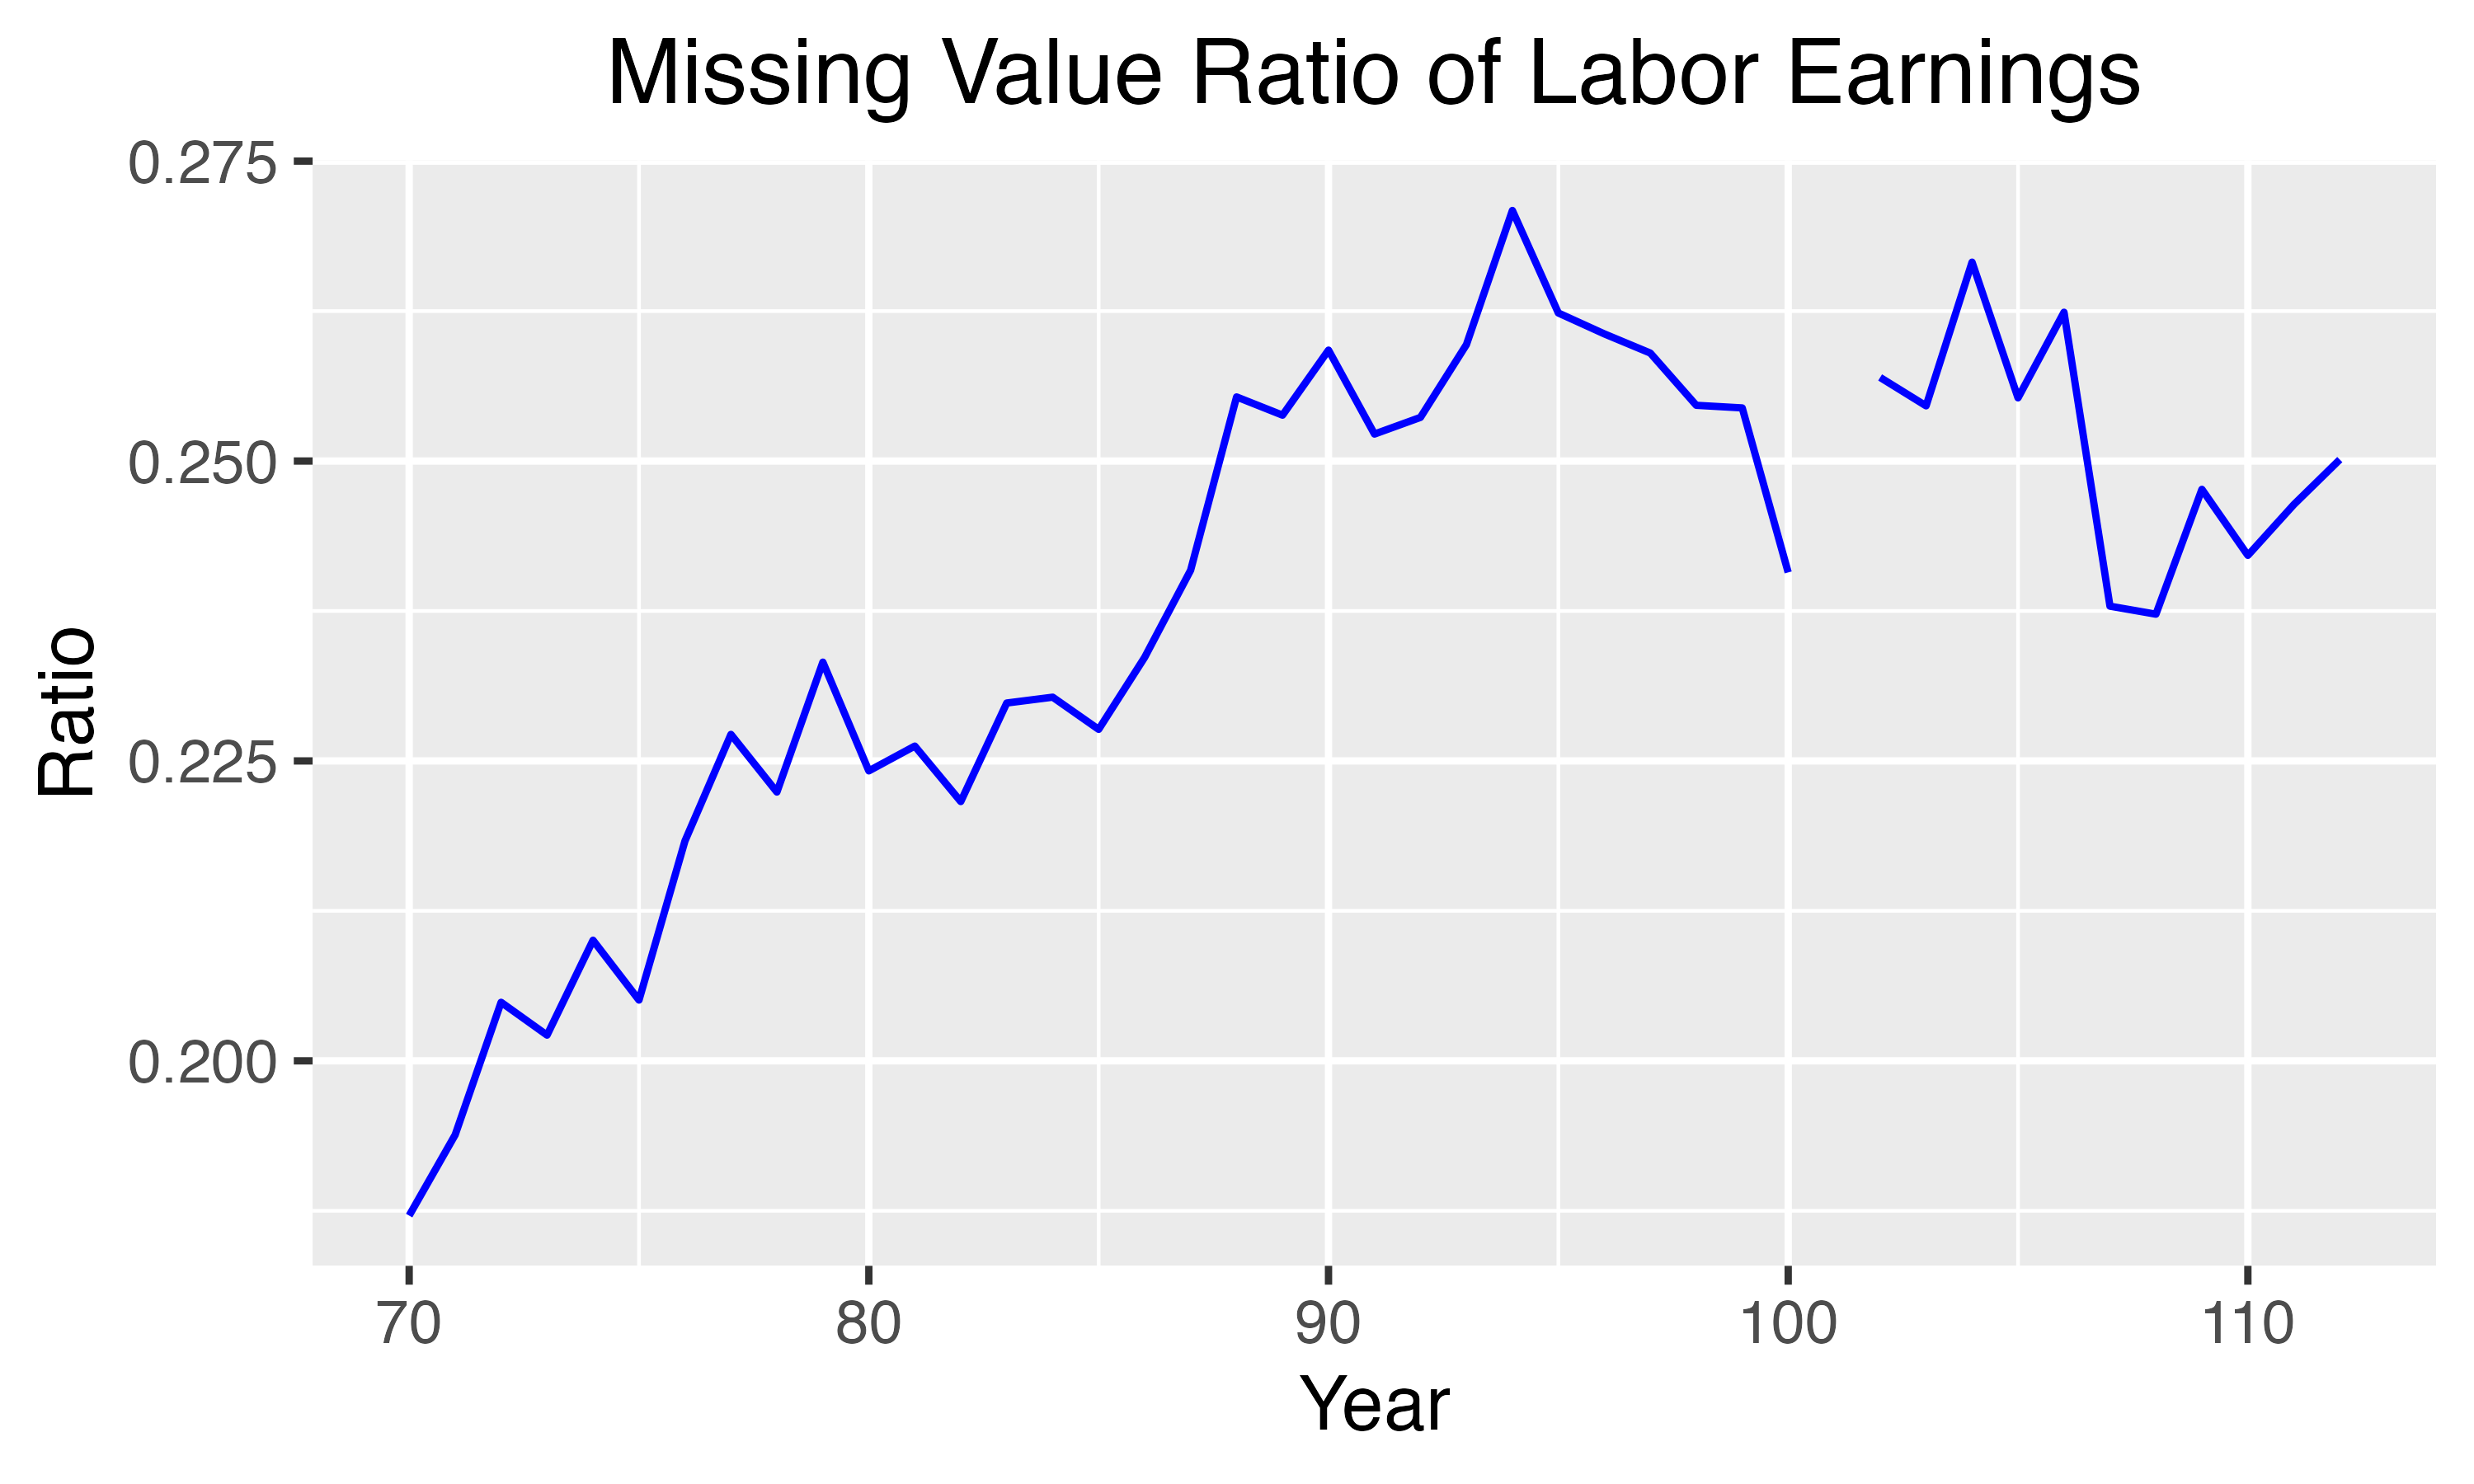
\includegraphics[width=\textwidth]{figures/missing/itm190.png}
    \end{subfigure}
    \begin{subfigure}[t]{0.475\textwidth}
        \centering
        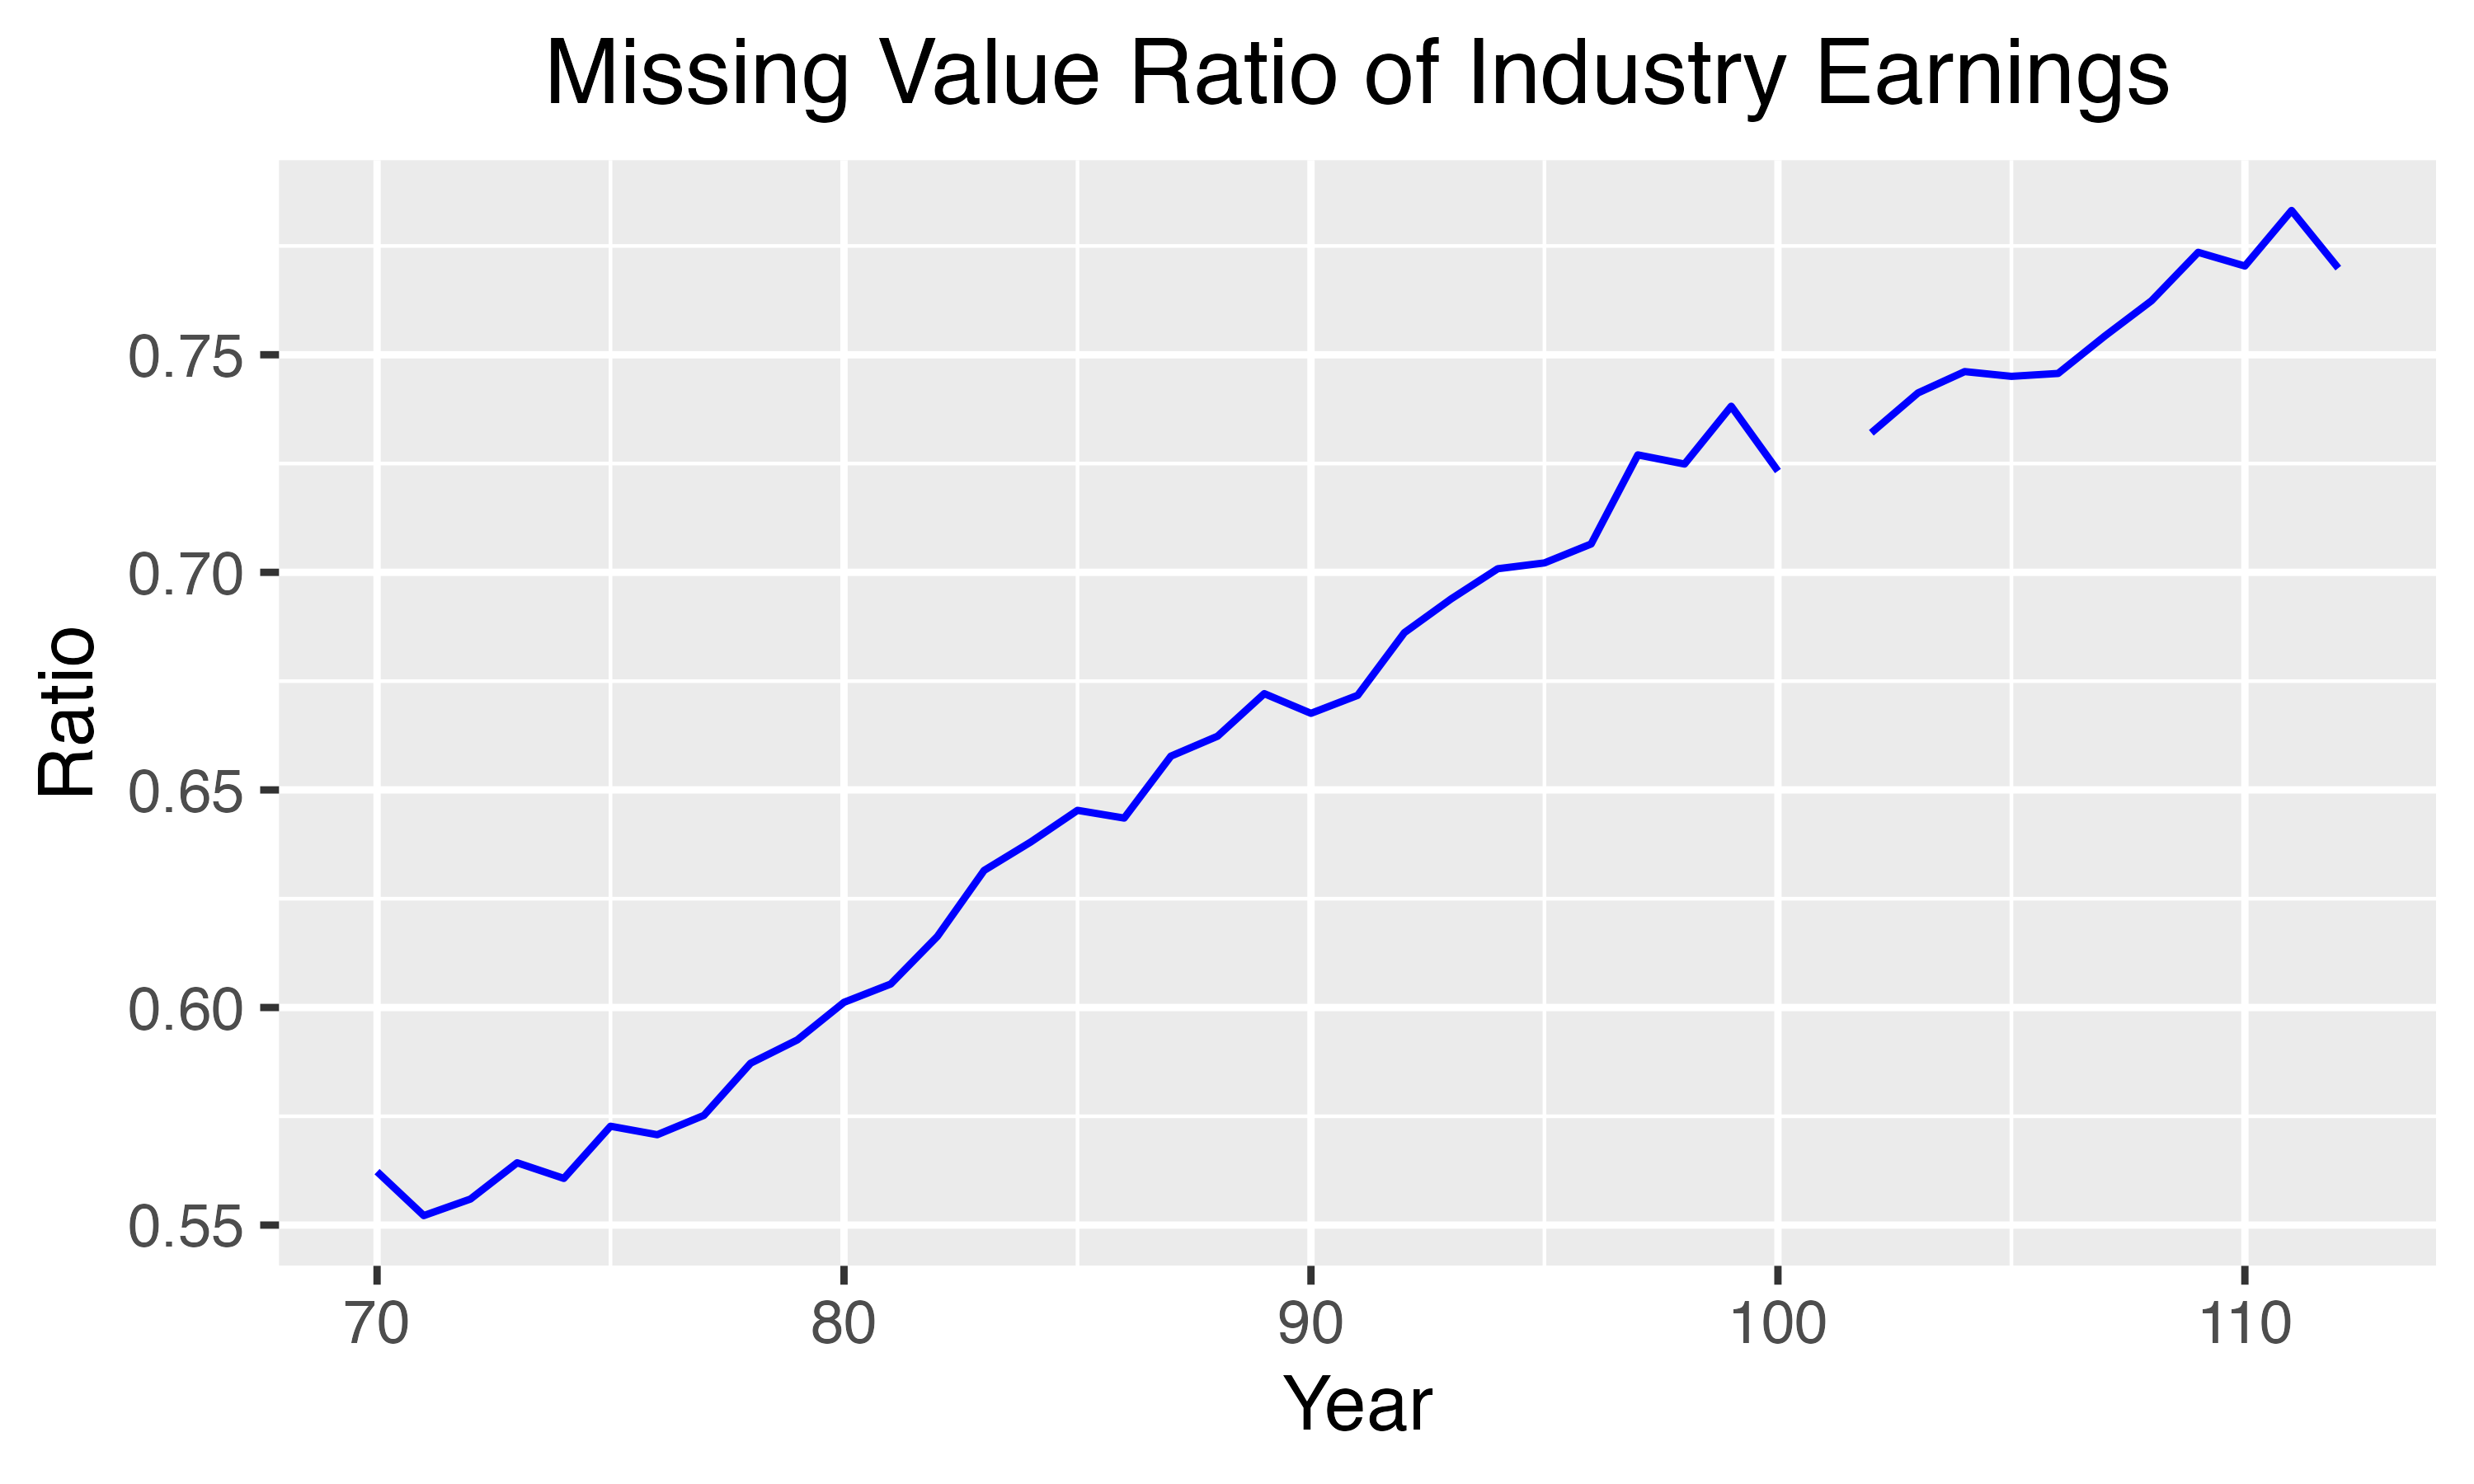
\includegraphics[width=\textwidth]{figures/missing/itm240.png}
    \end{subfigure}
    \caption{Missing Rate of Labor Earnings and Industry Earnings in SFIE}
    \label{fig:missing}
\end{figure}
In the SFIE, both zero and no response are treated as missing values, which can lead to an underestimation of income and consumption inequality if we treat all missing values as zero.
Therefore, the analysis in this paper will focus on households with positive earnings and consumption expenditures aligned with the design proposed by Heathcote, Perri, \& Violante (\citeyear{HEATHCOTE_2010}).
I treat the missing values as zero when doing addition and subtraction, such as calculating household earnings as the sum of labor and industry earnings.
Note that there is a missing value in 2012 of Figure \ref{fig:missing}, this is because the data file of SFIE for 2012 has all the demographic information, but the income and expenditure data are ALL missing values.
Therefore, I exclude the 2012 data from the analysis.

\subsection{CPI adjustment}

The SFIE provides nominal values for income and expenditures, which need to be adjusted for inflation to obtain real values. 
The price deflator used in this paper is the Consumer Price Index (\citelink{DGBAS_CPI}{CPI}) provided by the \citeauthor{DGBAS_CPI}.
Figure \ref{fig:CPI} shows the CPI in Taiwan from 1981 to 2023 normalized to 100 in 2021.
\begin{figure}
    \centering
    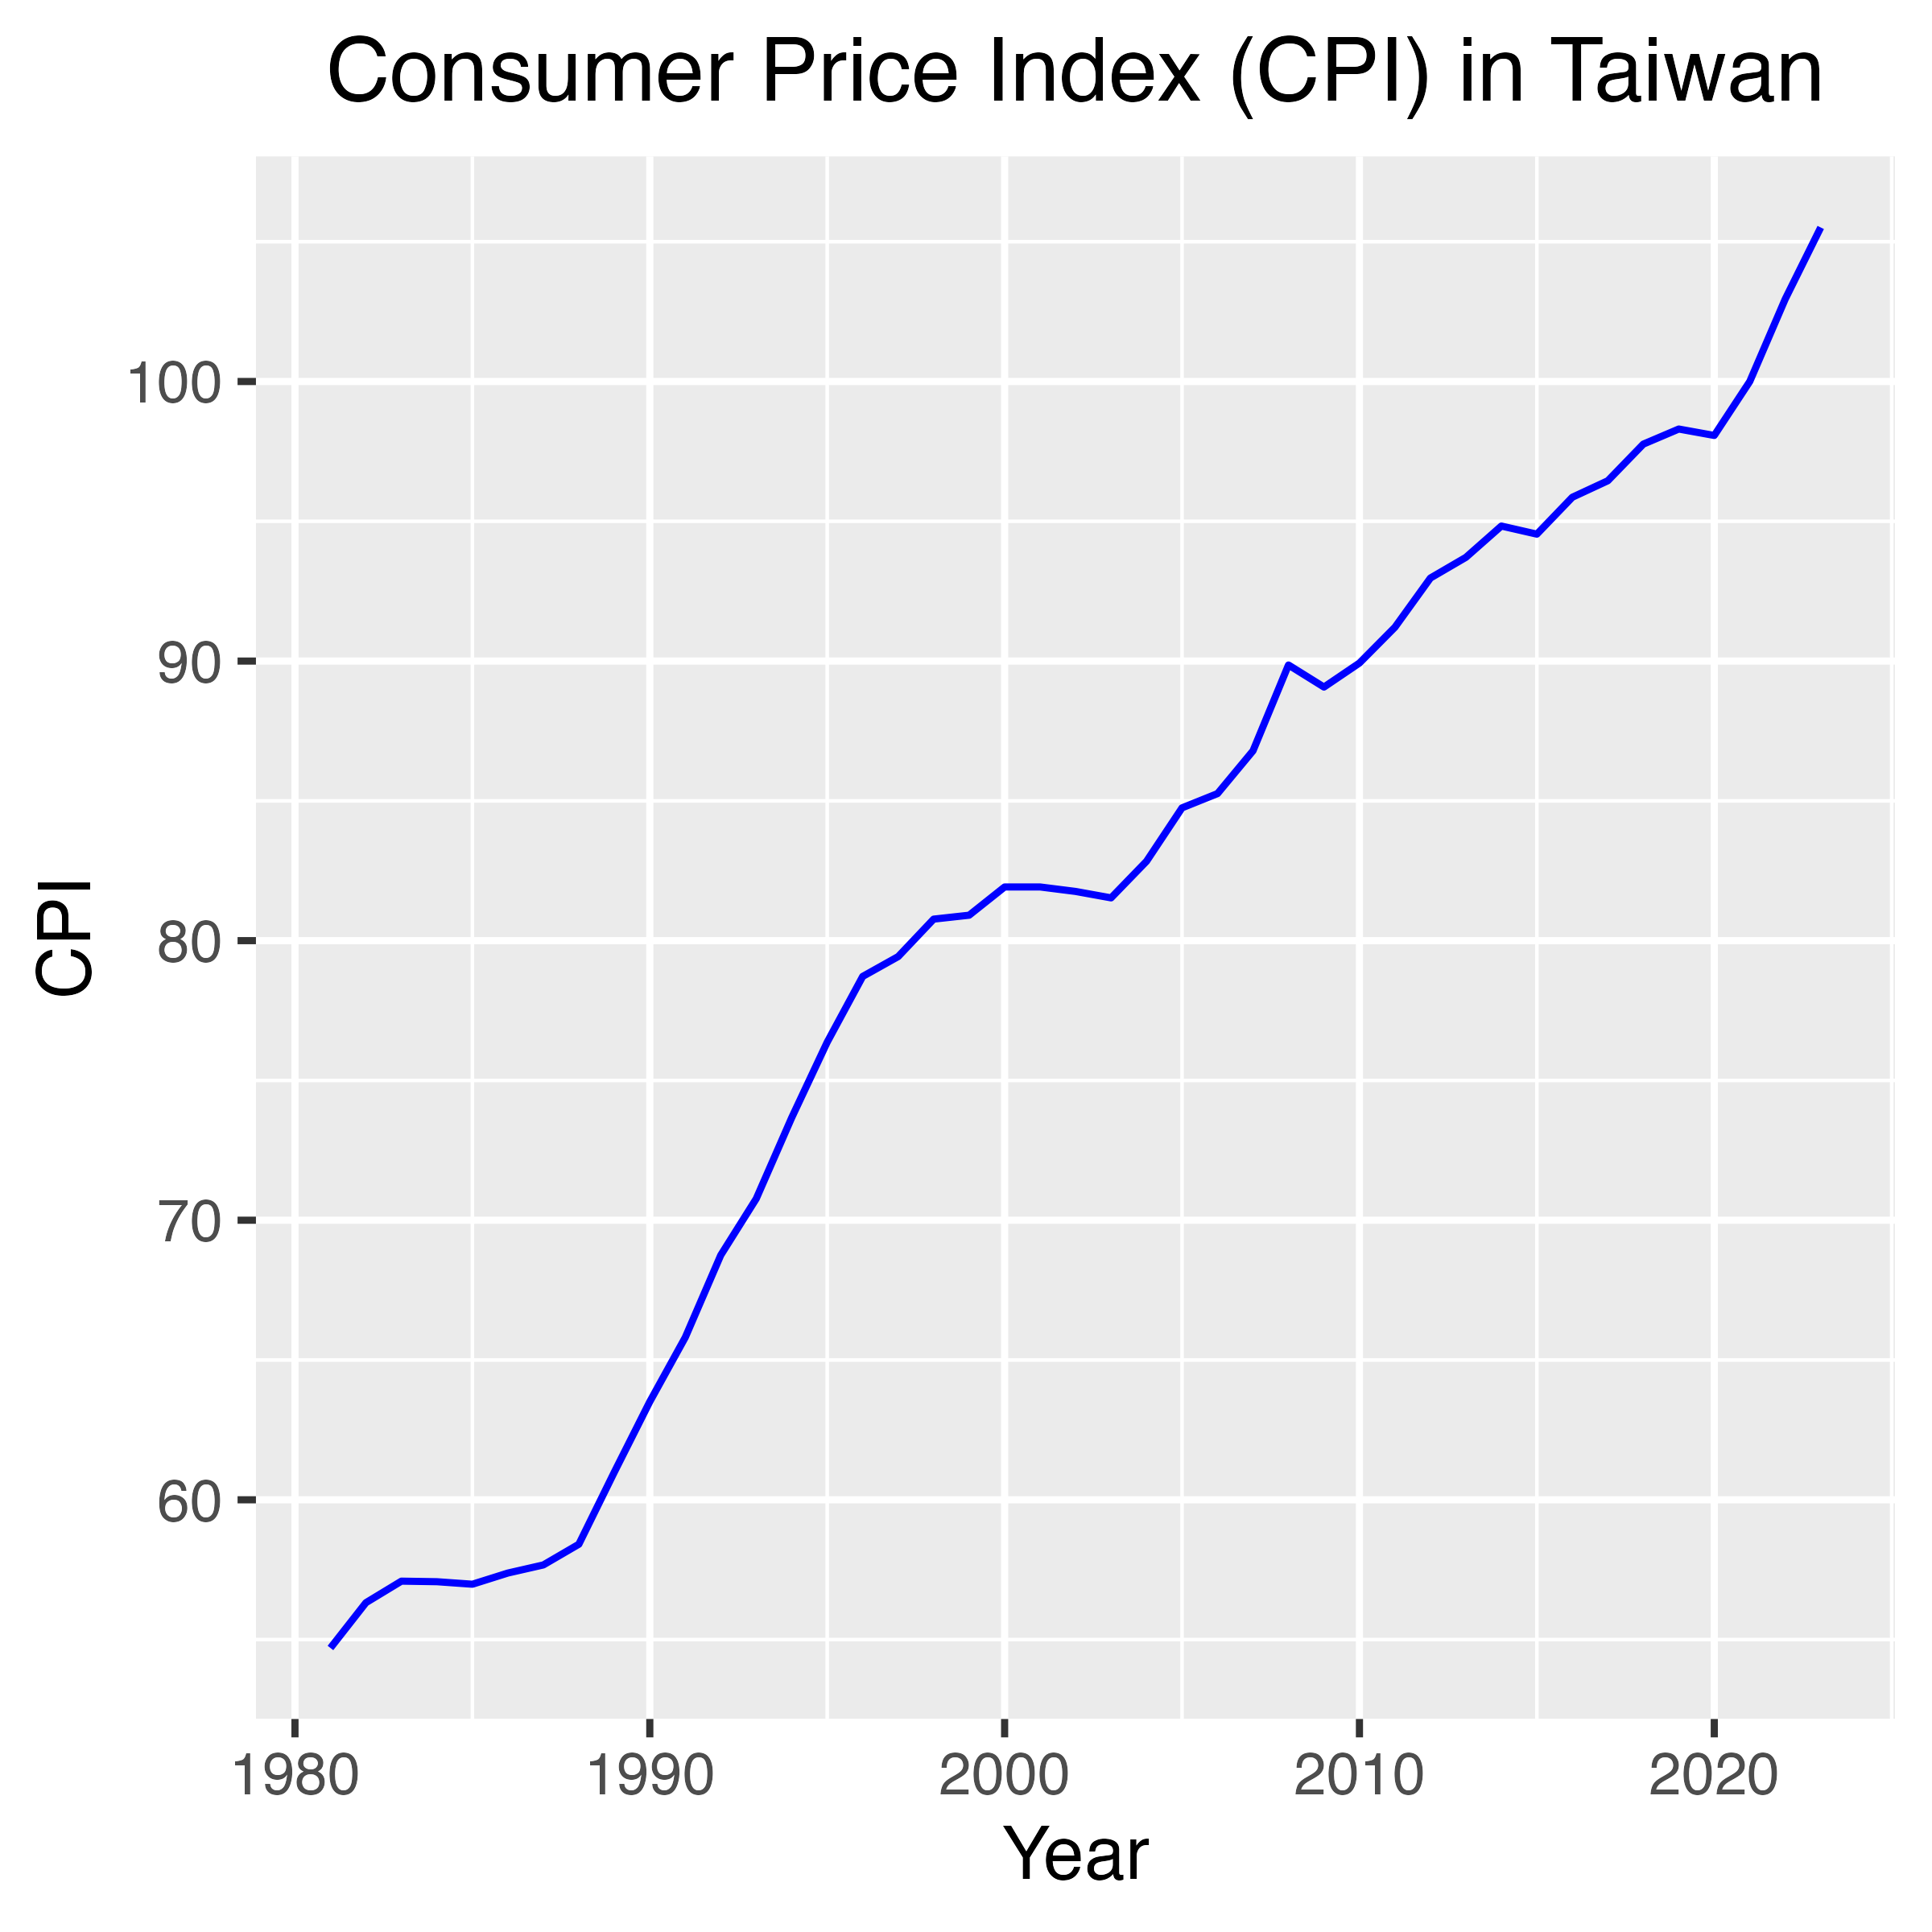
\includegraphics[width=0.475\textwidth]{figures/cpi.png}
    \caption{Consumer Price Index (CPI) in Taiwan, 1981 - 2023}
    \label{fig:CPI}
\end{figure}

\subsection{Equivalize Household Income and Consumption}

To compare households of different sizes and compositions, I use the OECD equivalence scale to adjust household income and consumption to per-adult-equivalent levels. The OECD scale assigns a weight of 1 to the first adult, 0.7 to each additional adult, and 0.5 to each child. For the definition of child, I define a child as age 17 or younger, the original OECD definition is age 13 or younger.

\section{Household-level Inequality}
\label{sec:household_inequality}

Here, I present the household-level inequality measures, including earnings and consumption inequality, and their cyclical dynamics. This paper skips individual-level inequality, as it is more suitable to estimate using tax records. Individual-level consumption is not available in the SFIE, as it only recordes household-level non-durable consumption.
Estimating consumption inequality using household-level data is also more suitable, as households can share consumption goods and services, such as housing and food, which are not easily separable at the individual level.
In this section, I will follow the structure of Heathcote, Perri, \& Violante (\citeyear{HEATHCOTE_2010}) to construct a complete picture of household-level inequality from basic earnings to disposable income and consumption. 


\subsection{Inequality in Earnings}

\begin{figure}
    \centering
    \begin{subfigure}[t]{0.475\textwidth}
        \centering
        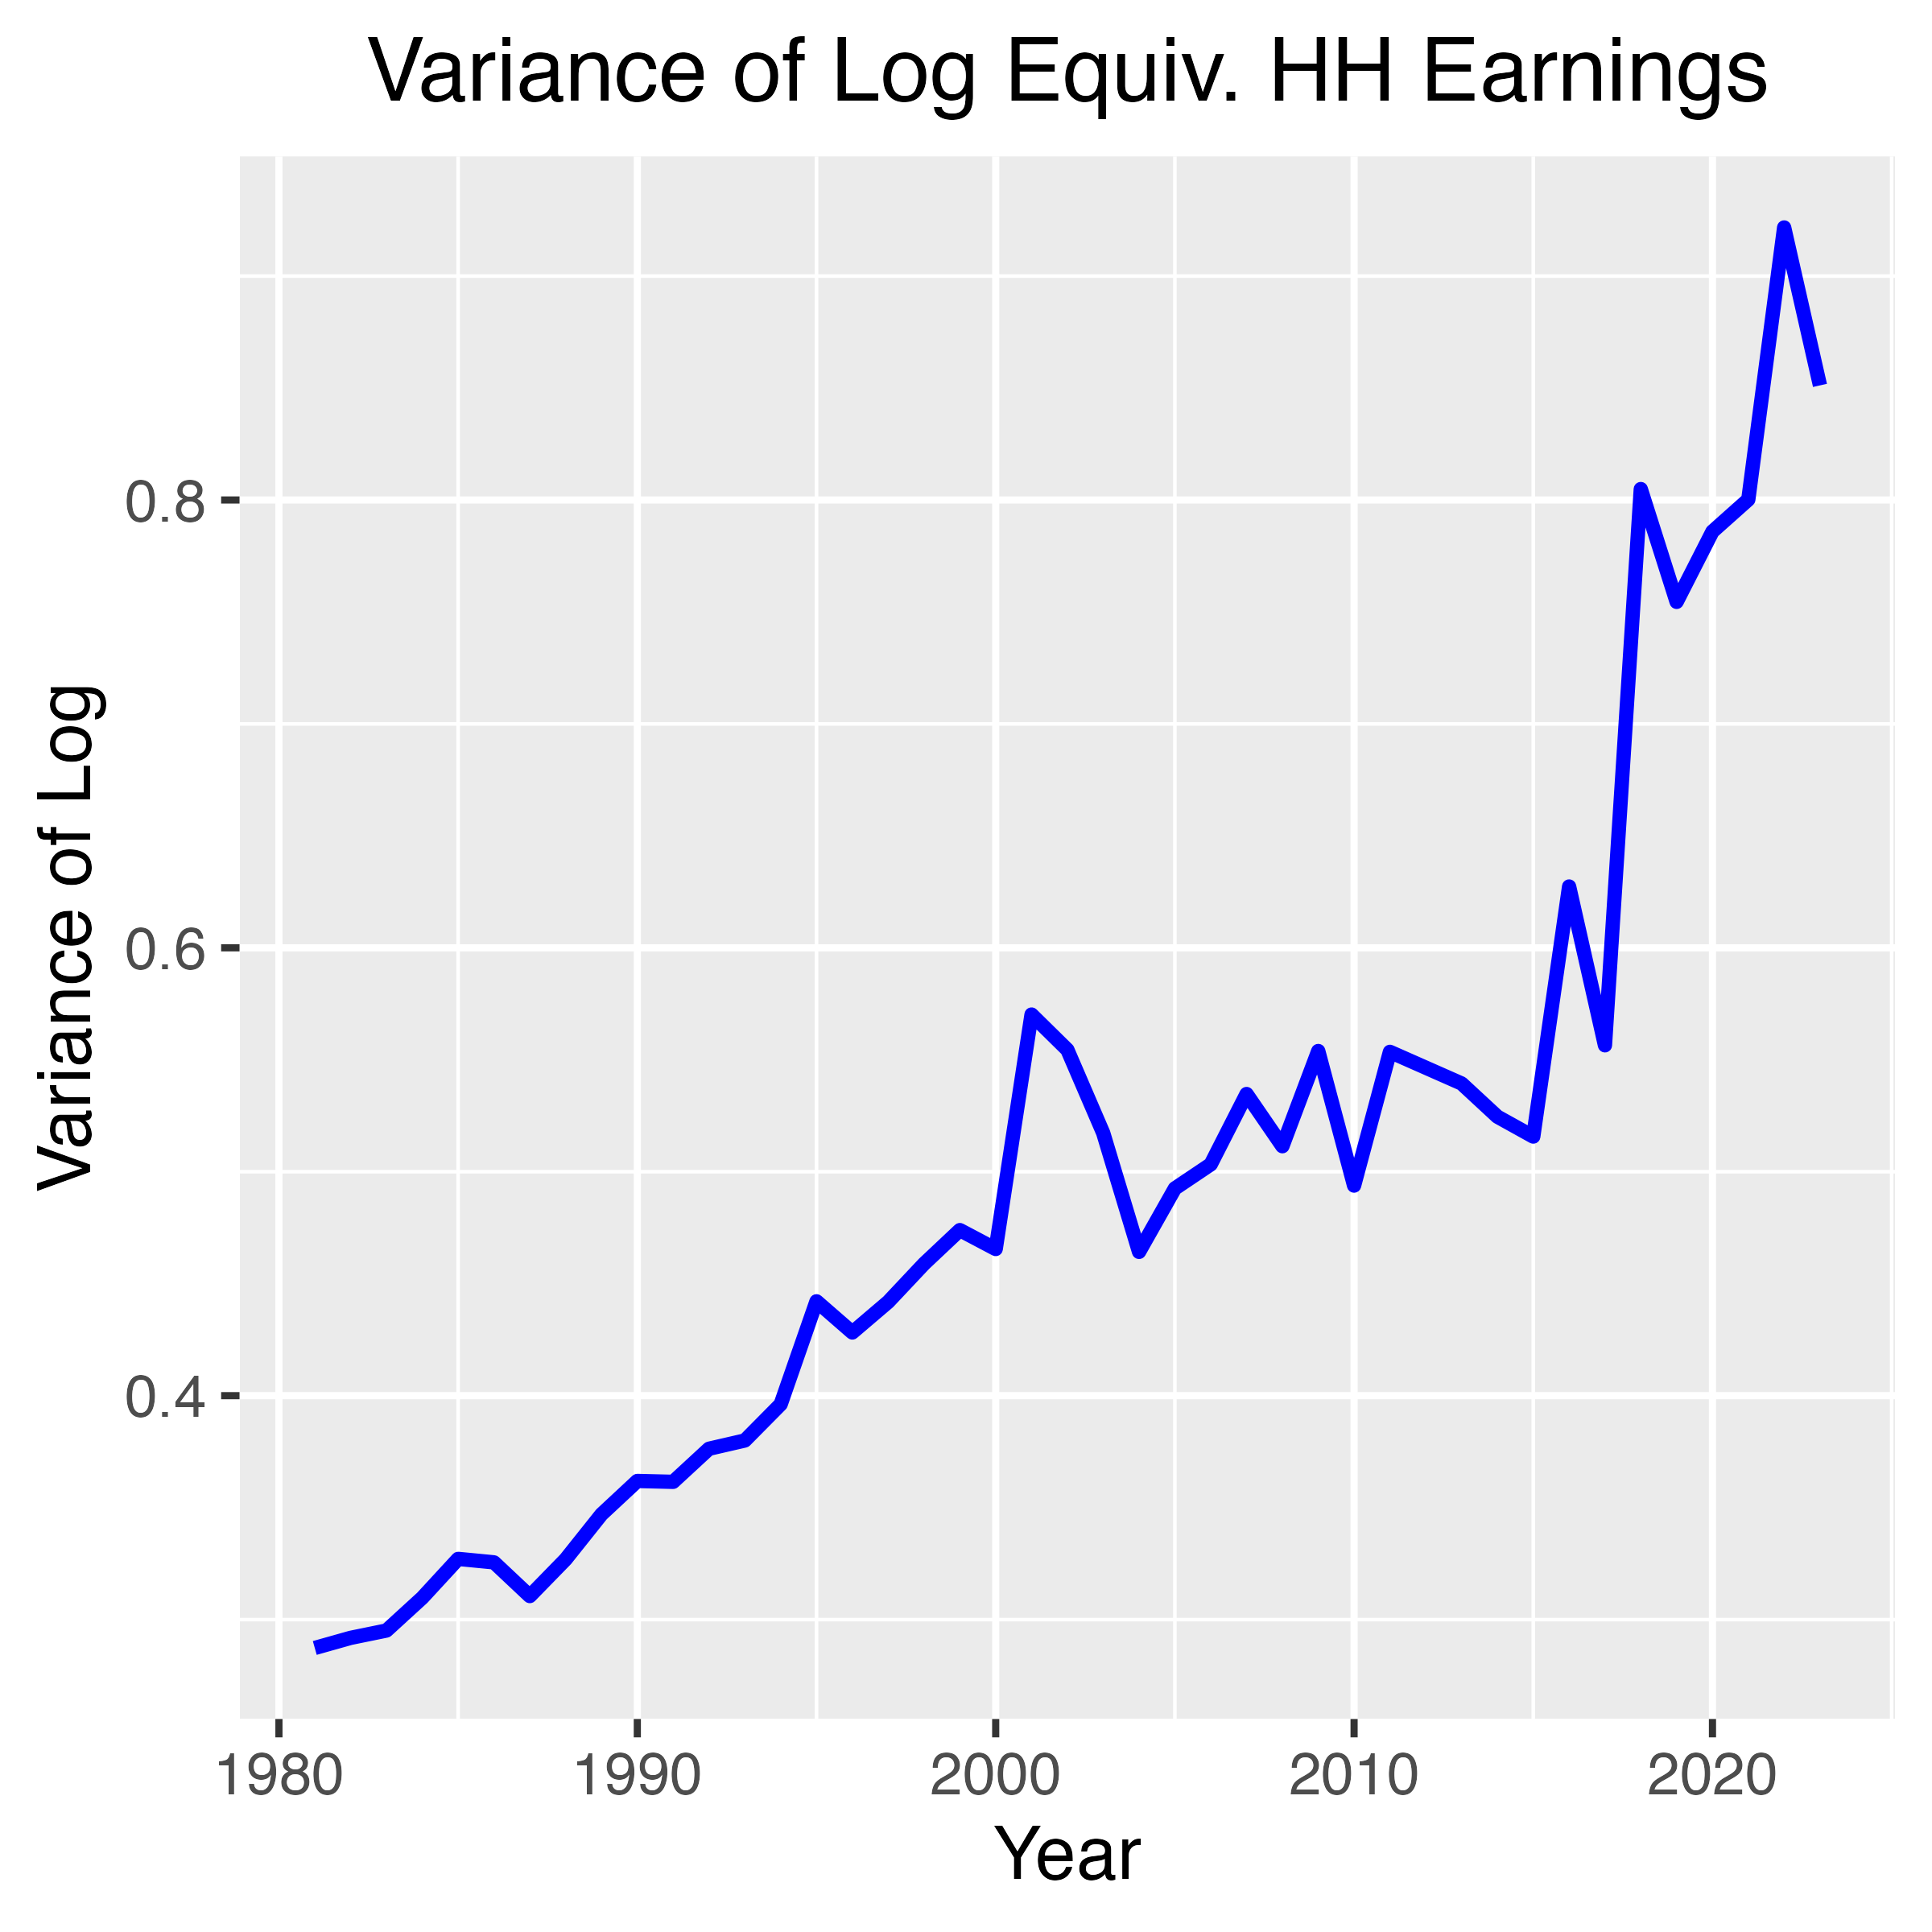
\includegraphics[width=\textwidth]{figures/Fig_1/Fig_1a_Var_Earnings.png}
    \end{subfigure}
    \begin{subfigure}[t]{0.475\textwidth}
        \centering
        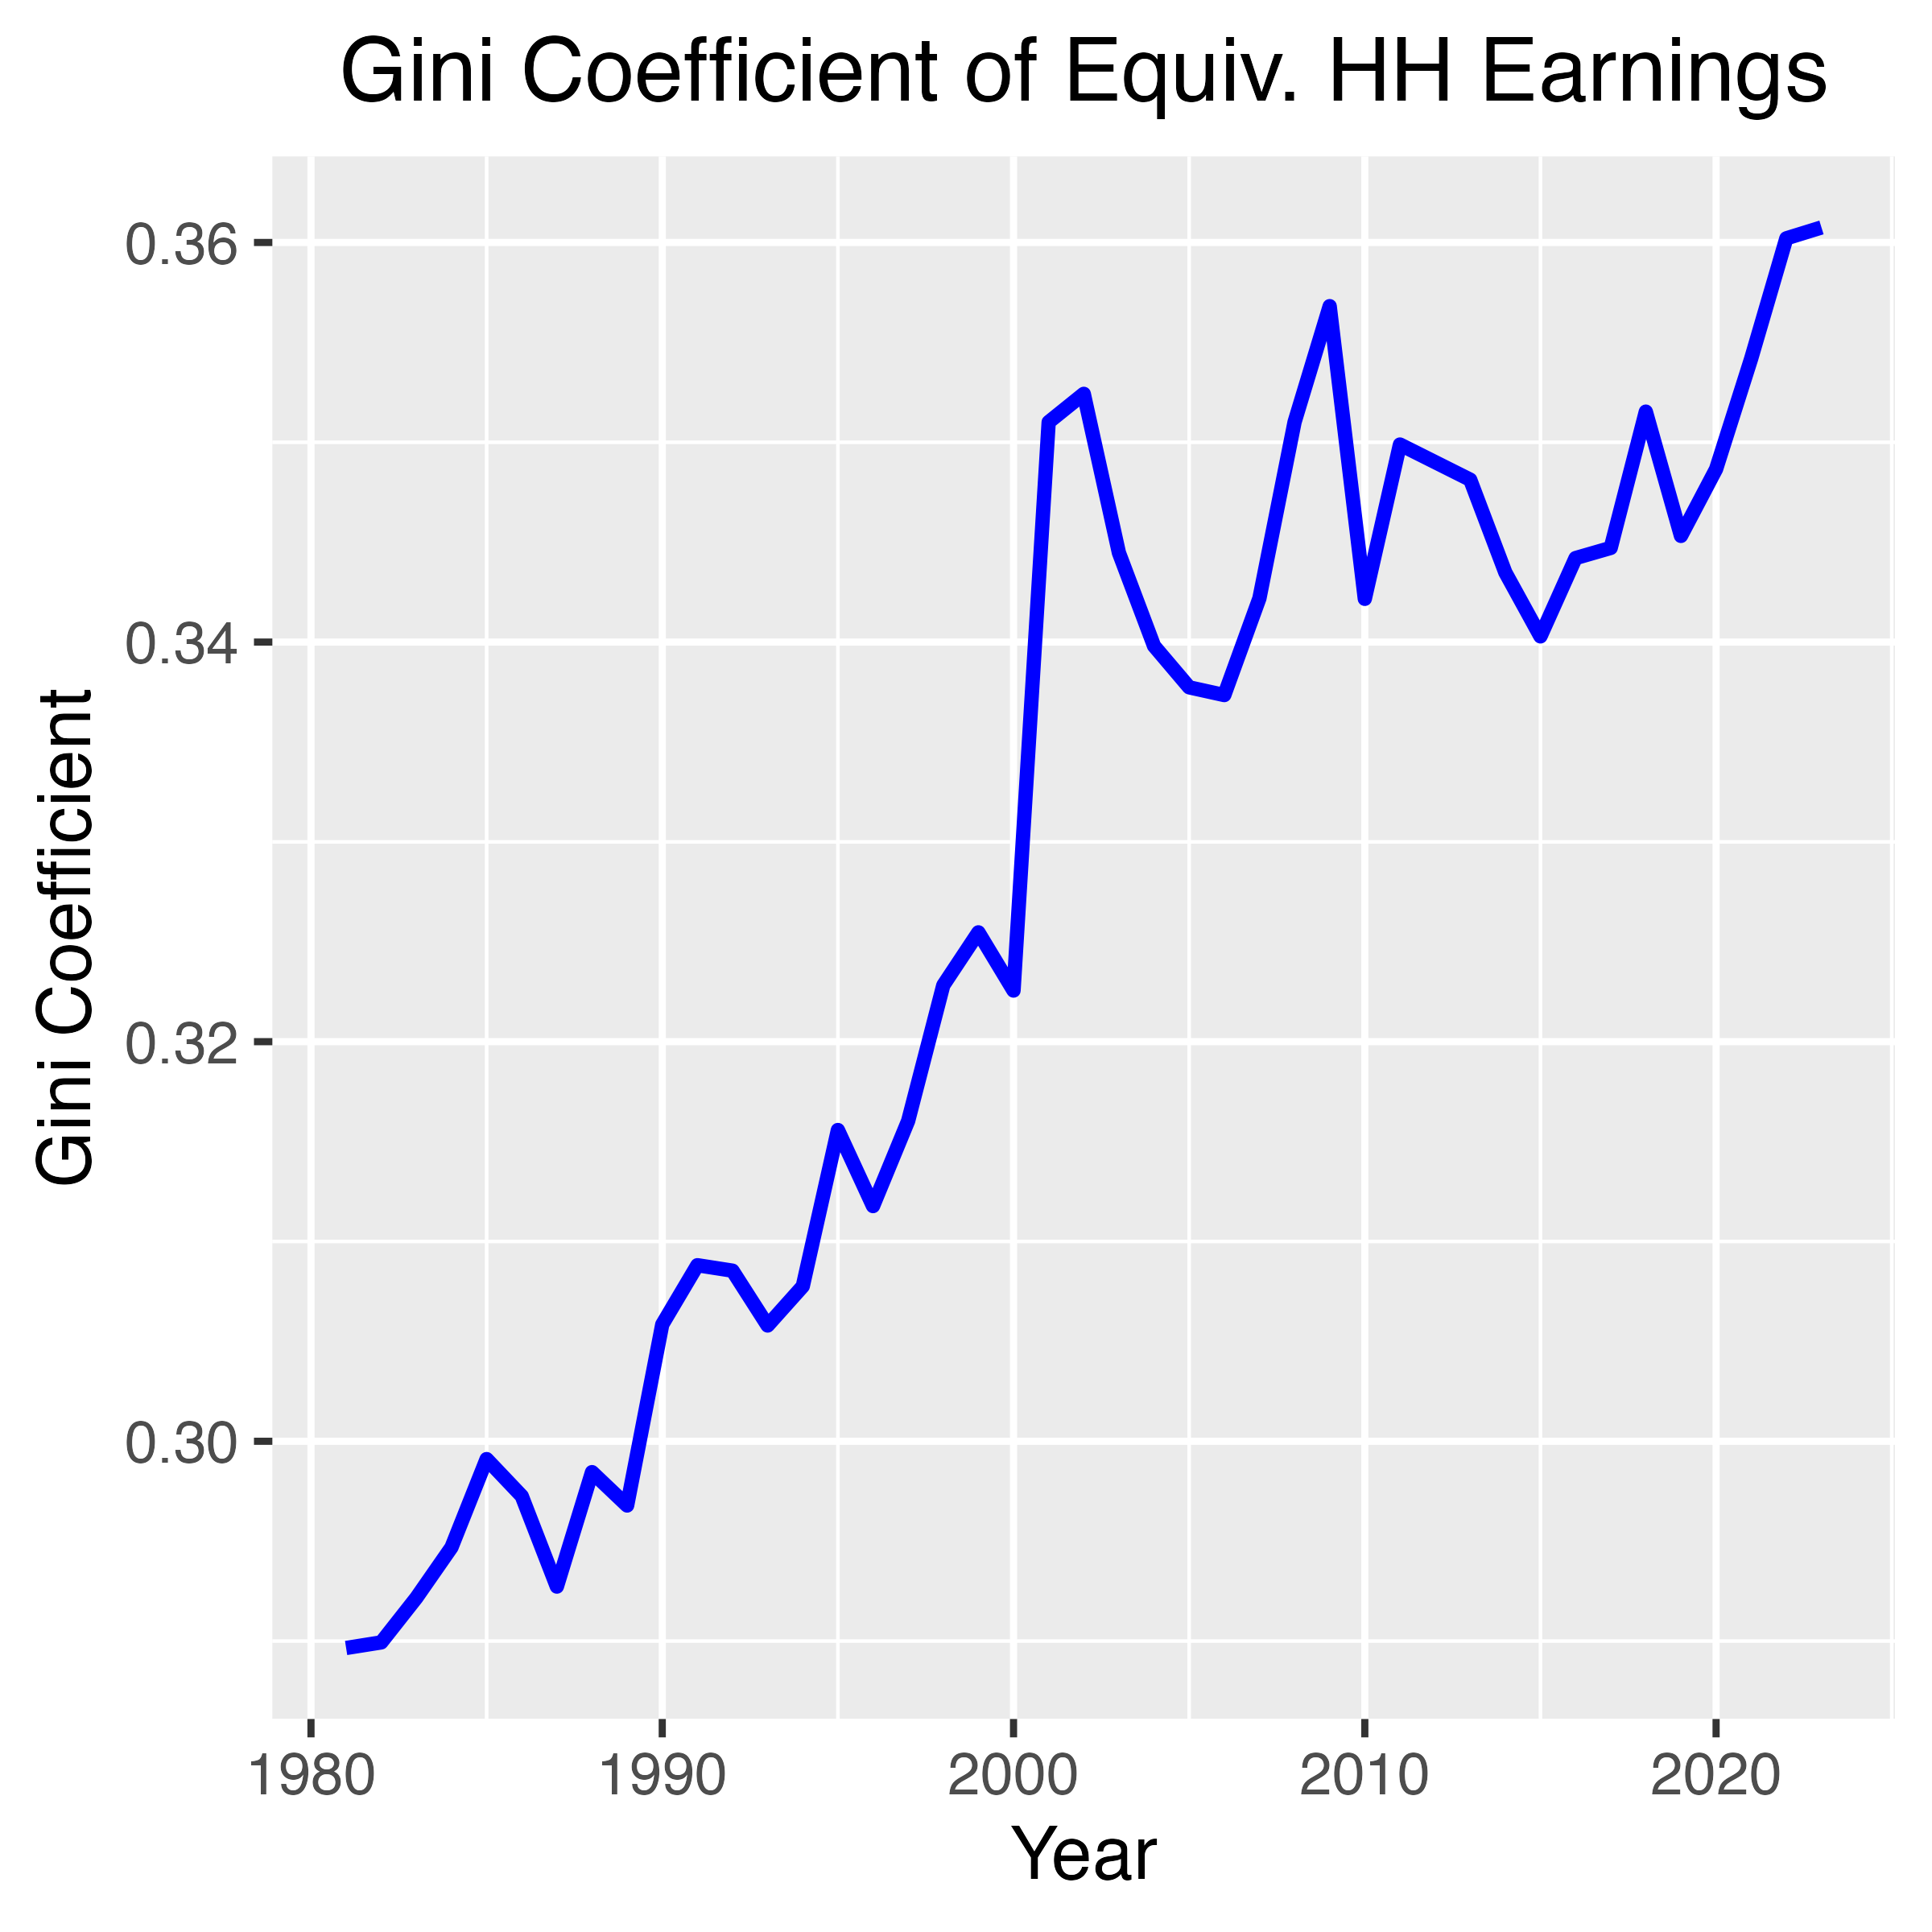
\includegraphics[width=\textwidth]{figures/Fig_1/Fig_1b_Gini_Earnings.png}
    \end{subfigure}
    \begin{subfigure}[t]{0.475\textwidth}
        \centering
        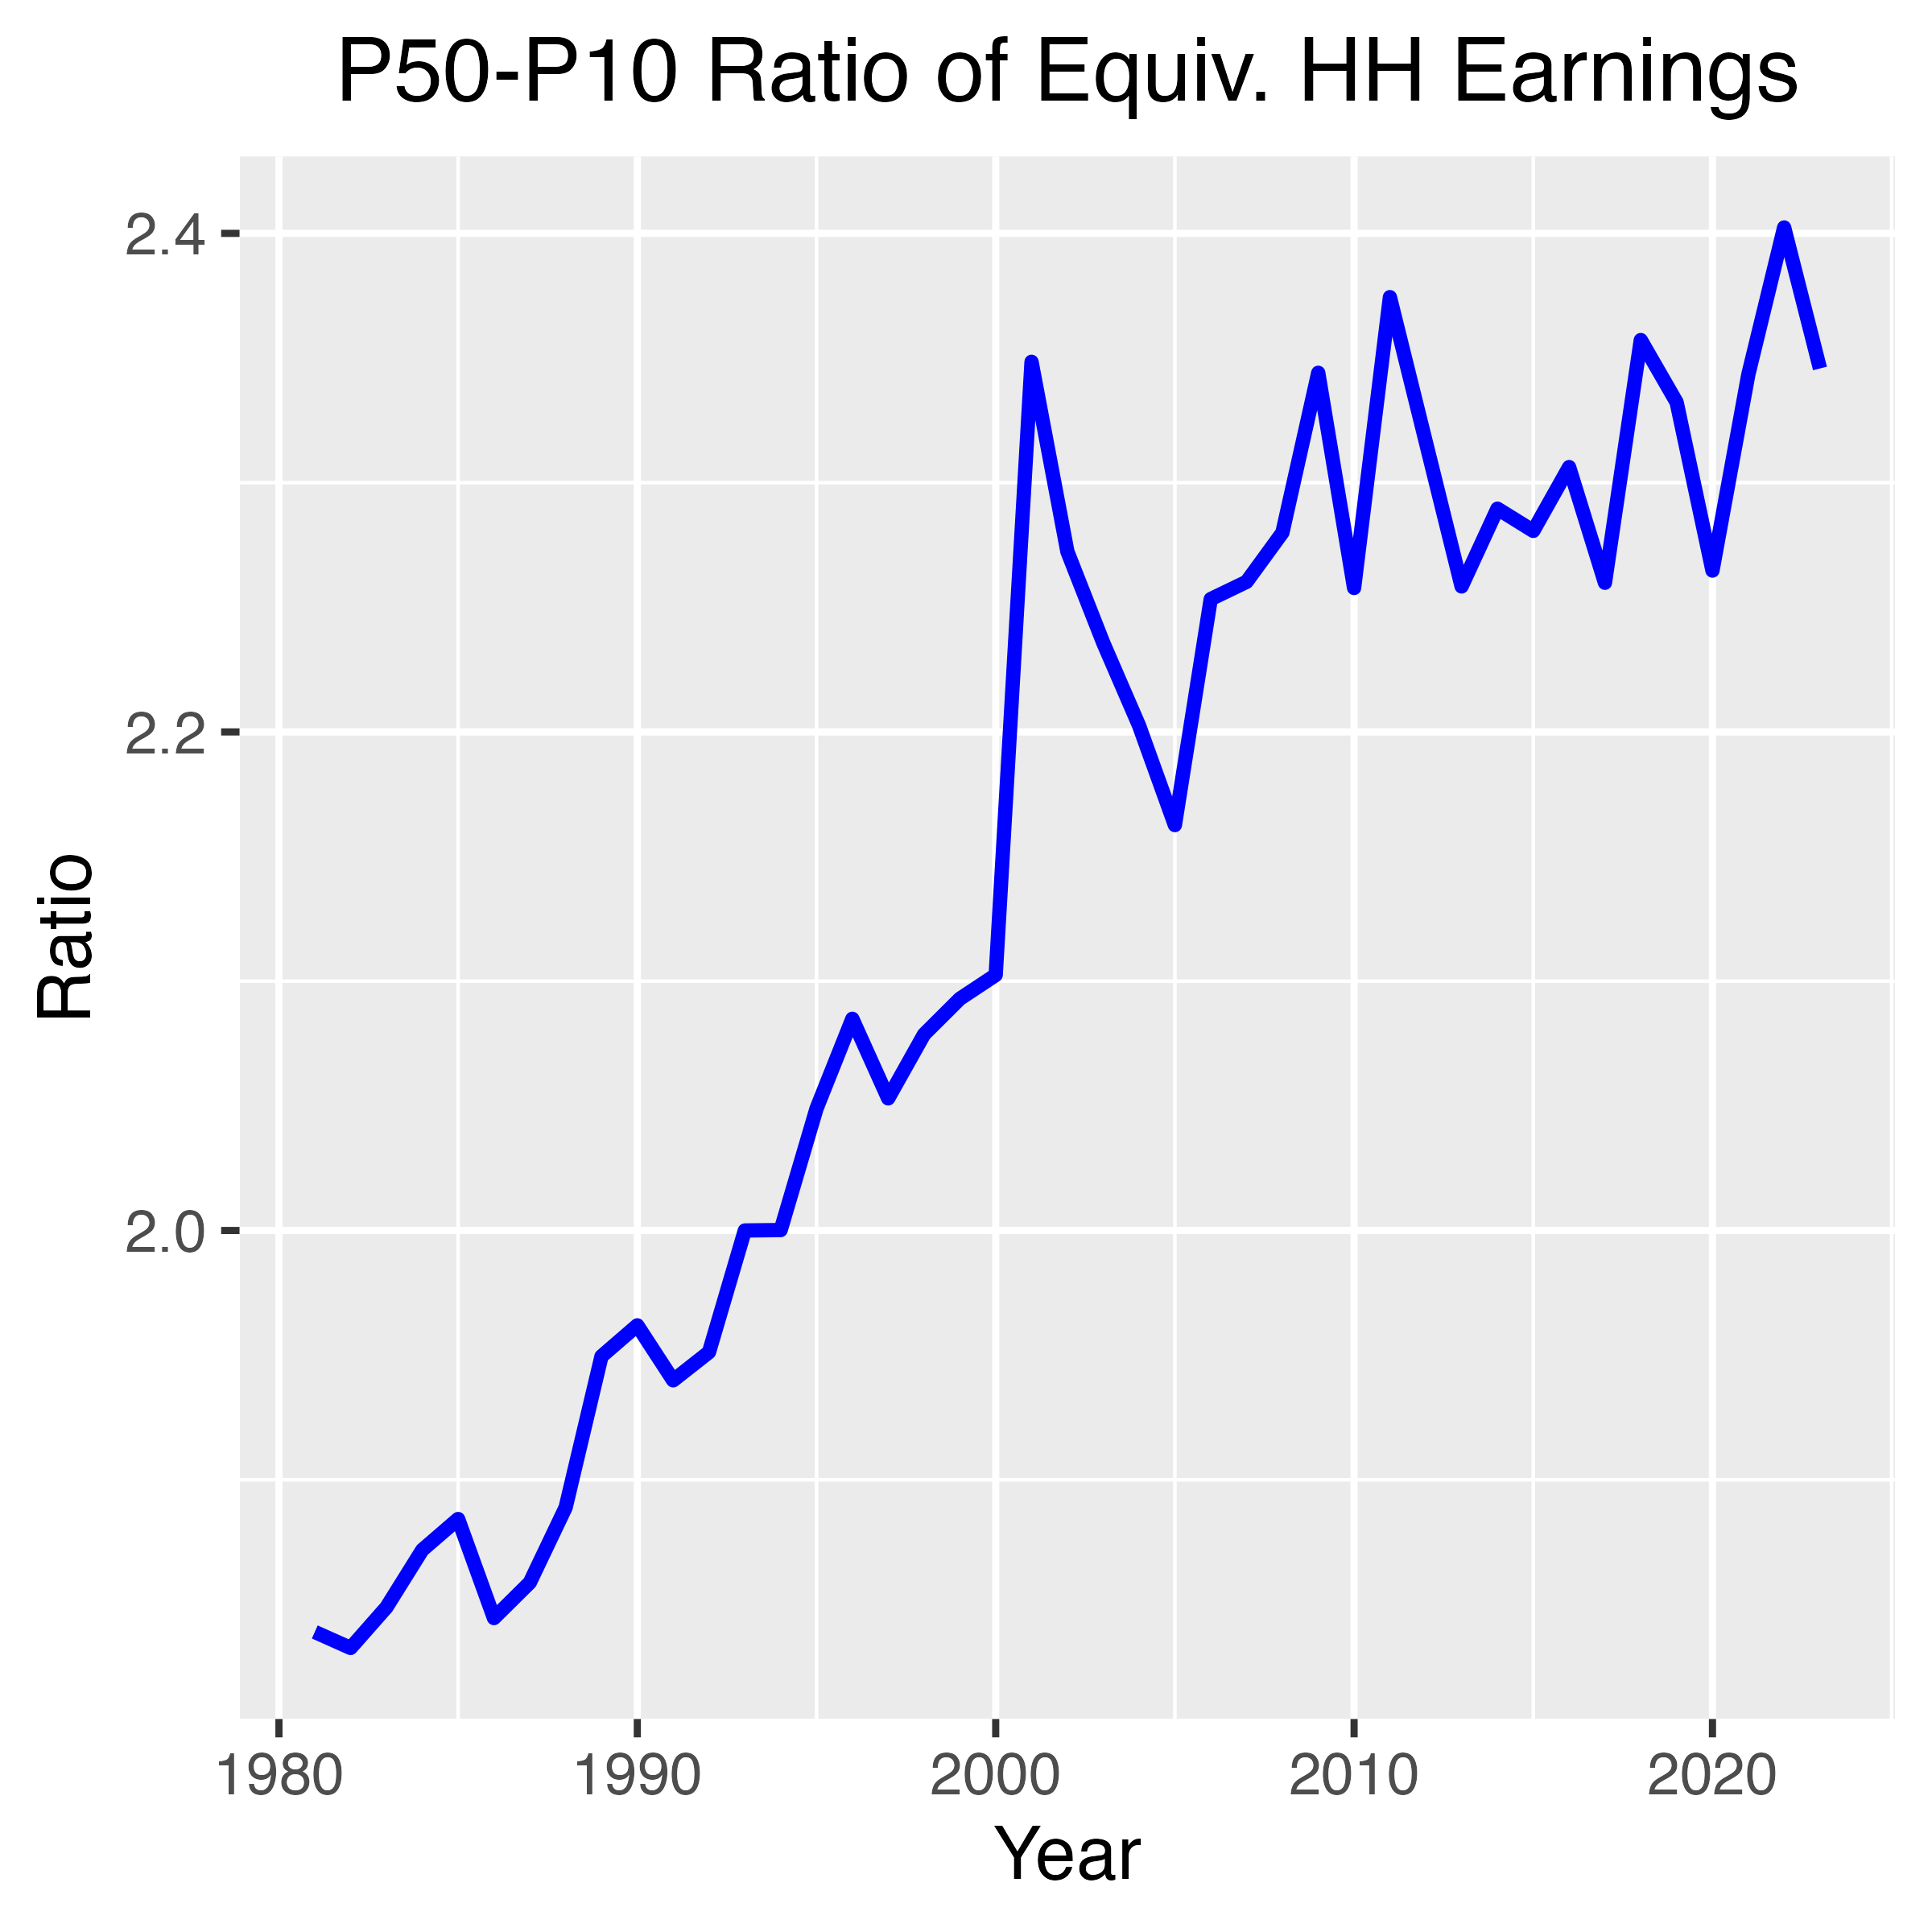
\includegraphics[width=\textwidth]{figures/Fig_1/Fig_1c_P50_P10_Earnings.png}
    \end{subfigure}
    \begin{subfigure}[t]{0.475\textwidth}
        \centering
        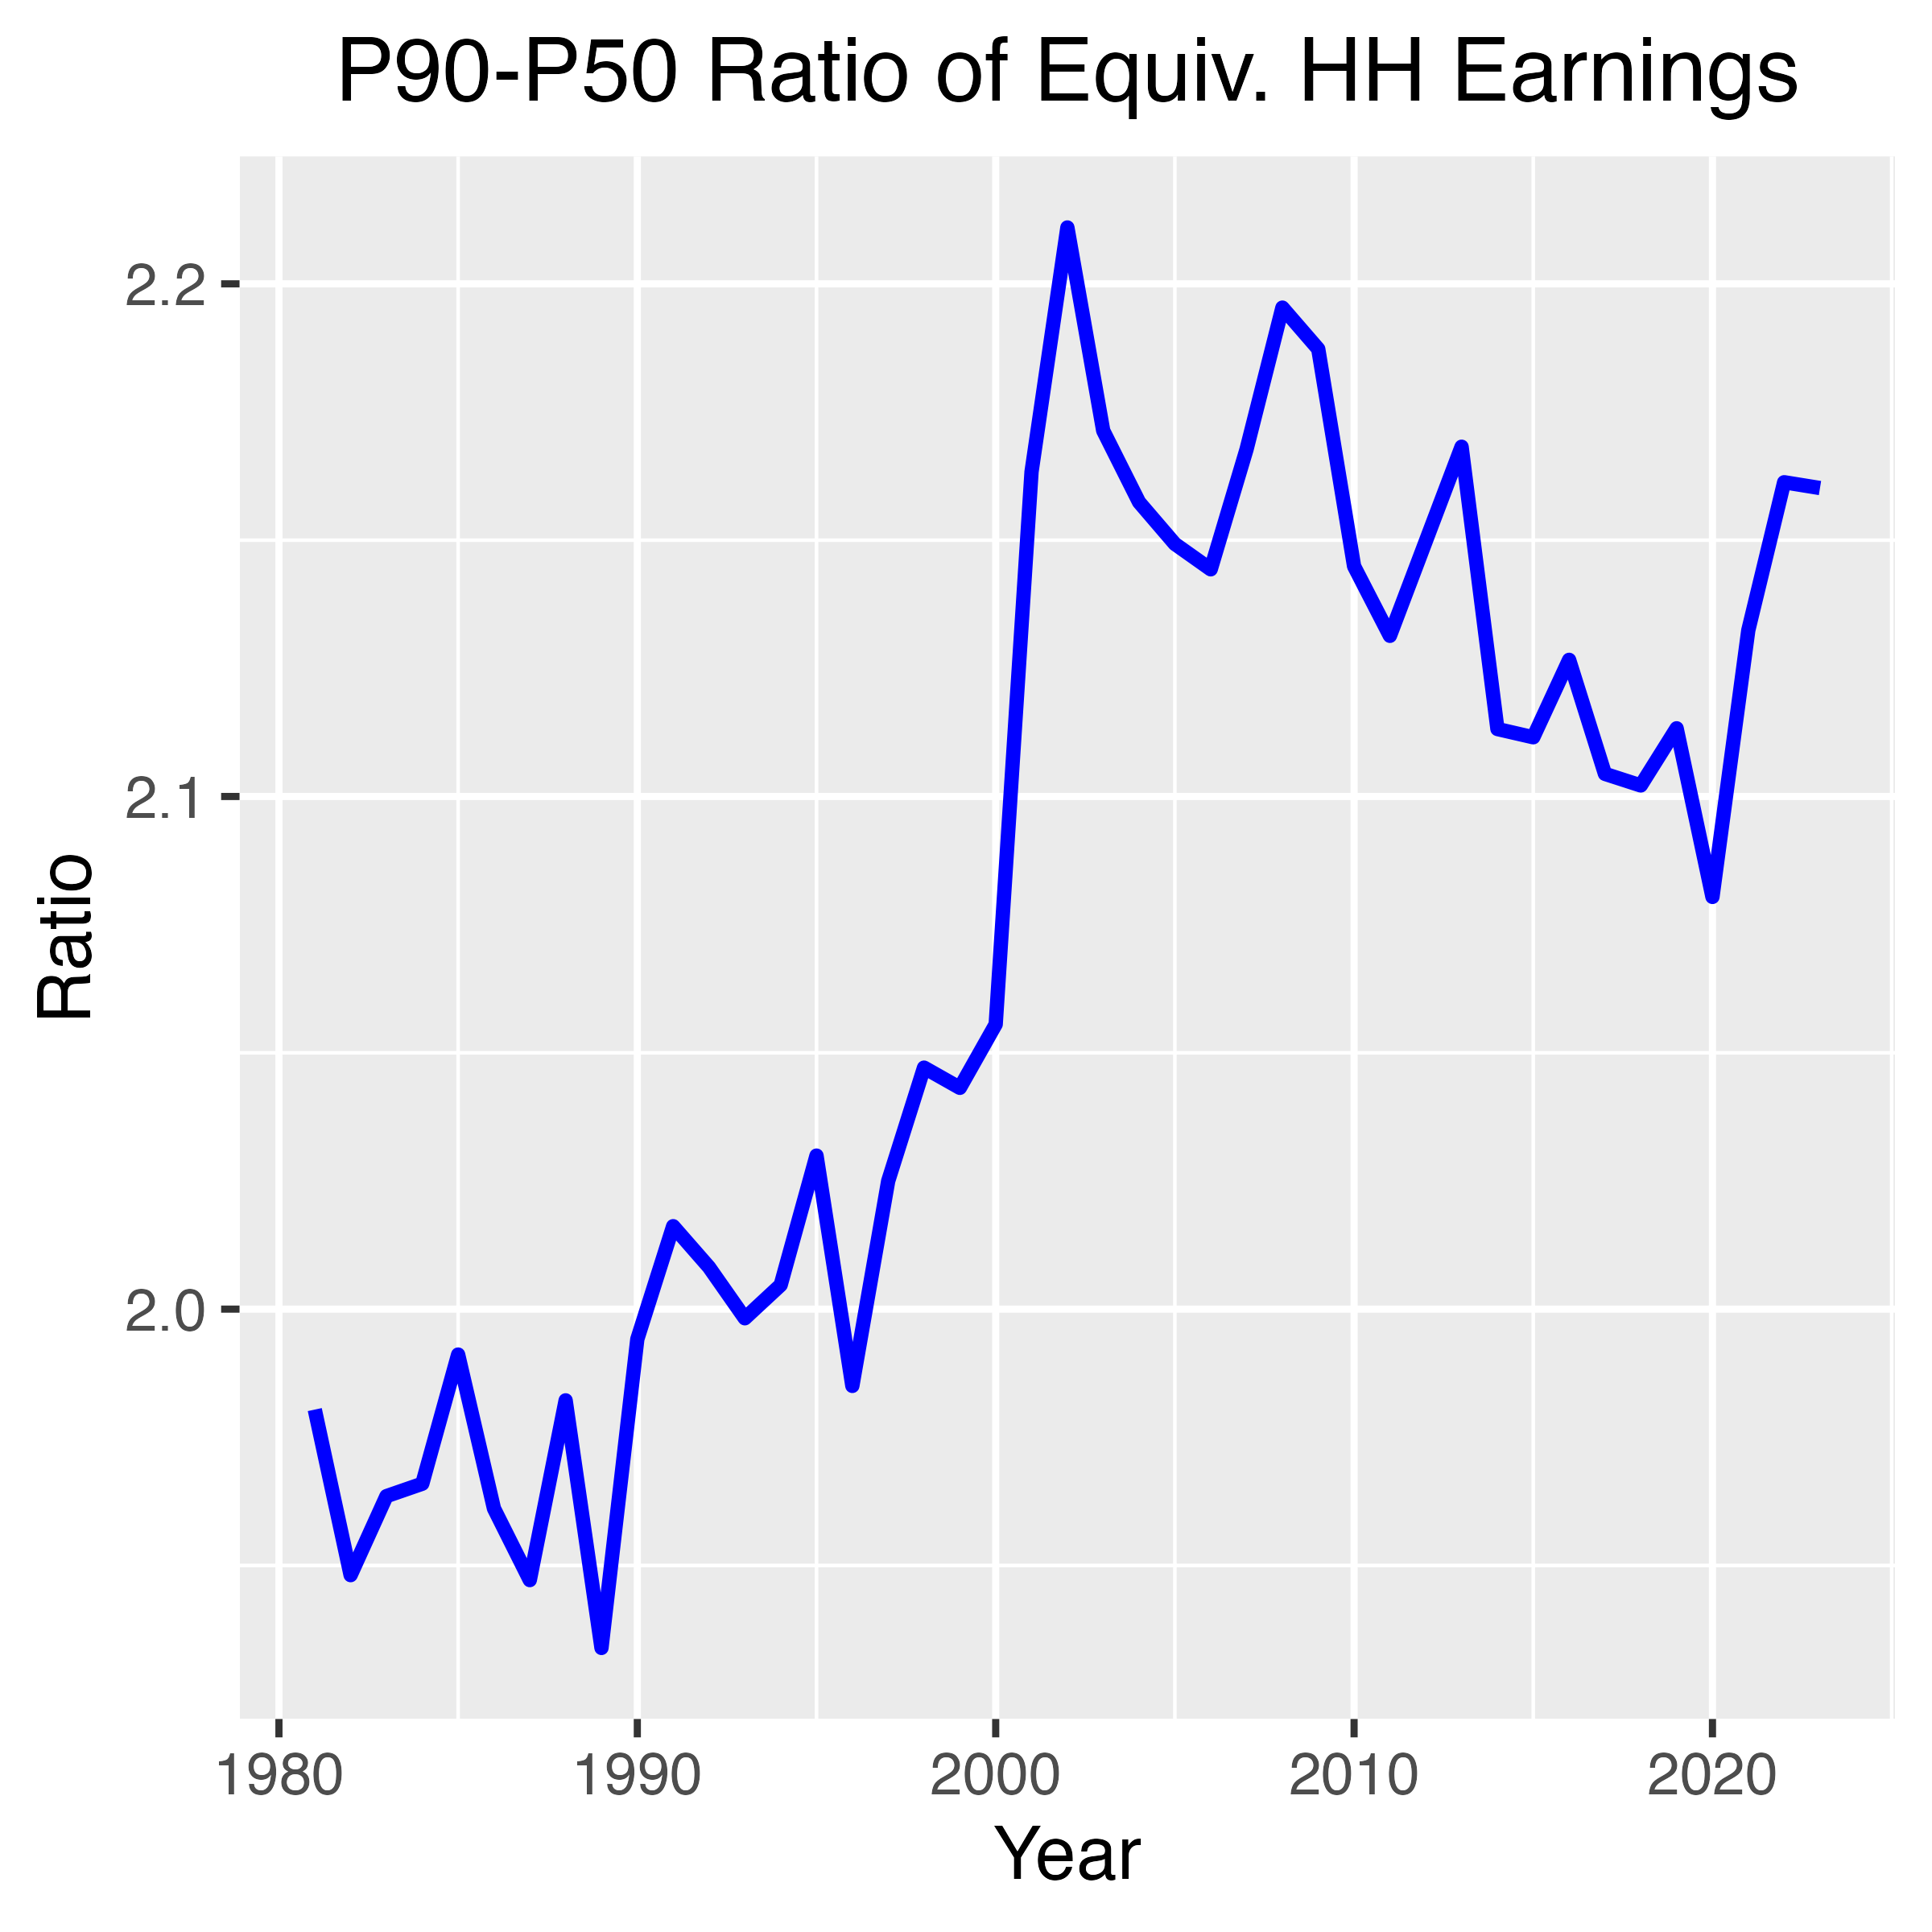
\includegraphics[width=\textwidth]{figures/Fig_1/Fig_1d_P90_P50_Earnings.png}
    \end{subfigure}
    \caption{Various Measures of Household Earnings Inequality}
    \label{fig:earnings_inequality}
\end{figure}

\begin{figure}
    \centering
    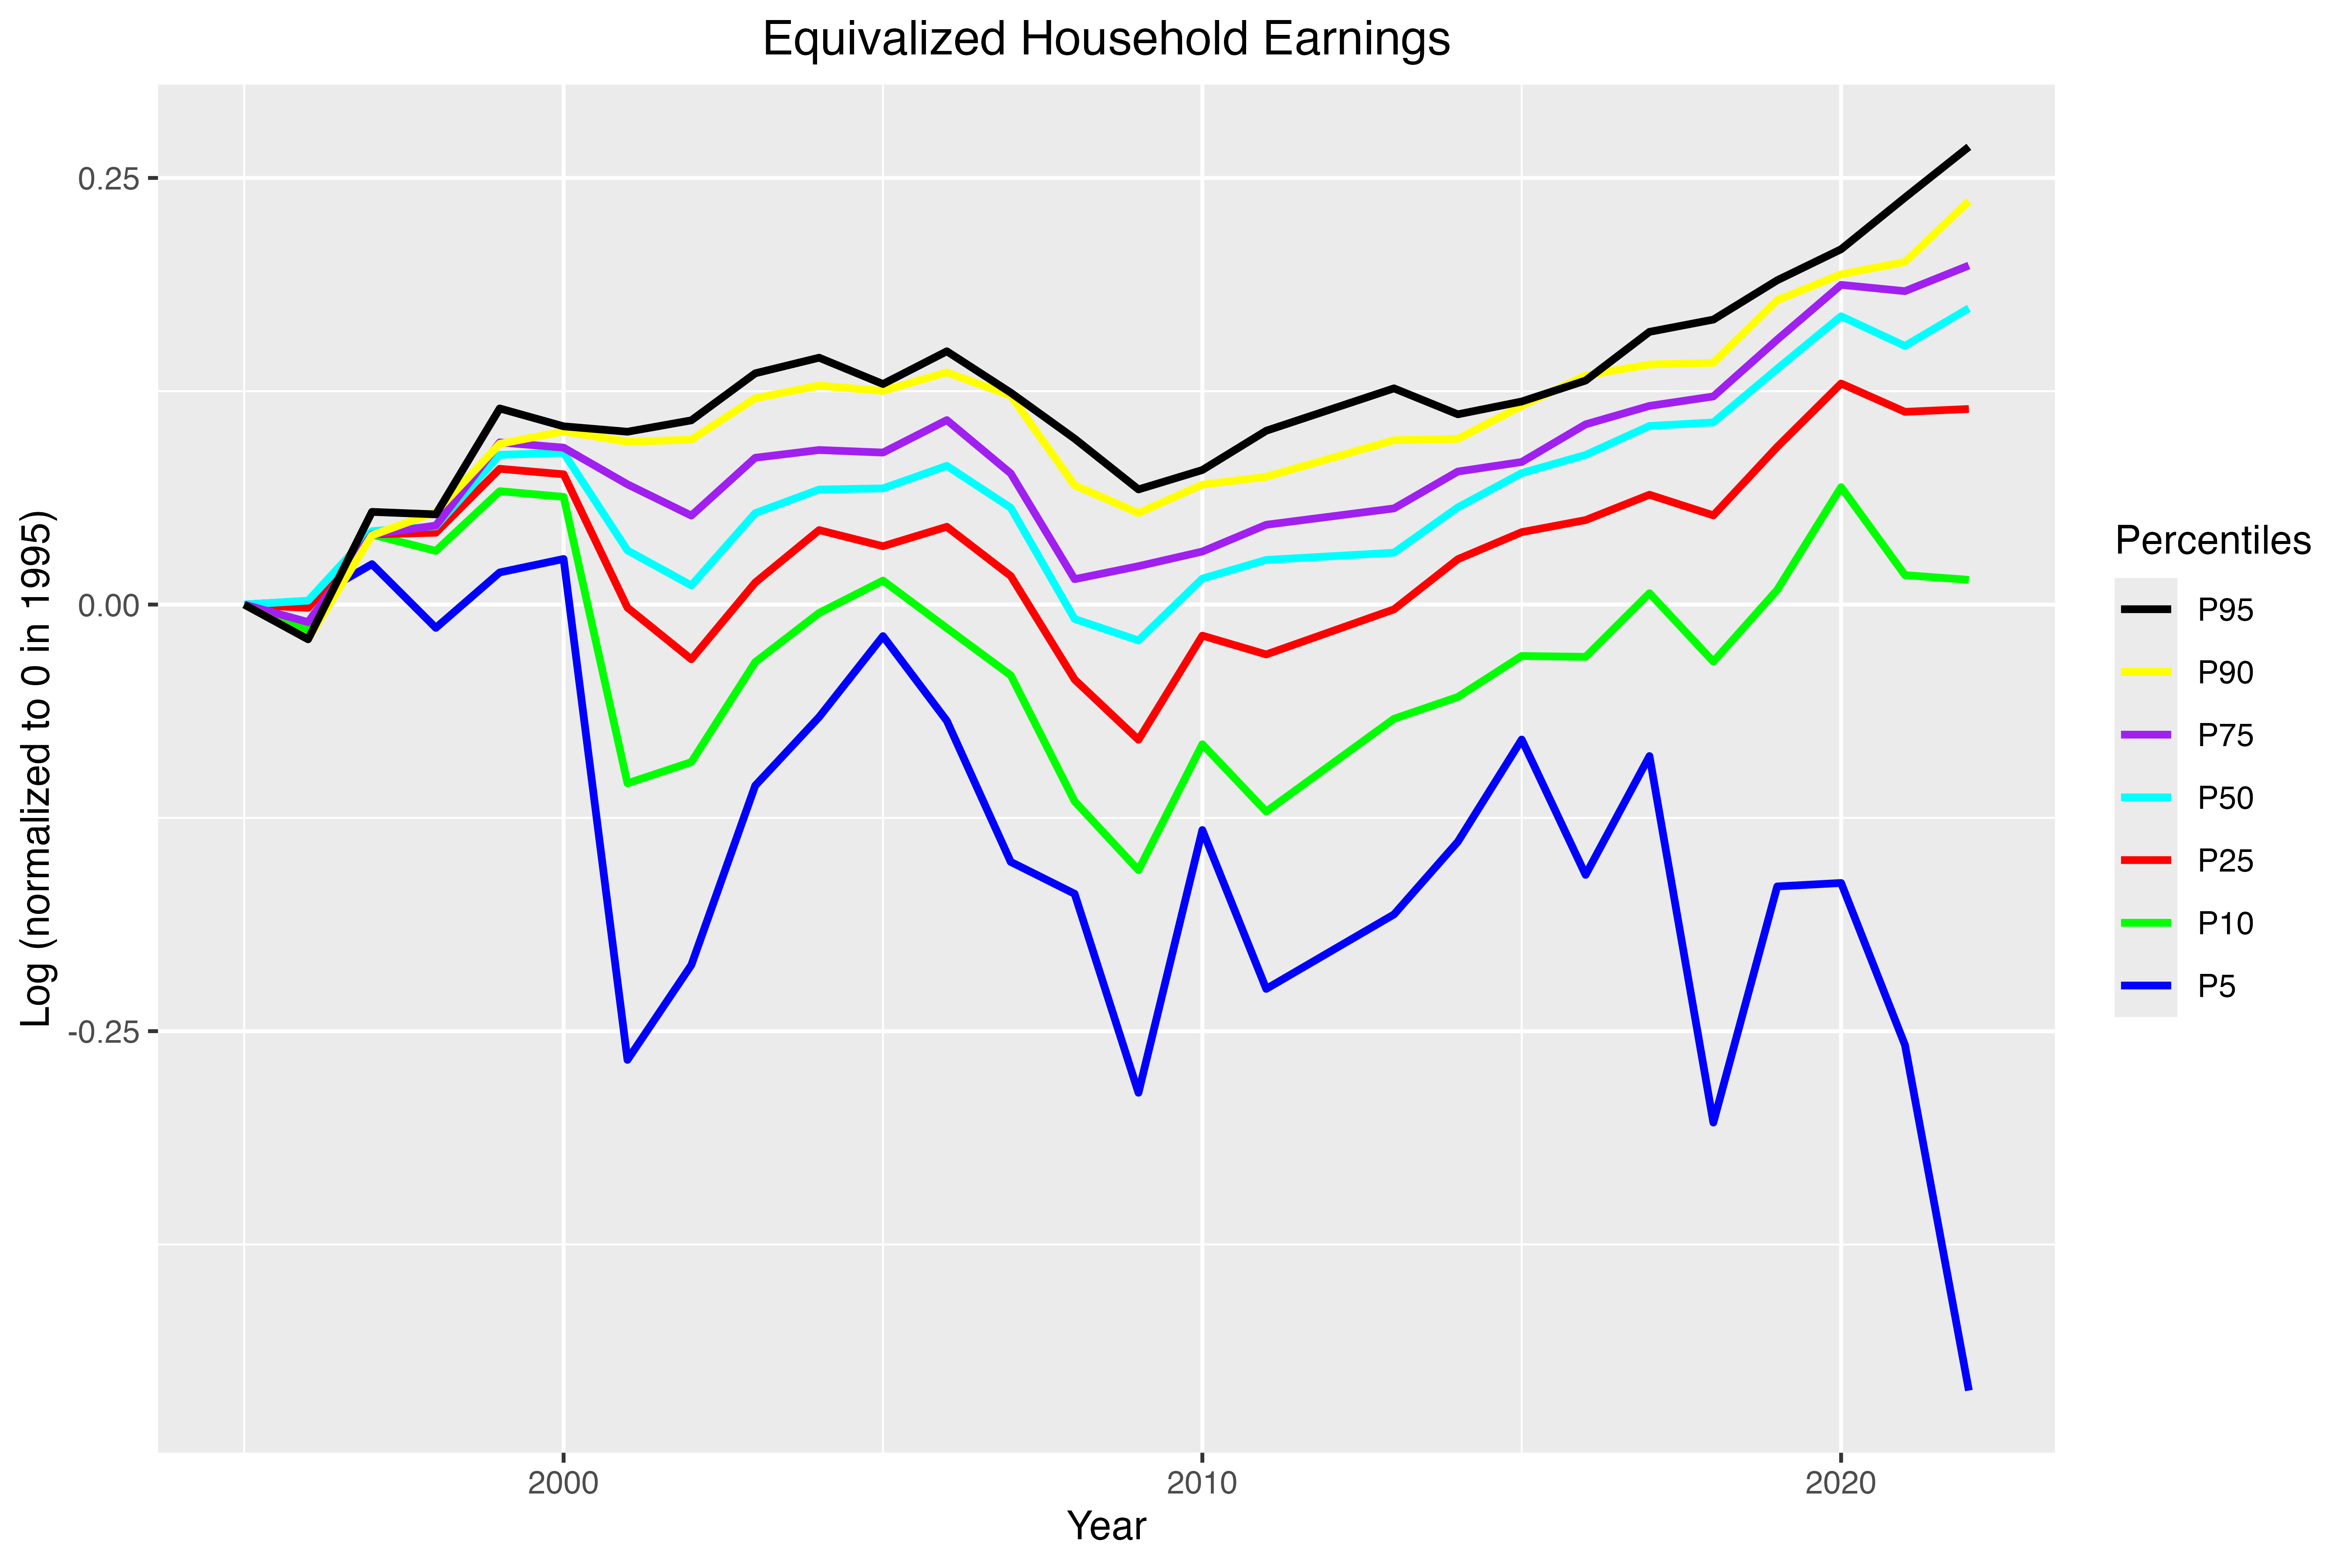
\includegraphics[width=0.95\textwidth]{figures/Fig_2/Fig_2_percentiles_a1995.png}
    \caption{Percentiles of the Household Earnings Distribution}
    \label{fig:earnings_inequality_cyclic}
\end{figure}

Figure \ref{fig:earnings_inequality} plots four measures of dispersion in household earnings: variance of log, Gini coefficient, P50-P10 ratio, and P90-P50 ratio.
Though all measures of dispersion have increased since 1981, there are some minor differences in their dynamics.
The top right variance and the bottom left P50-P10 ratio track each other extremely closely, both spikes around 2000 Dot-com bubble and remain relatively steady after that.
The Gini coefficient in the top right panel shows a steady increase from 0.29 in 1981 to 0.36 in 2023, indicating that earnings inequality has risen over the past four decades.
The bottom right P90-P50 ratio is the most interesting one, it also shows a spike around 2000, but it has been decreasing since then, indicating that the earnings of the top 10\% have not been growing as fast as the median earnings after 2000.
It is worth noting that though the dispersion of earnings has been drastically increasing visually since 1981, the growth of these measurements is actually quite modest compared to other countries, such as the US.
The Gini coefficient for household earnings in Taiwan has increased only 7 log points during the past four decades, while Bourguignon, Fournier, \& Gurgand (\citeyear{TW_stable_dist}) showed that in the US, the Gini coefficient for household earnings has increased roughly 30 log points from 1968 to 2005.



\subsection{Cyclical Dynamics of Earnings Inequality}

Figure \ref{fig:earnings_inequality_cyclic} shows the trend in percentiles at different points in the distribution of household earnings from 1995 to 2023. The log earnings were normalized to 0 in 1995. Therefore, the y-axis shows the percentage change in earnings (as log points) relative to 1995.
Here, I choose to show the result after and normalize it to 1995. The full results from 1981 to 2023 are in the appendix \ref{sec:appendix_cyclical_dynamics} where Figure \ref{fig:appendix_cyclic_earnings_1981} normalized to 1981 and \ref{fig:appendix_cyclic_earnings_1995} normalized to 1995. 
The reason for this choice is that all the percentiles grew over 100 log points from 1981 to 1995; that is, the earnings of all households have tripled since 1981.
This finding coincides with Bourguignon, Fournier, \& Gurgand (\citeyear{TW_stable_dist}) that before 1994, the income of Taiwanese households was in both a fast developing and stable environment.
Therefore, putting years before 1995 in the main figure could dilute the interpretation of recent trends, as the rapid growth phase would dominate the visual impression. By focusing on the period after 1995, we can better highlight the cyclical and structural changes in earnings inequality that occurred after Taiwan's high-growth era ended. This approach allows for a more precise analysis of the dynamics relevant to the current policy and economic environment.

We can see the fanning out of the earning distribution over time, especially for the lower percentiles, such as the 5th and 10th percentiles. The bottom 10\% almost did not grow from 1995 to 2023, and the bottom 5\% declined by over 40 log points, even worse than 1990. The decline of P5 after 2000 is particularly striking; this can be attributed to the COVID-19 pandemic, which has disproportionately affected low-income households in Taiwan, as in many other countries.
In contrast, the difference in income growth of the top half distribution is minimal compared to the bottom half and can even neglect the top 5\% and 10\%, who have grown by about 25 log points since 1995. This contributes to the decrease in the P90-P50 ratio shown in the bottom right of Figure \ref{fig:earnings_inequality}.

Inequality tends to widen during the recession, such as the Dot-com bubble in 2000, the Global Financial Crisis in 2008, and the COVID-19 pandemic in 2020. The reason behind this phenomenon is that when facing external shocks, households with higher earnings are more likely to have diversified income sources, such as investments and insurance transfers, which can help them weather economic downturns better than those with lower earnings who rely more on labor income. We can also observe this phenomenon in the percentiles of earnings distribution, where the lower percentiles tend to decline sharply while the upper percentiles remain relatively stable.

\subsection{From Individual to Household Inequality}

\begin{figure}
    \centering
    \begin{subfigure}[t]{0.475\textwidth}
        \centering
        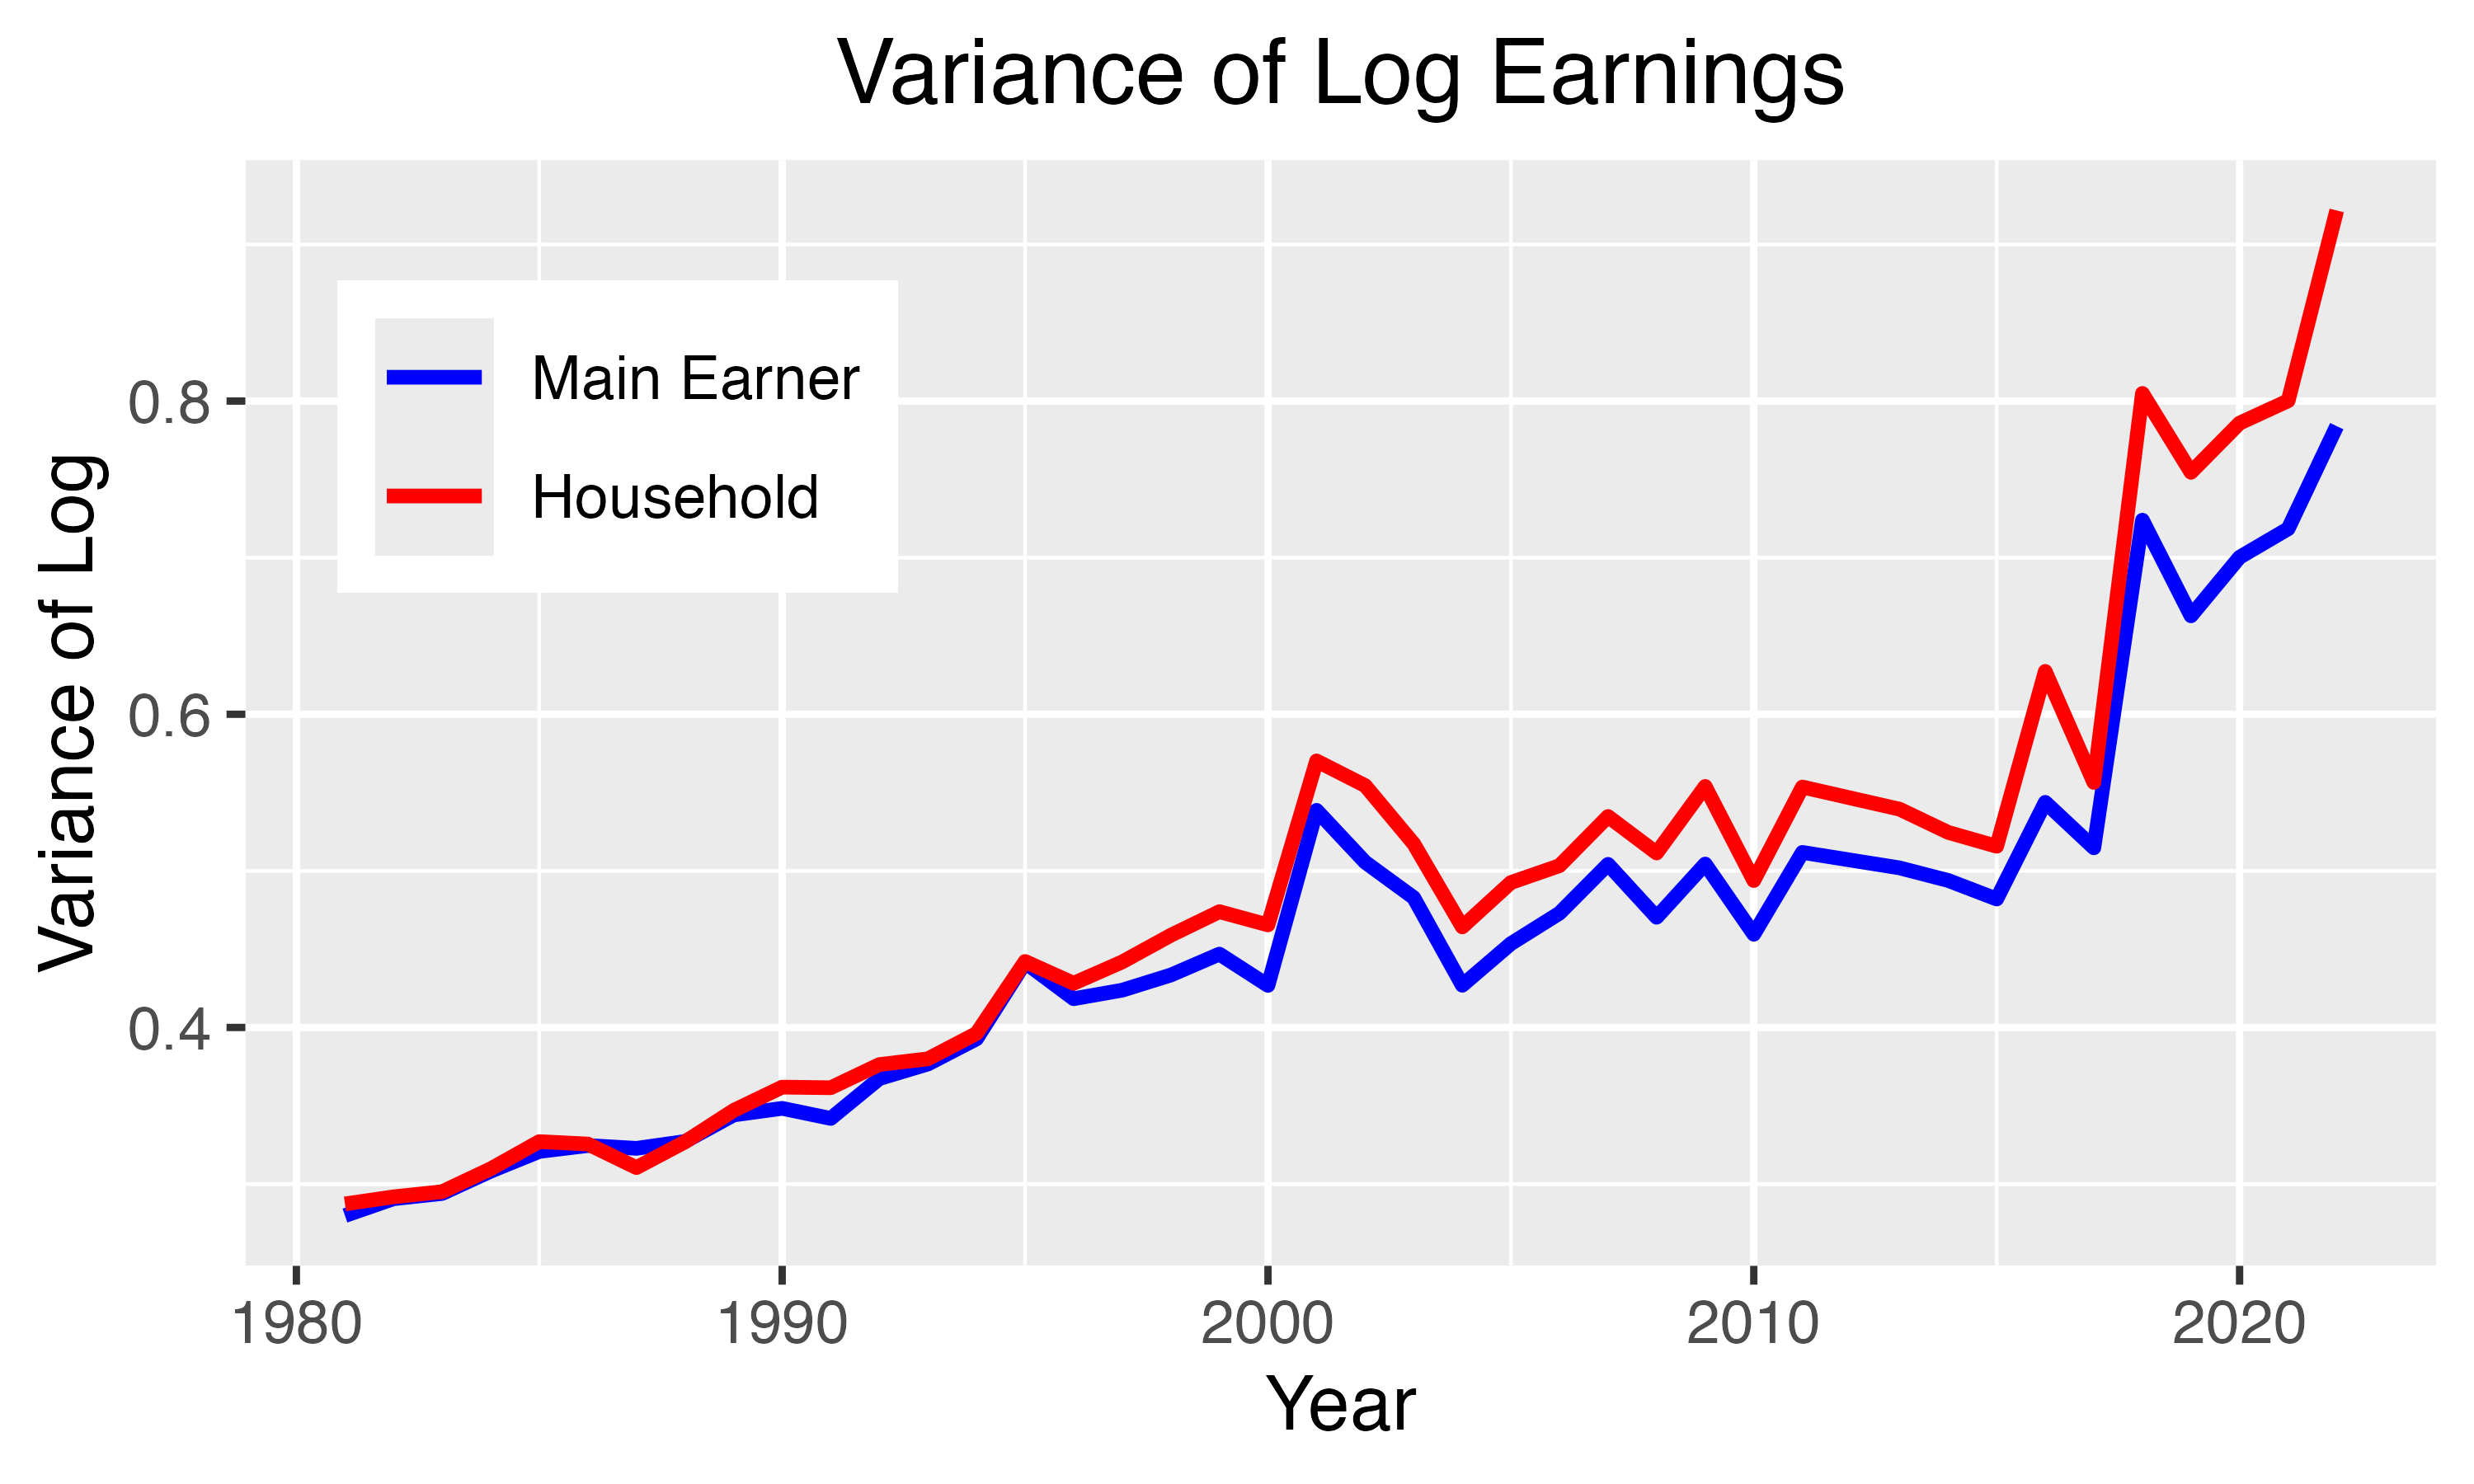
\includegraphics[width=\textwidth]{figures/Fig_3/Fig_3a_Var_indHH.png}
    \end{subfigure}
    \begin{subfigure}[t]{0.475\textwidth}
        \centering
        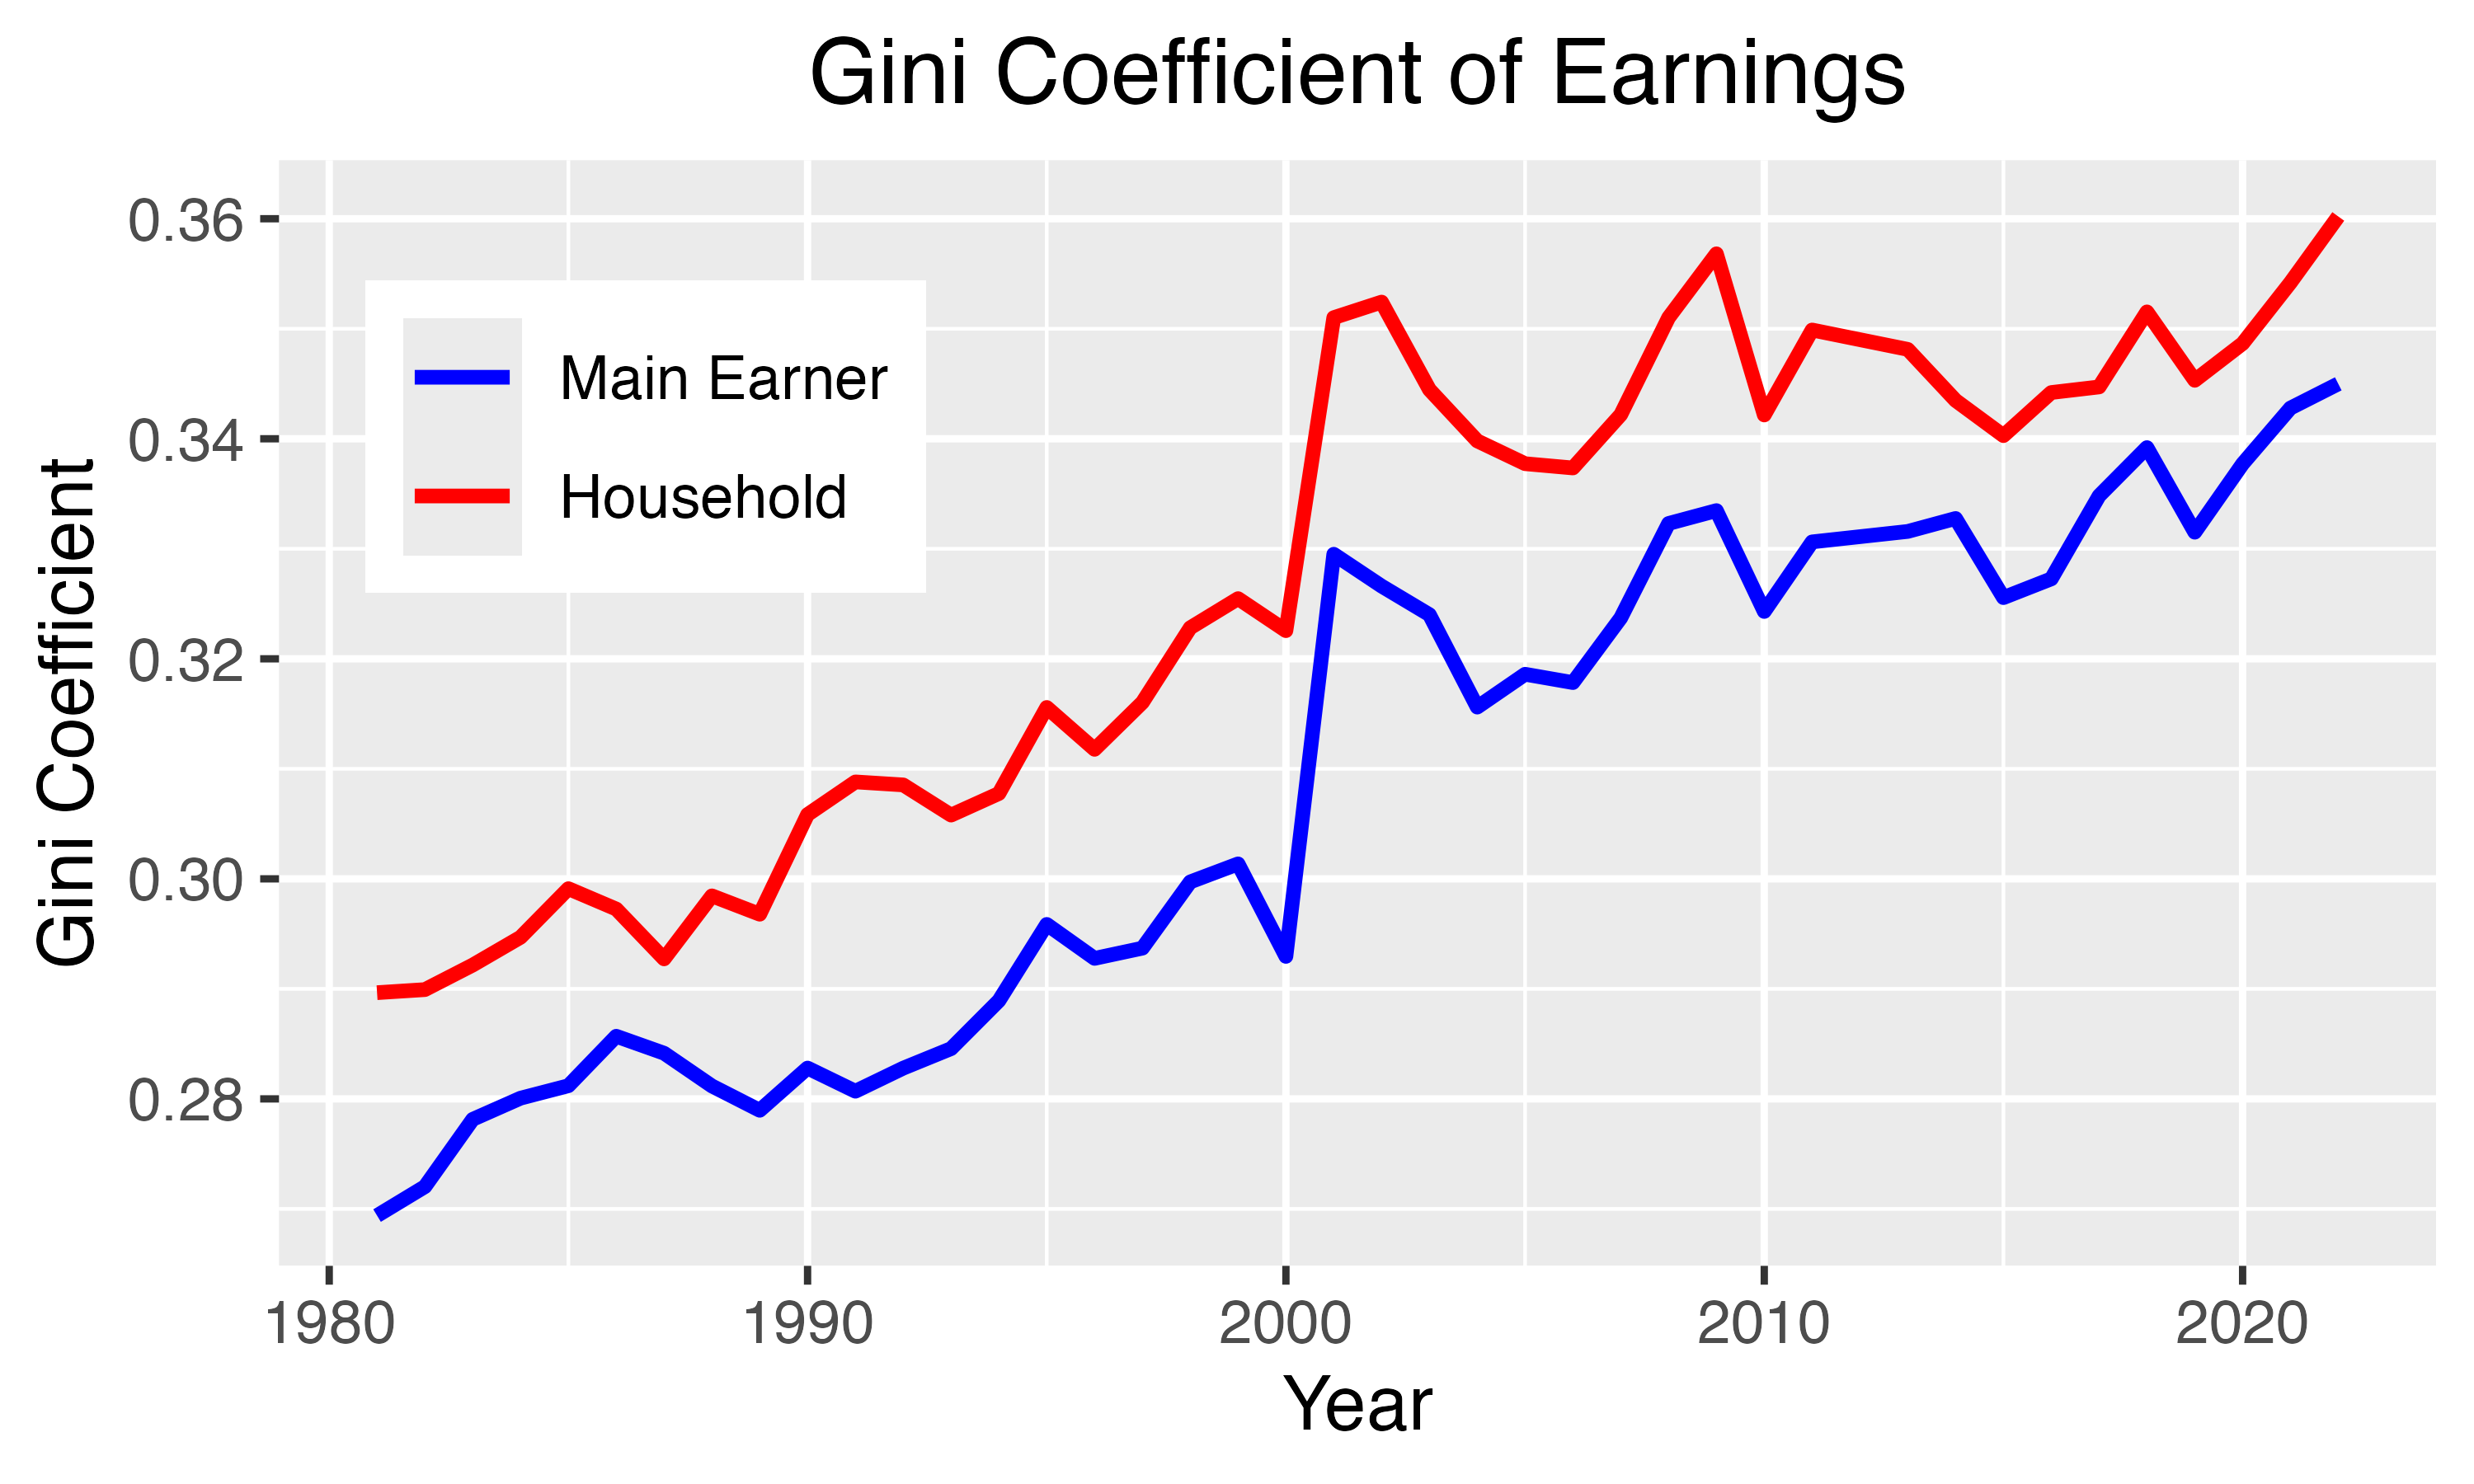
\includegraphics[width=\textwidth]{figures/Fig_3/Fig_3b_Gini_indHH.png}
    \end{subfigure}
    \begin{subfigure}[t]{0.475\textwidth}
        \centering
        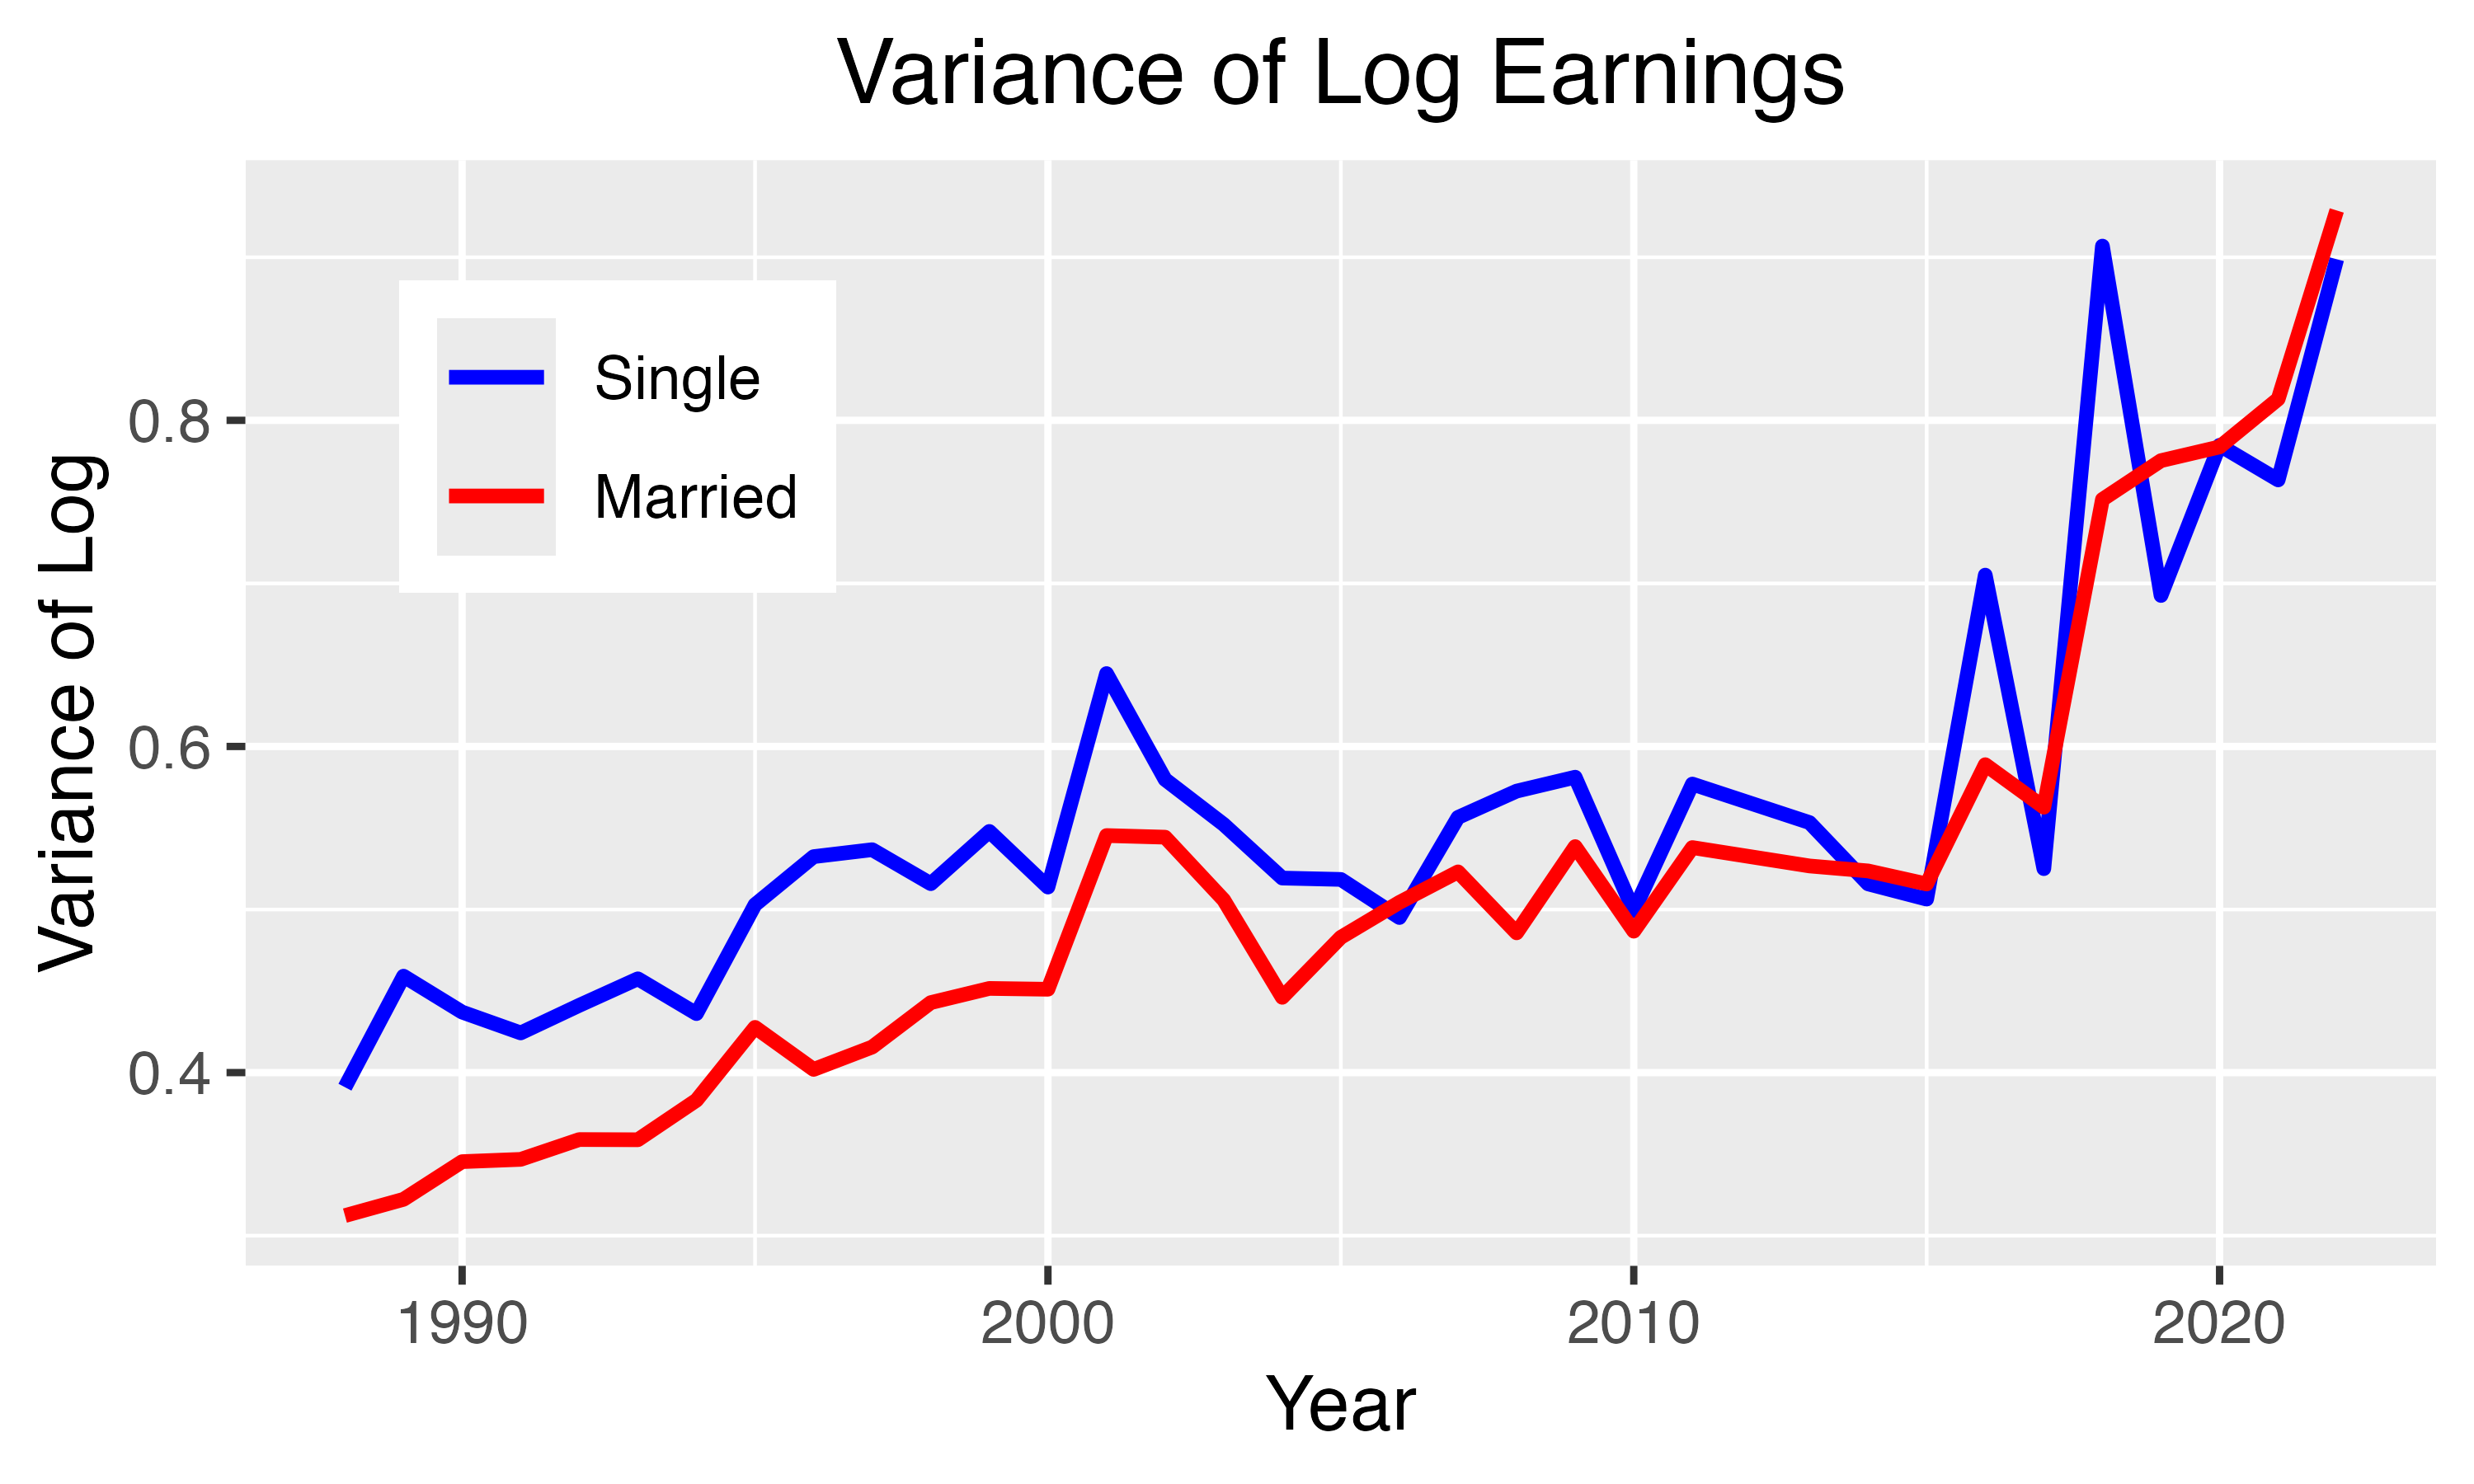
\includegraphics[width=\textwidth]{figures/Fig_3/Fig_3c_Var_single.png}
    \end{subfigure}
    \begin{subfigure}[t]{0.475\textwidth}
        \centering
        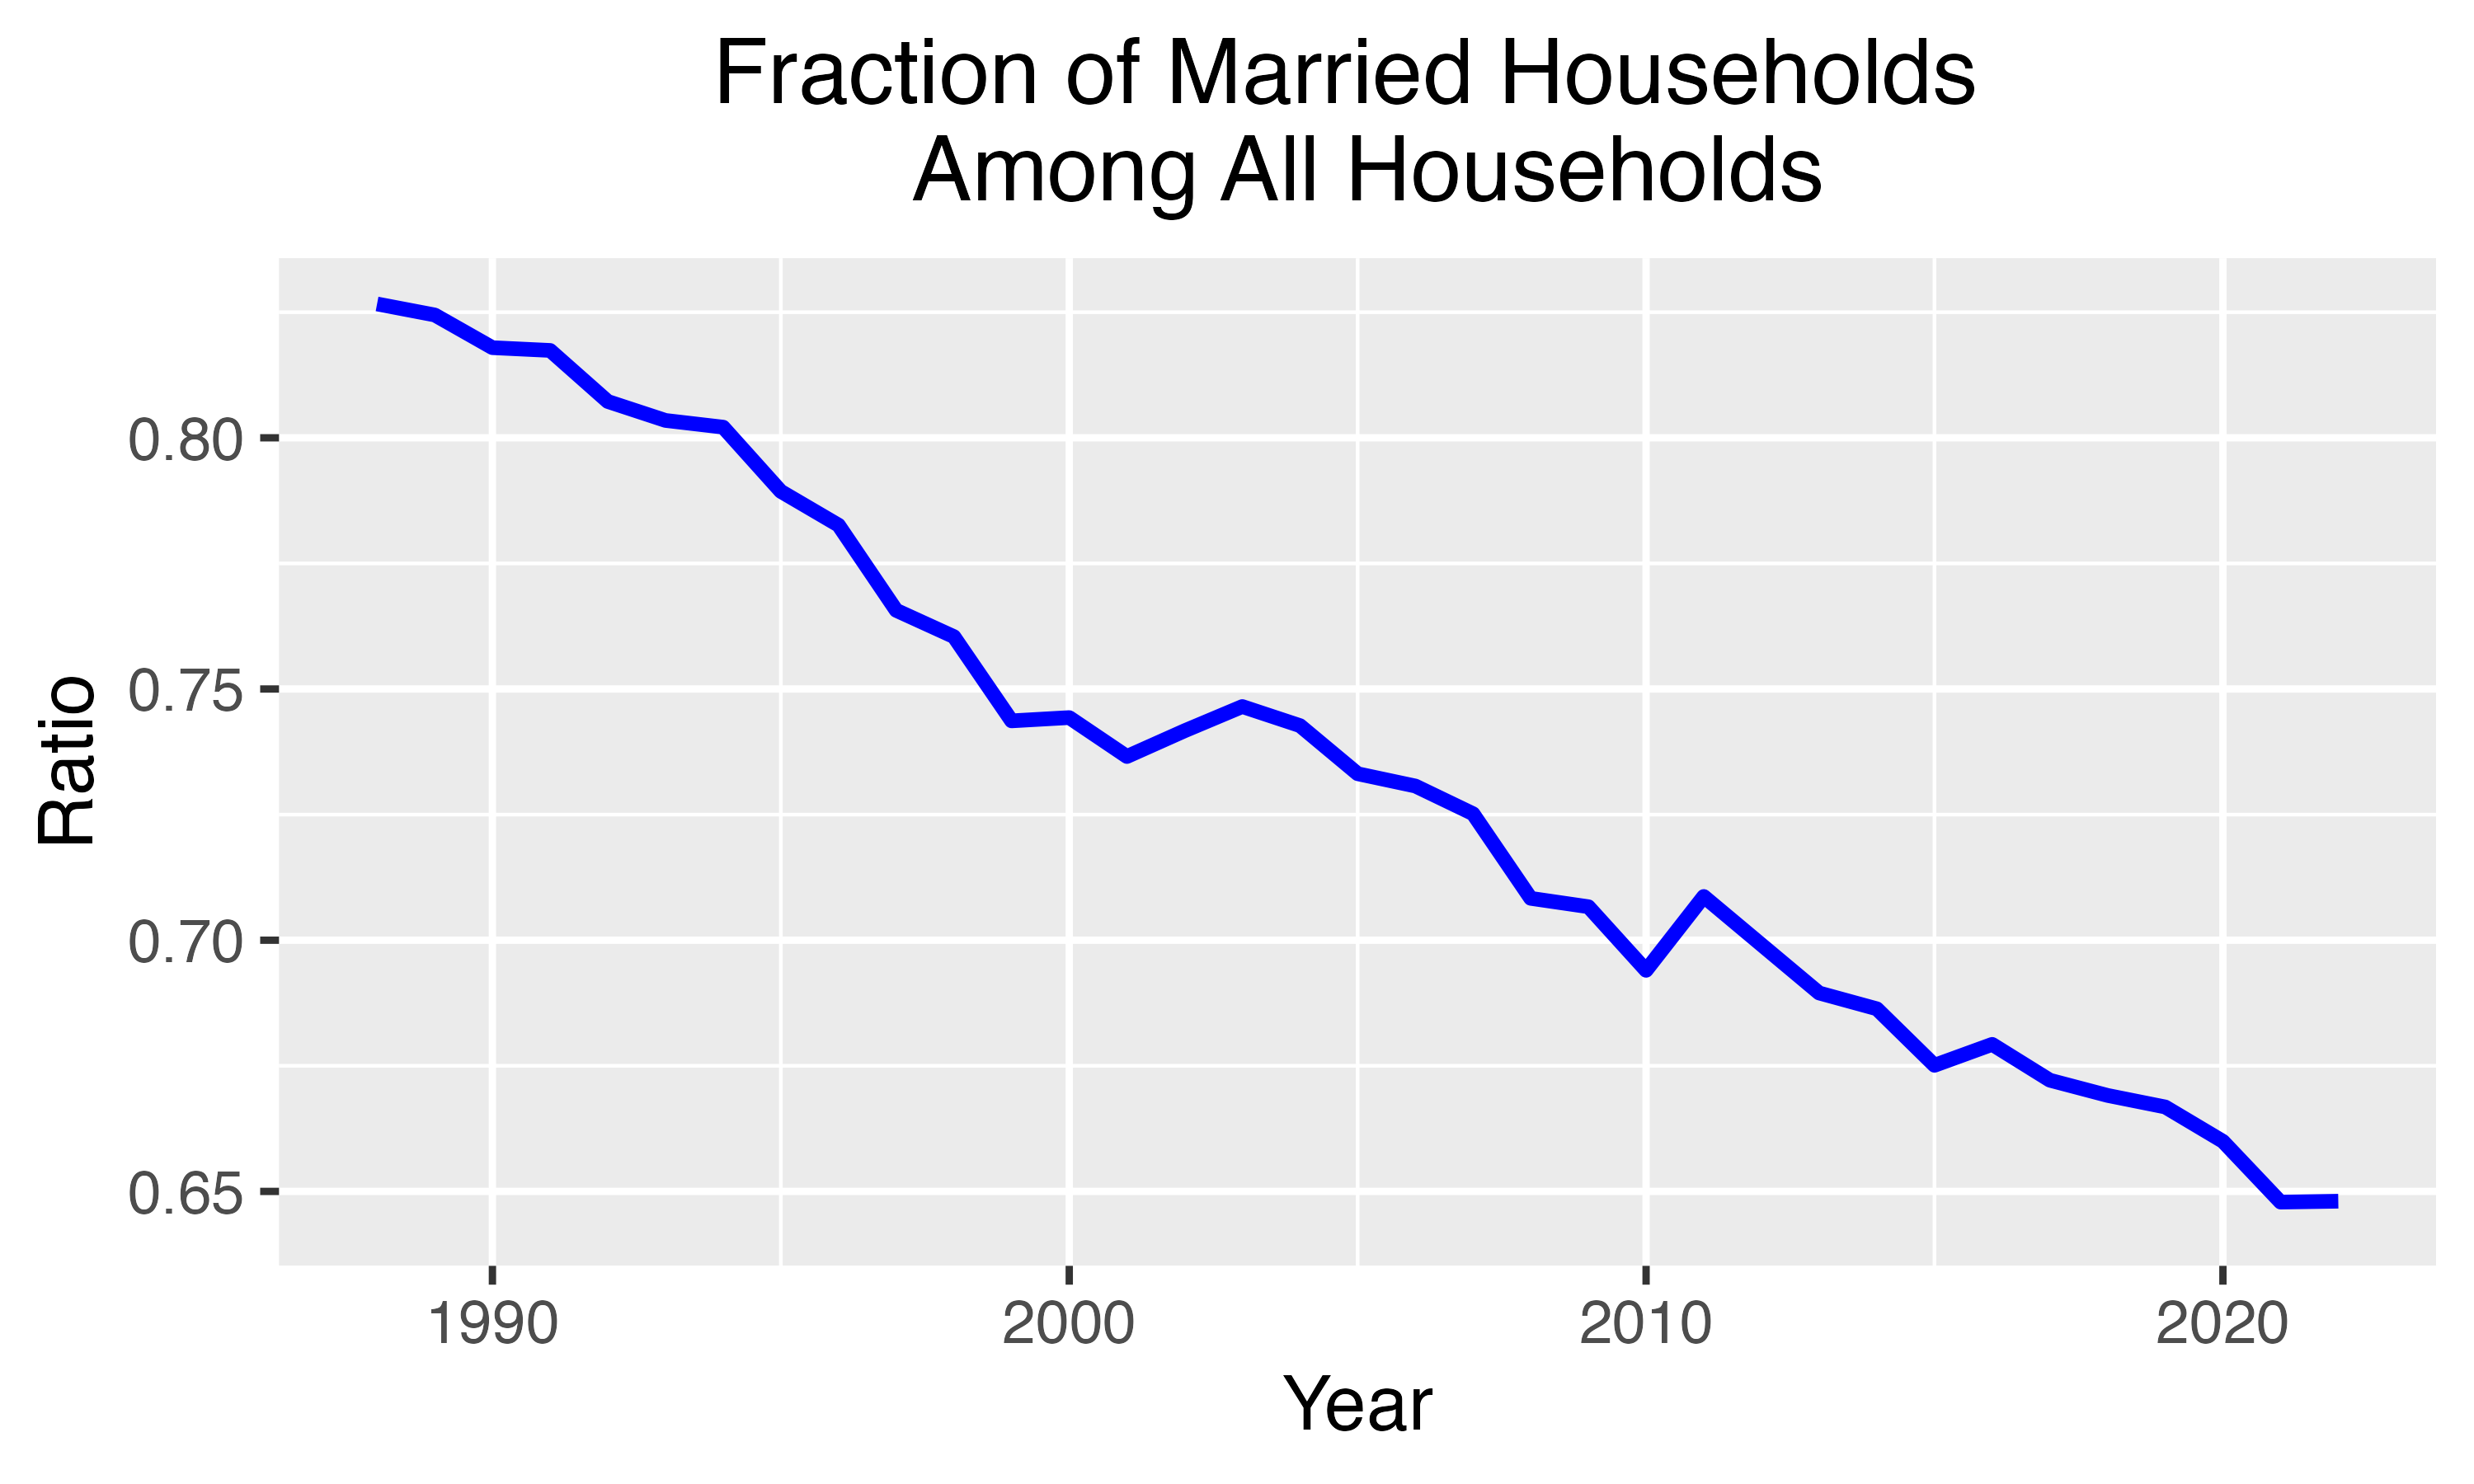
\includegraphics[width=\textwidth]{figures/Fig_3/Fig_3d_married_ratio.png}
    \end{subfigure}
    \begin{subfigure}[t]{0.475\textwidth}
        \centering
        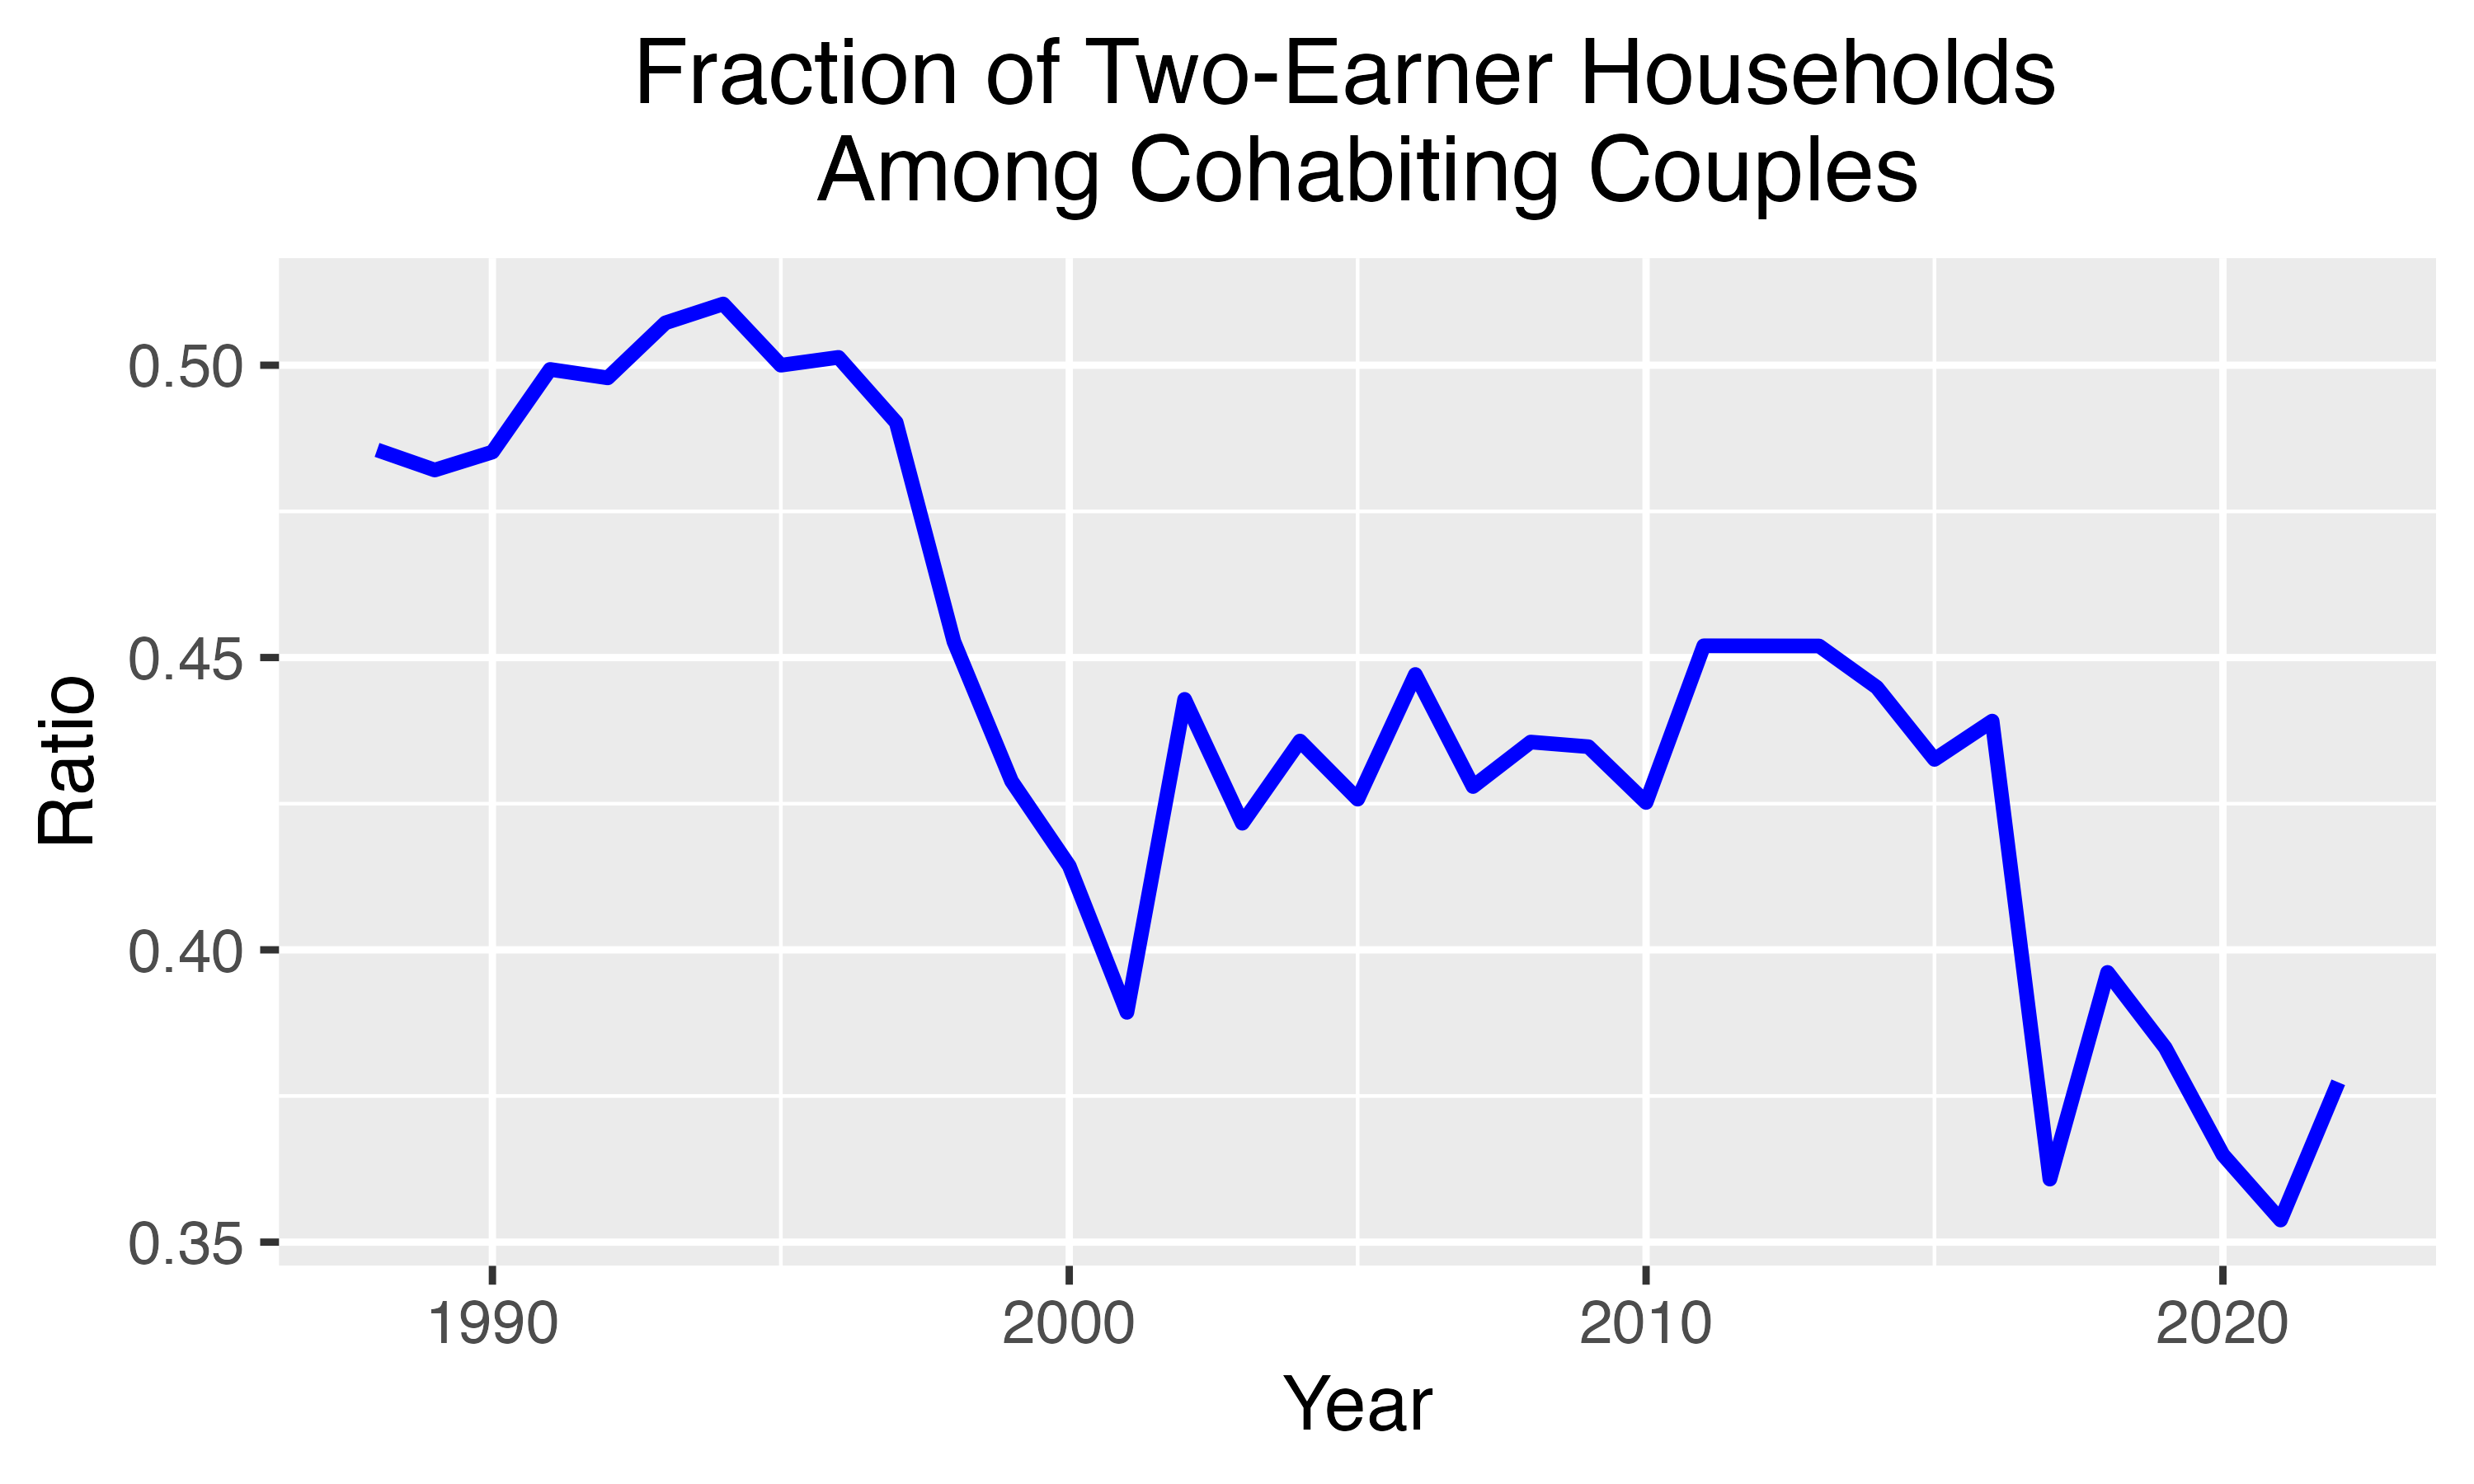
\includegraphics[width=\textwidth]{figures/Fig_3/Fig_3e_two_earner_ratio.png}
    \end{subfigure}
    \begin{subfigure}[t]{0.475\textwidth}
        \centering
        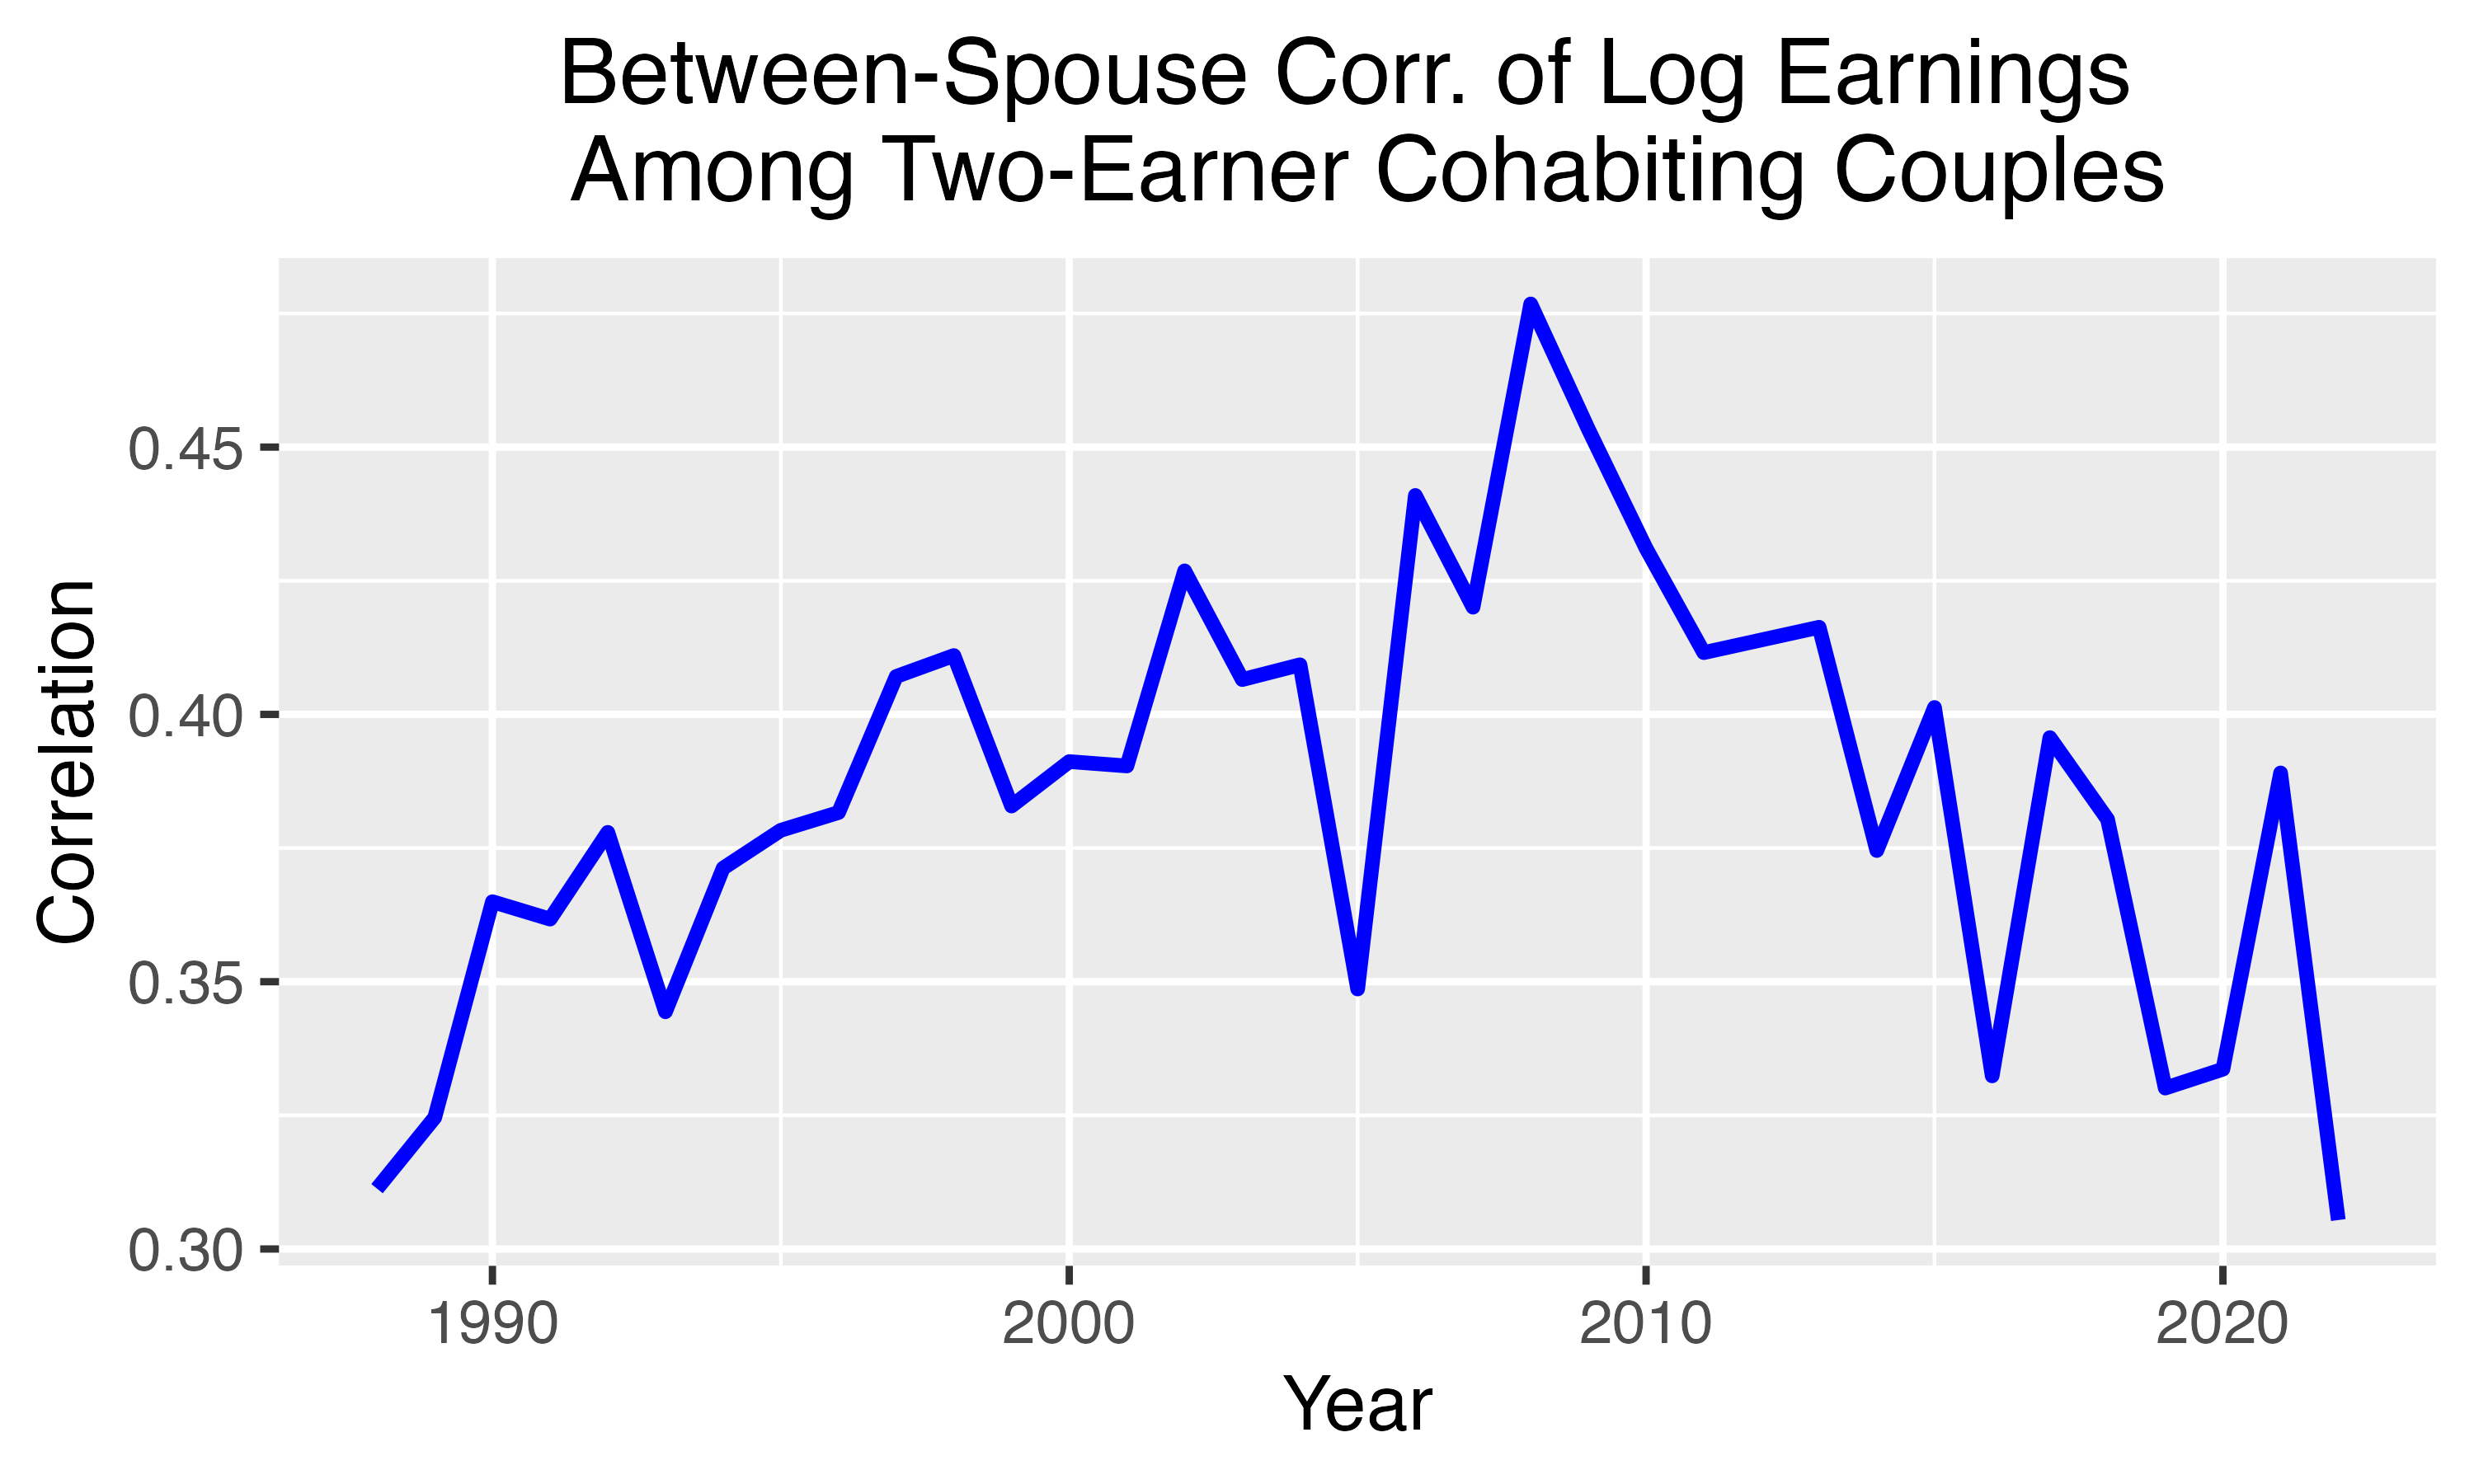
\includegraphics[width=\textwidth]{figures/Fig_3/Fig_3f_correlation.png}
    \end{subfigure}
    \caption{Understanding the role of the Family for Earnings Inequality}
    \label{fig:Indi_to_HH}
\end{figure}

Next, we look at the role of the family in household earnings inequality. The top 2 panels of Figure \ref{fig:Indi_to_HH} show the variance and Gini coefficient of main earner earnings and household earnings. The trend is quite similar, with the household earnings having a slightly higher Gini coefficient. This is a shocking result, as we usually expect the household smoothing the income due to the pooling of resources within families. I do not have a clear answer for this now, but I suspect that the reason is the household structure in SFIE, as shown in the bottom left panel of Figure \ref{fig:Indi_to_HH}, the ratio of two-earner households has been decreasing in our data set, which is not usually the case. The decline in two-earner households we observe can be due to higher-income couples tending to split up their household ID, which can avoid some housing and land tax.

The middle two panels of Figure \ref{fig:Indi_to_HH} show the relation between single and married households. The decreasing fraction of married households contributes to the smaller inequality gap between married and single households. The bottom right panel shows the between-spouse earnings correlation among two-earner cohabiting households, which I also do not know how to interpret now. Initially, I expect the correlation to increase over time, as the two-earner households are more likely to be from the same educational background and have similar earnings. However, the correlation has decreased since 2008, which is the opposite of what I expected. This could also be due to the household structure we discussed above, as the two-earner households that split up would be discarded in our correlation calculation.

\subsection{Private Transfers and Asset Income}

\begin{figure}
    \centering
    \begin{subfigure}[t]{0.475\textwidth}
        \centering
        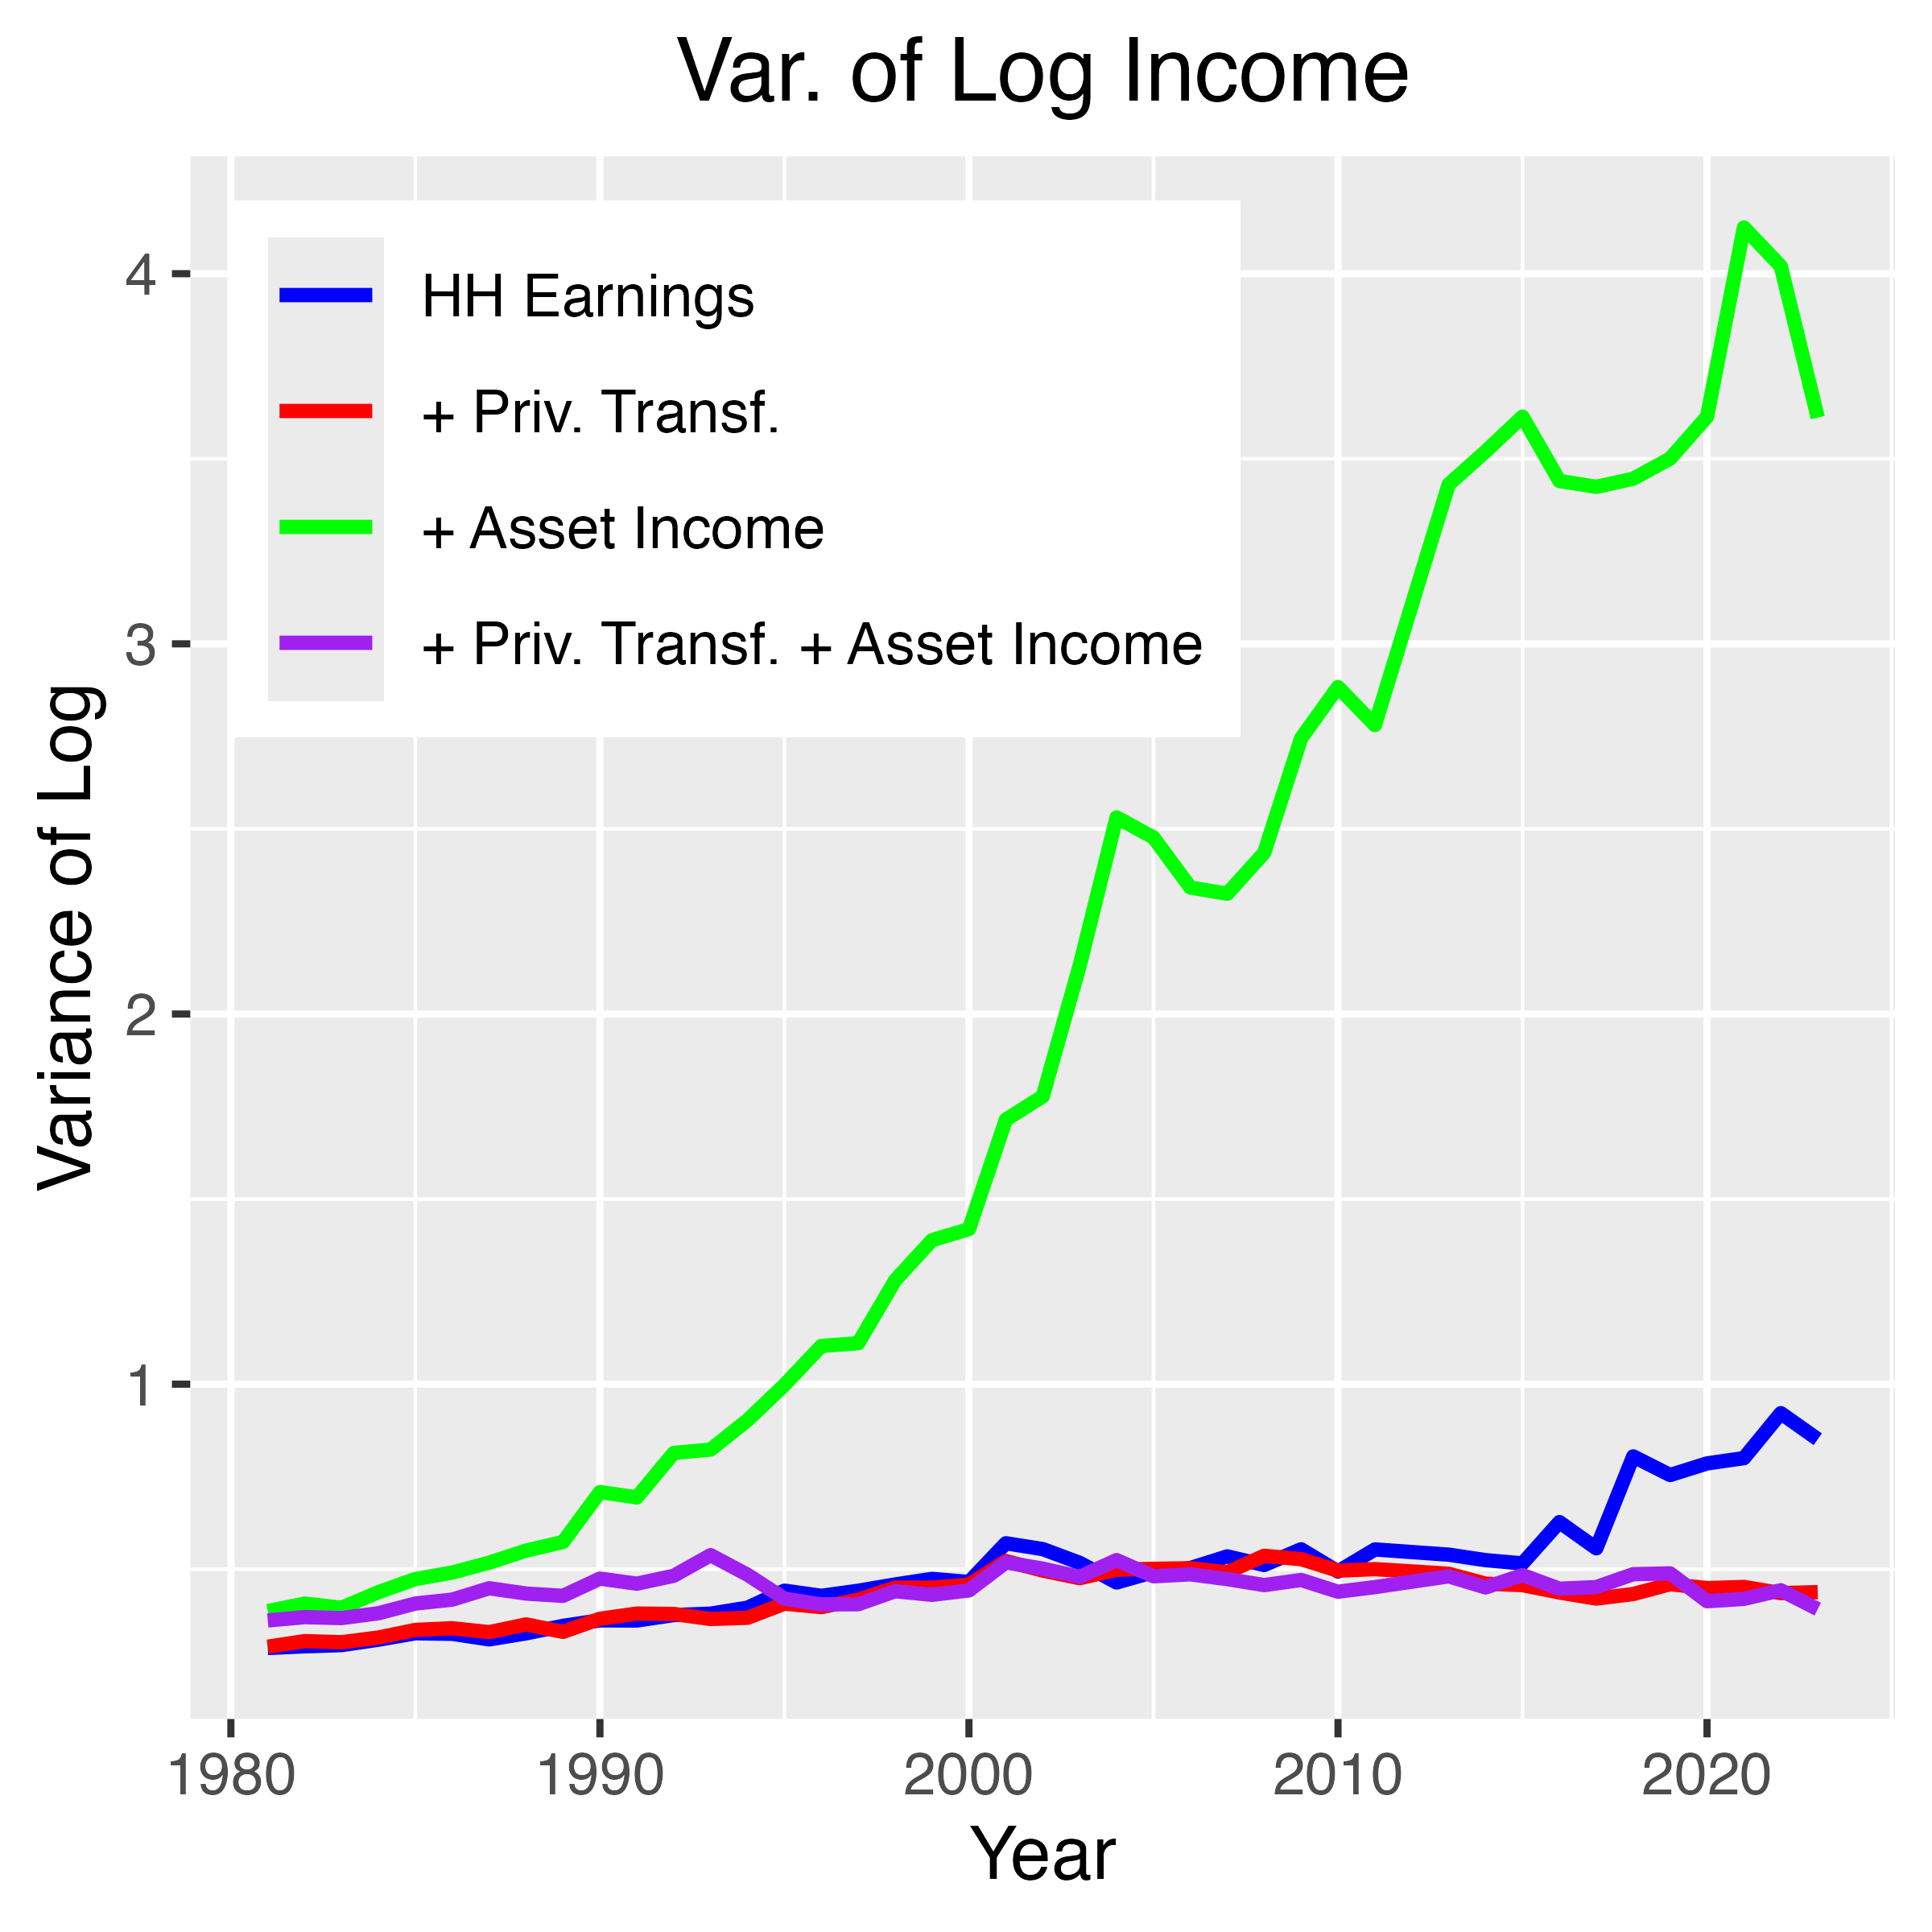
\includegraphics[width=\textwidth]{figures/Fig_4/Fig_4a_Var_inc.png}
    \end{subfigure}
    \begin{subfigure}[t]{0.475\textwidth}
        \centering
        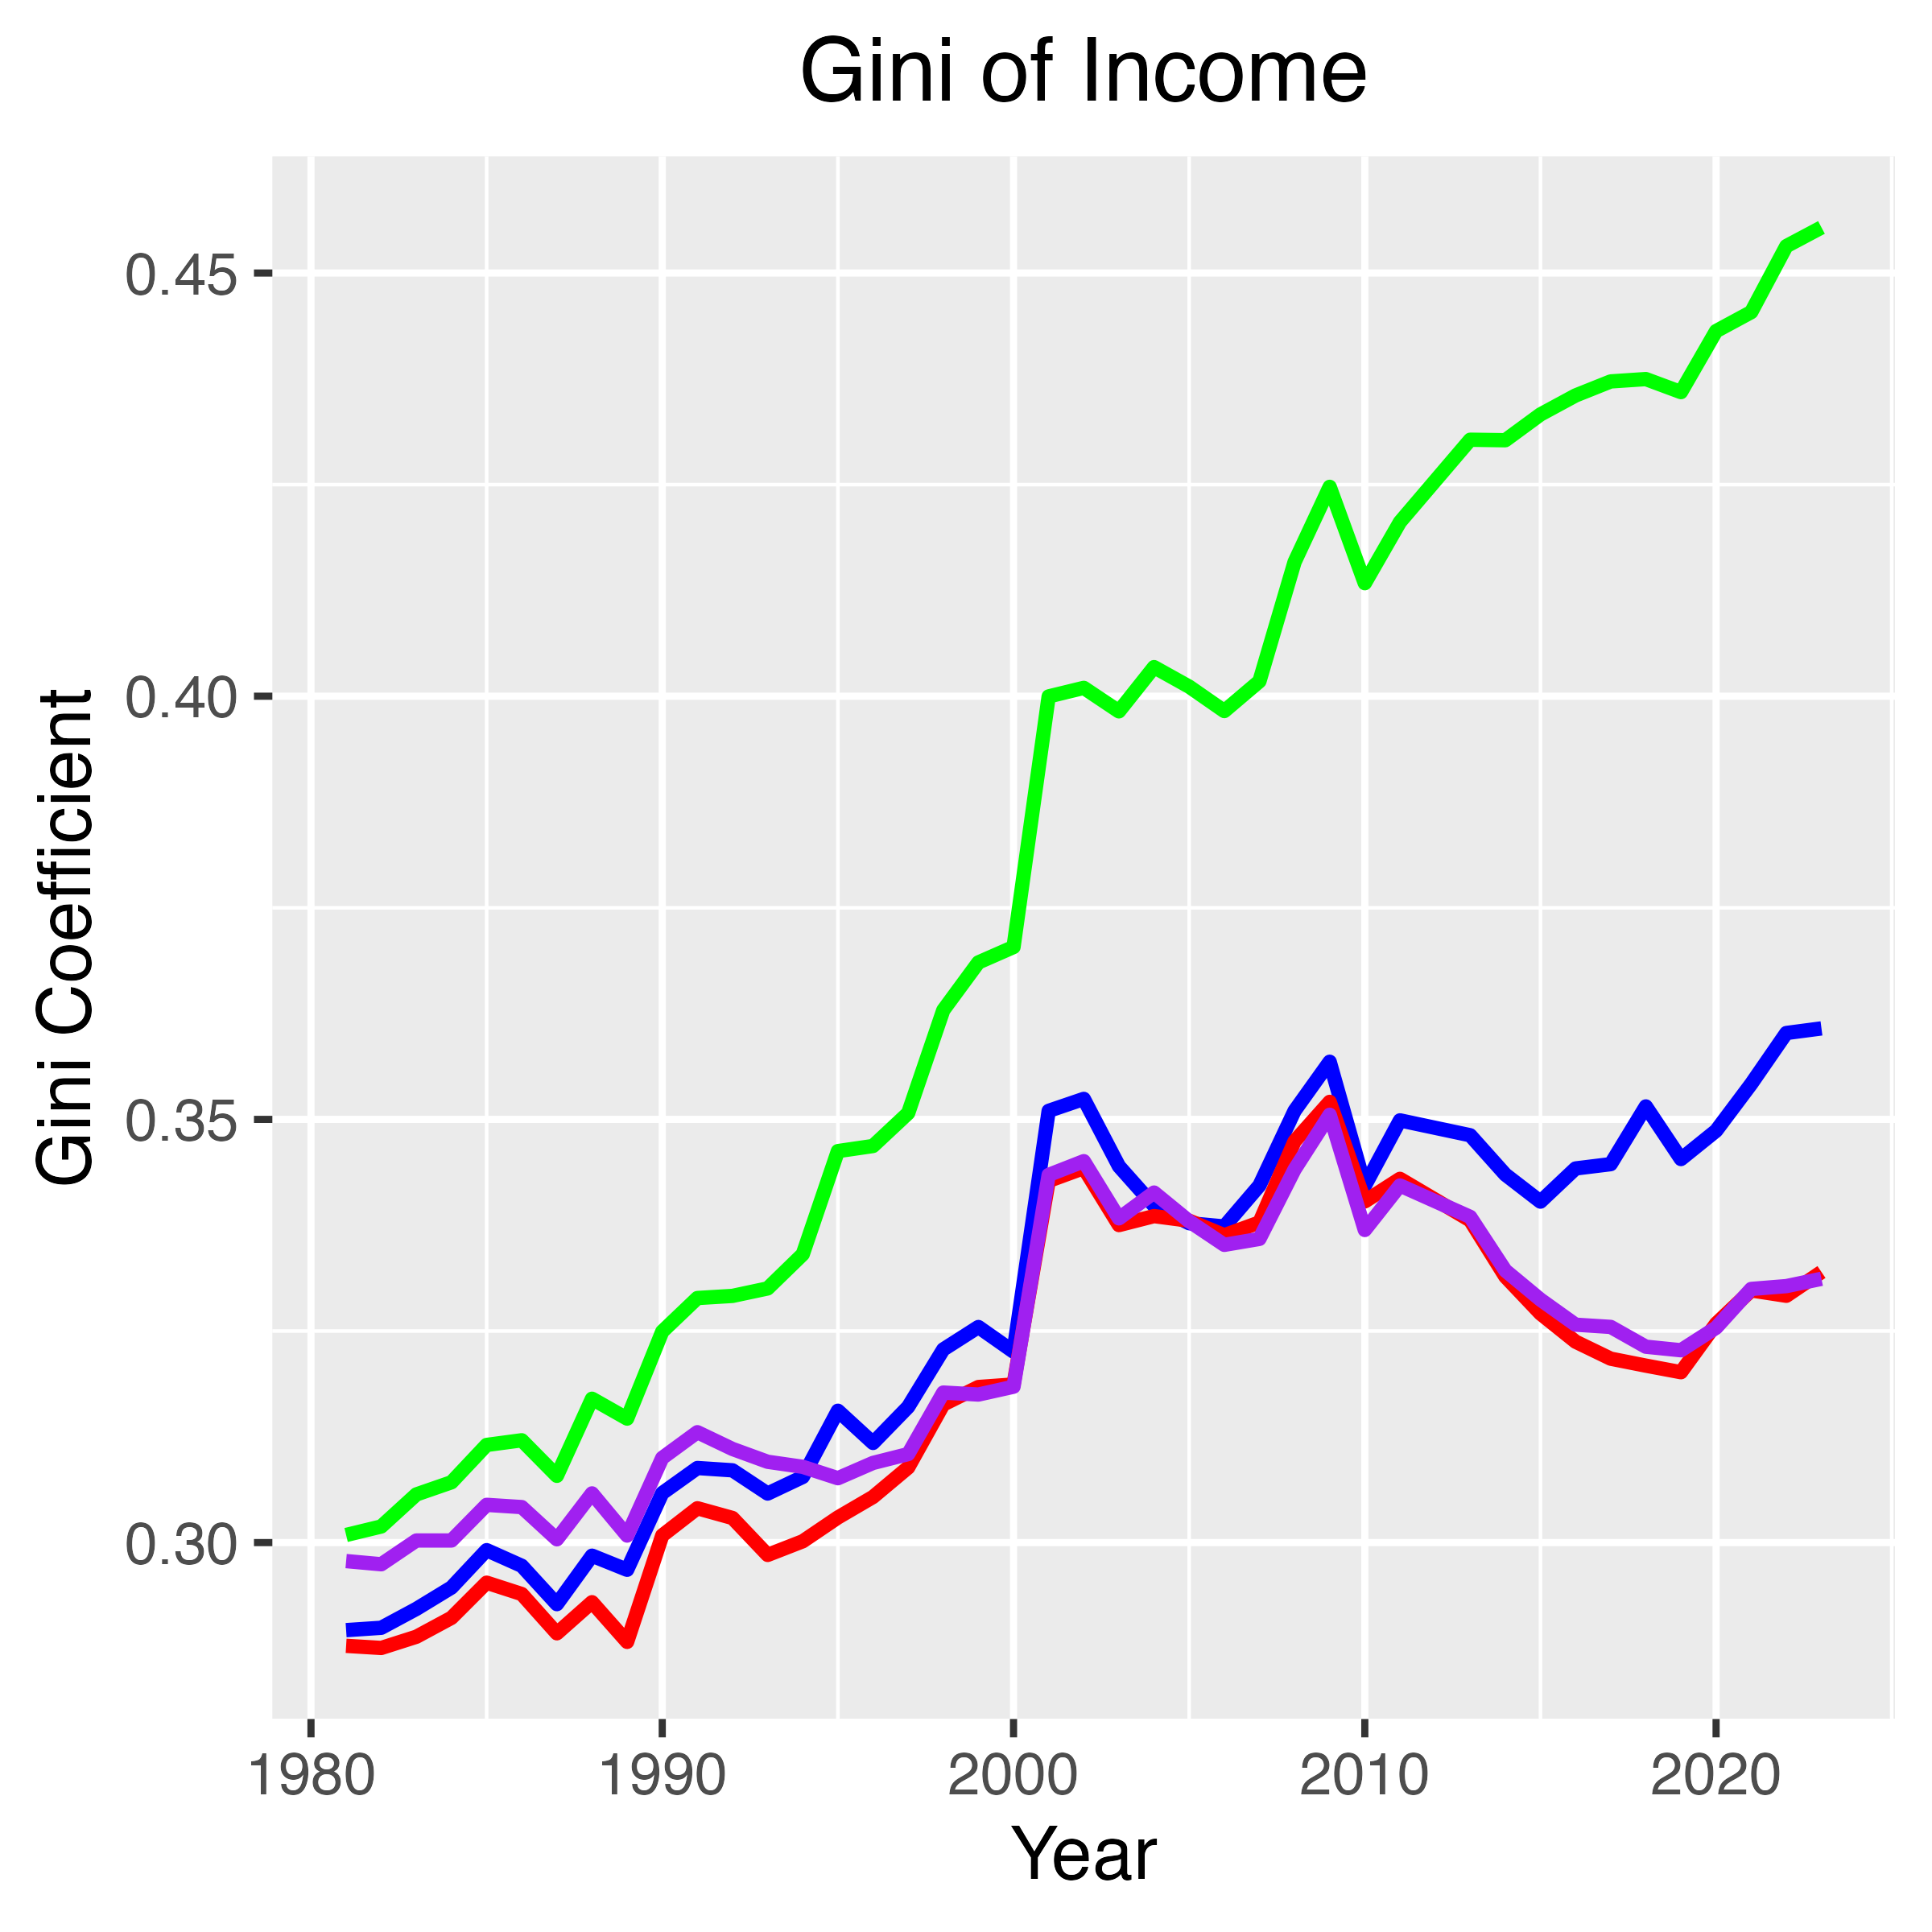
\includegraphics[width=\textwidth]{figures/Fig_4/Fig_4b_Gini_inc.png}
    \end{subfigure}
    \begin{subfigure}[t]{0.475\textwidth}
        \centering
        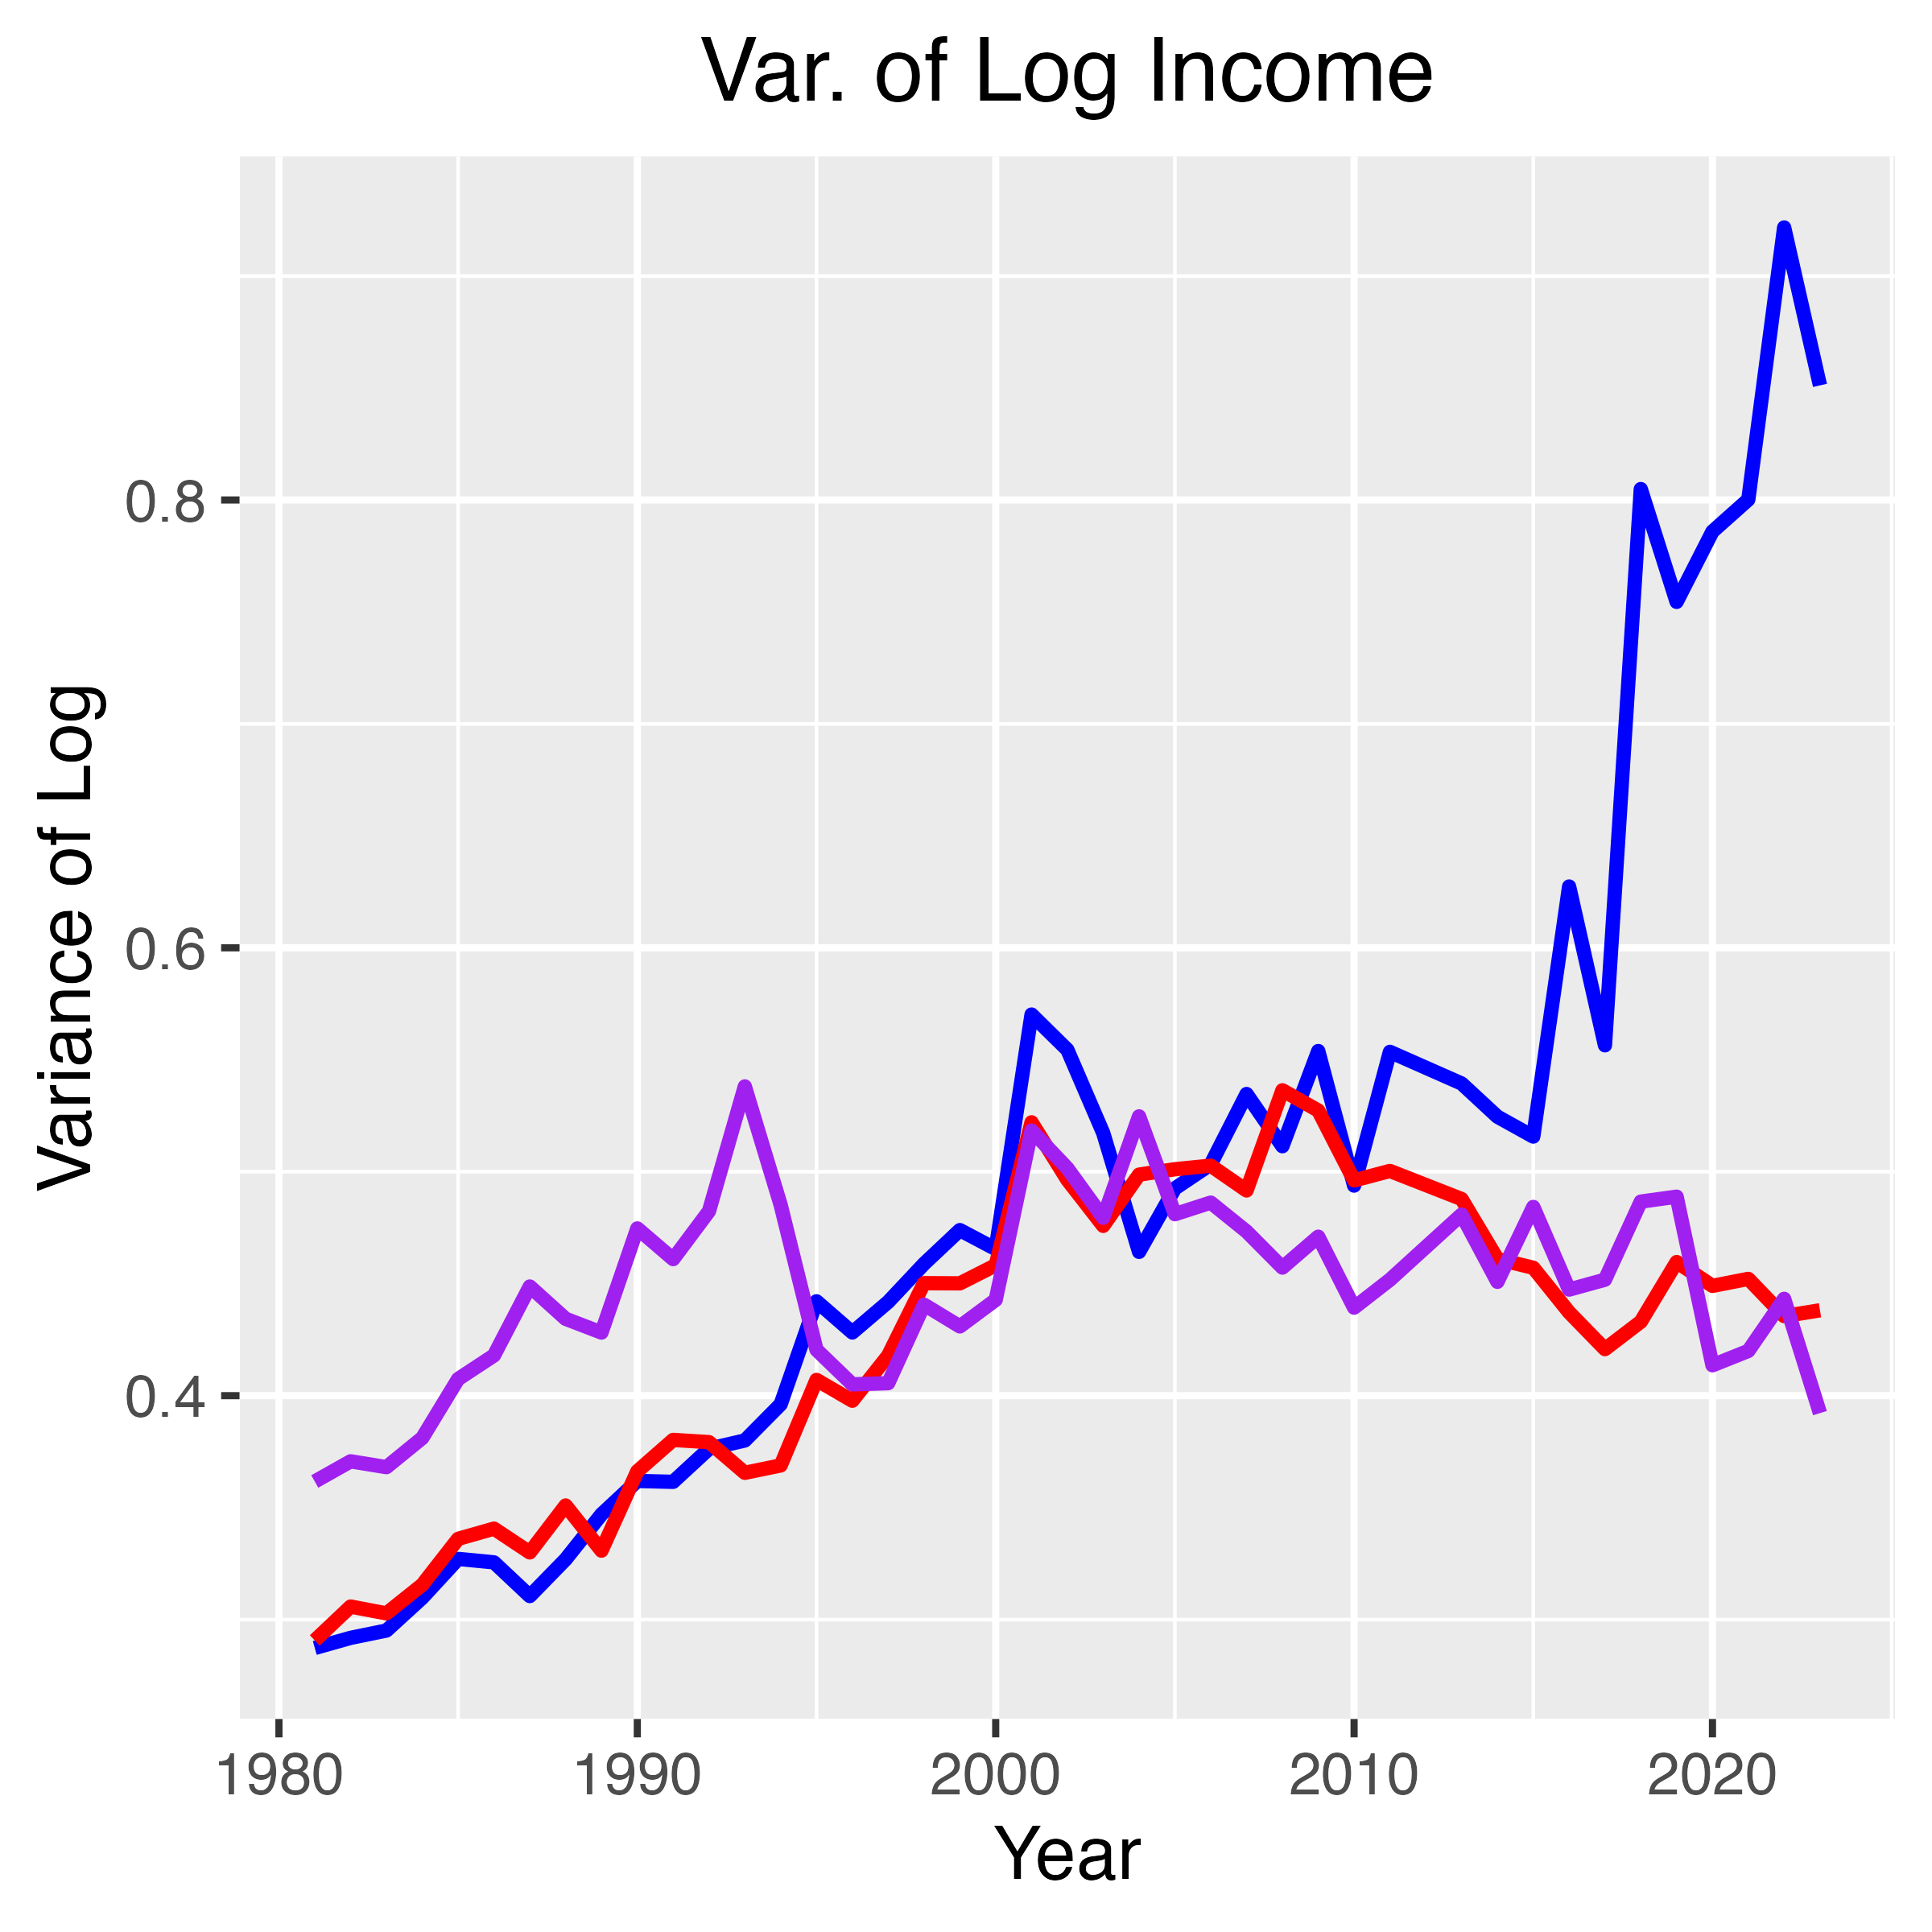
\includegraphics[width=\textwidth]{figures/Fig_4/Fig_4c_Var_inc.png}
    \end{subfigure}
    \begin{subfigure}[t]{0.475\textwidth}
        \centering
        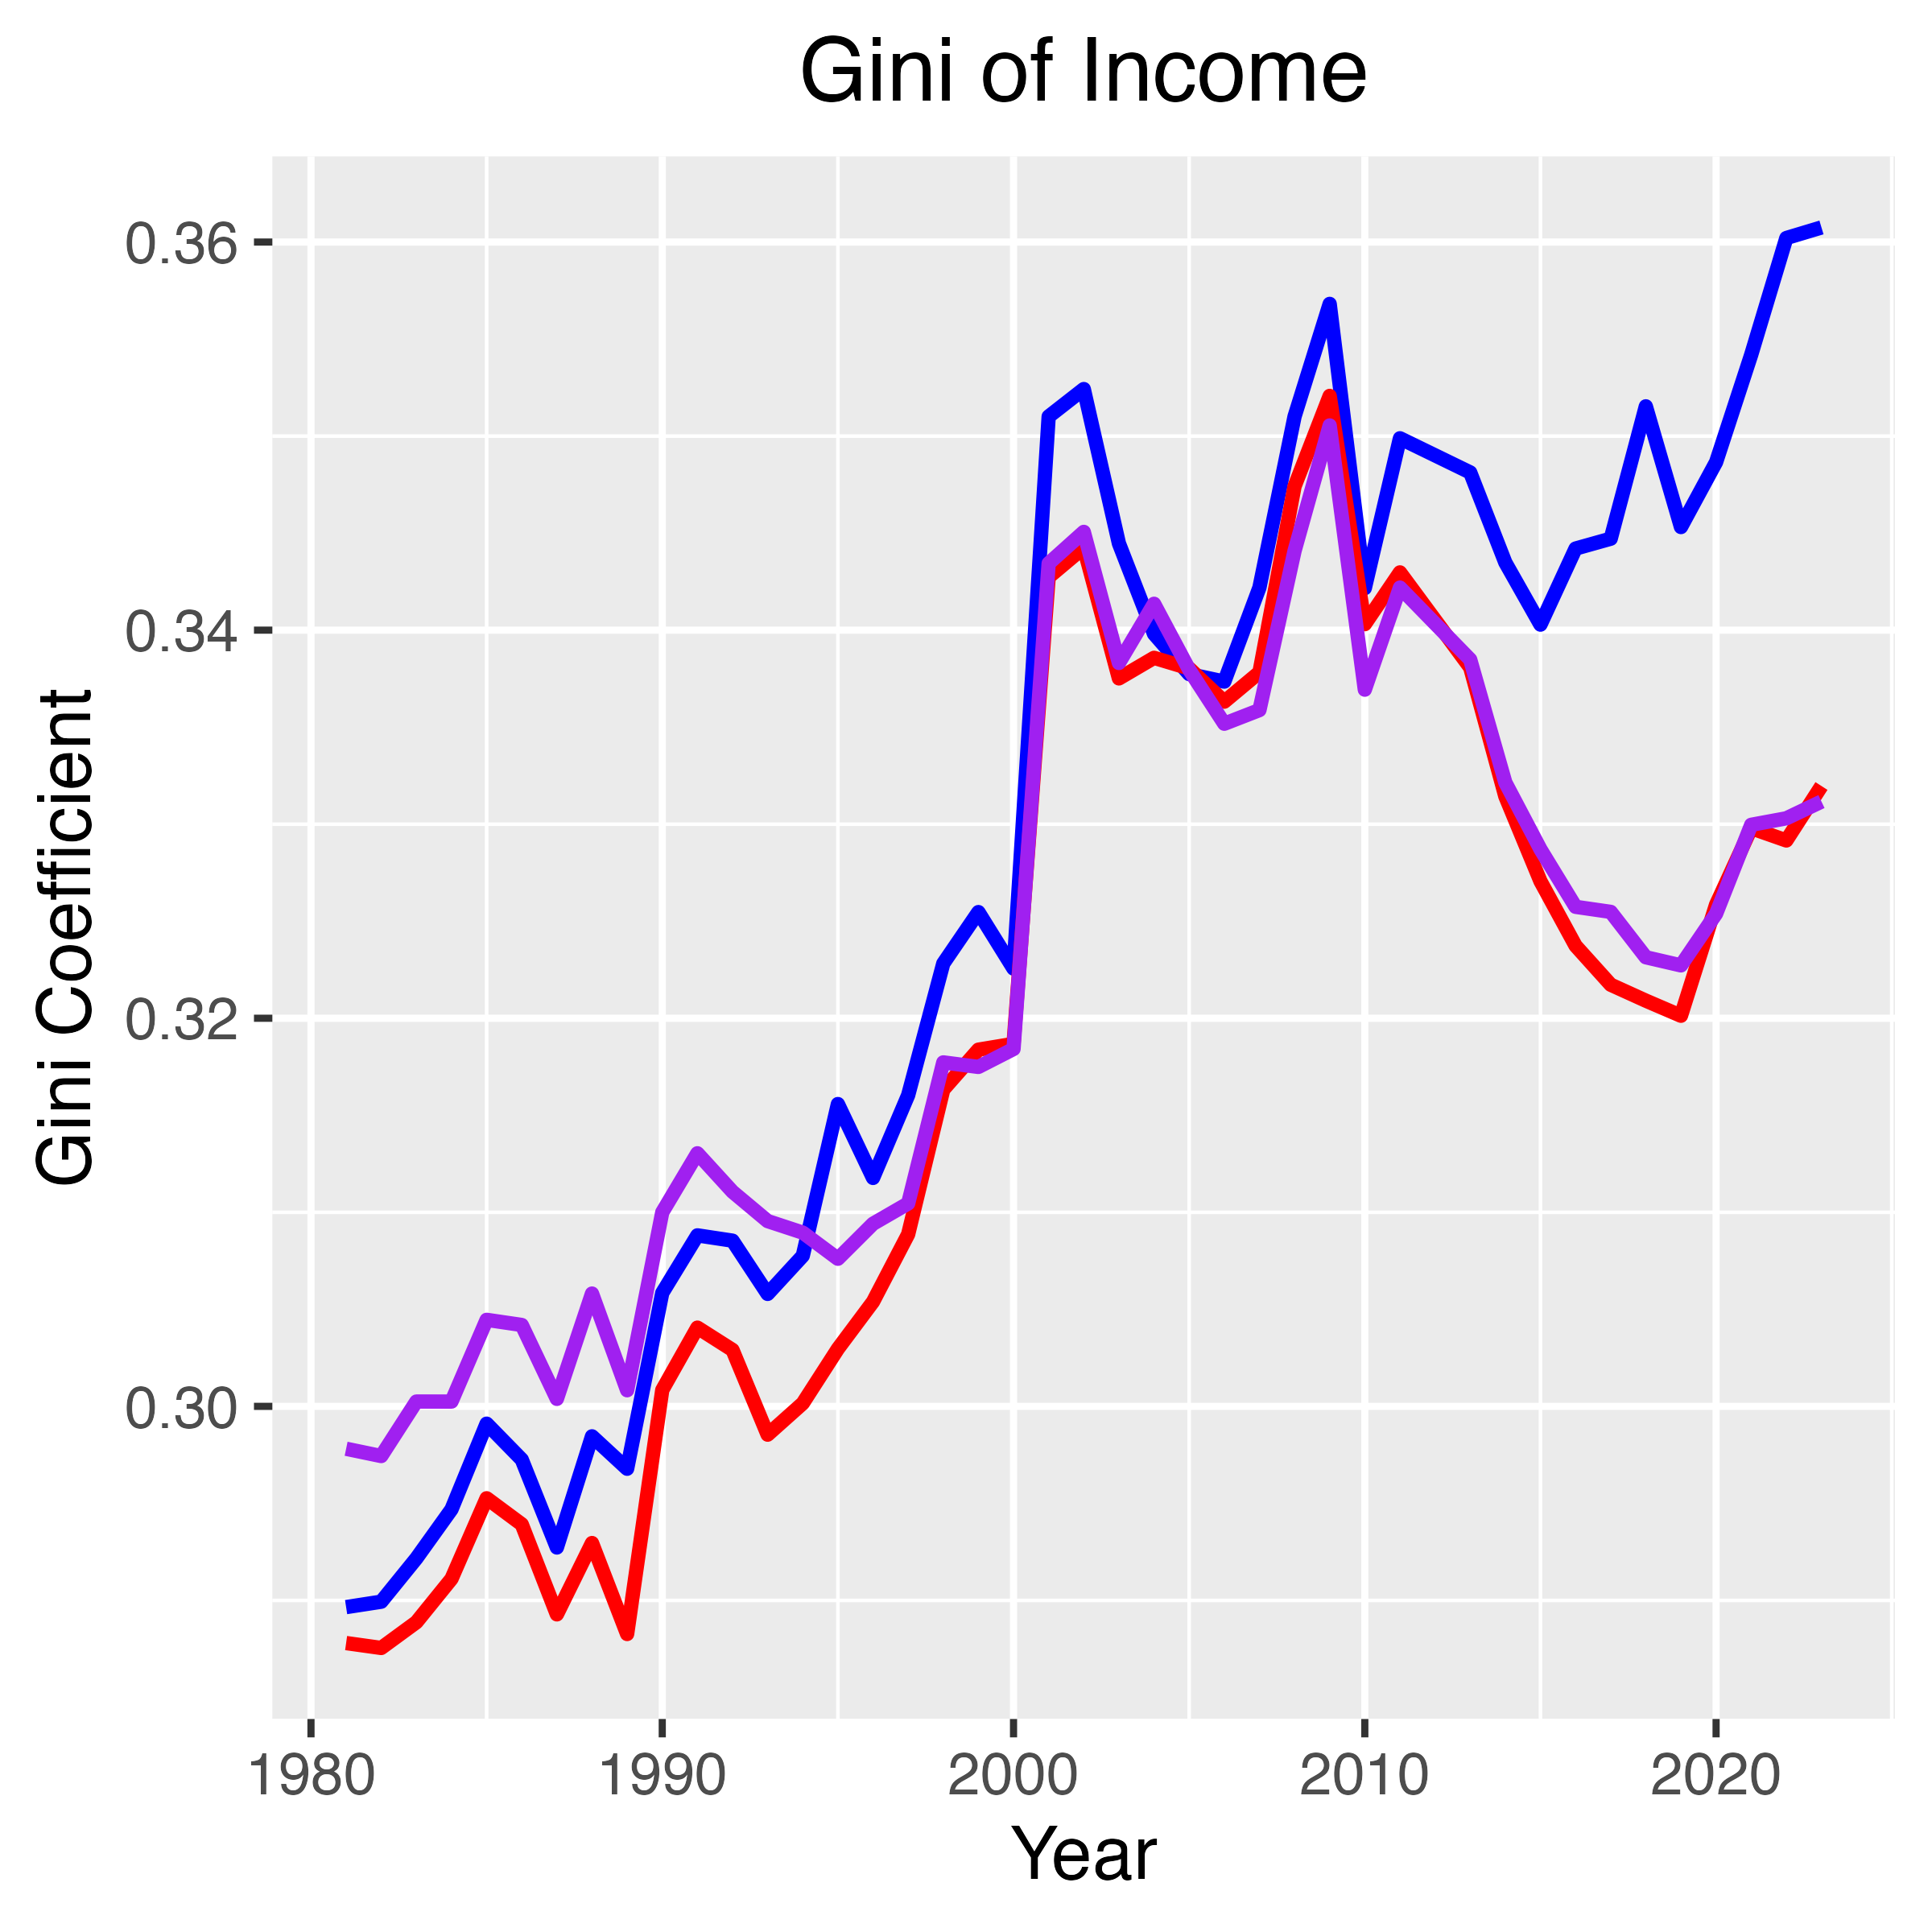
\includegraphics[width=\textwidth]{figures/Fig_4/Fig_4d_Gini_inc.png}
    \end{subfigure}
    \caption{From Household Earnings to Pre-Government Income}
    \label{fig:Trans_Asset}
\end{figure}

In Figure \ref{fig:Trans_Asset}, we discuss other income sources beyond basic earnings, including investment in assets and private transfers. 
We can see that asset income increases inequality while transfers reduce it, suggesting that there is a negative correlation between income and private transfers. 
This correlation aligns with the assumption that beyond the household, the family or clan can smooth out income shock using private transfer. 
In particular, the effect of private transfer smoothing out asset inequality was not effective before 1995. However, it has played a key role in reducing inequality since 2010.

\begin{figure}[t]
    \centering
    \begin{subfigure}[t]{0.475\textwidth}
        \centering
        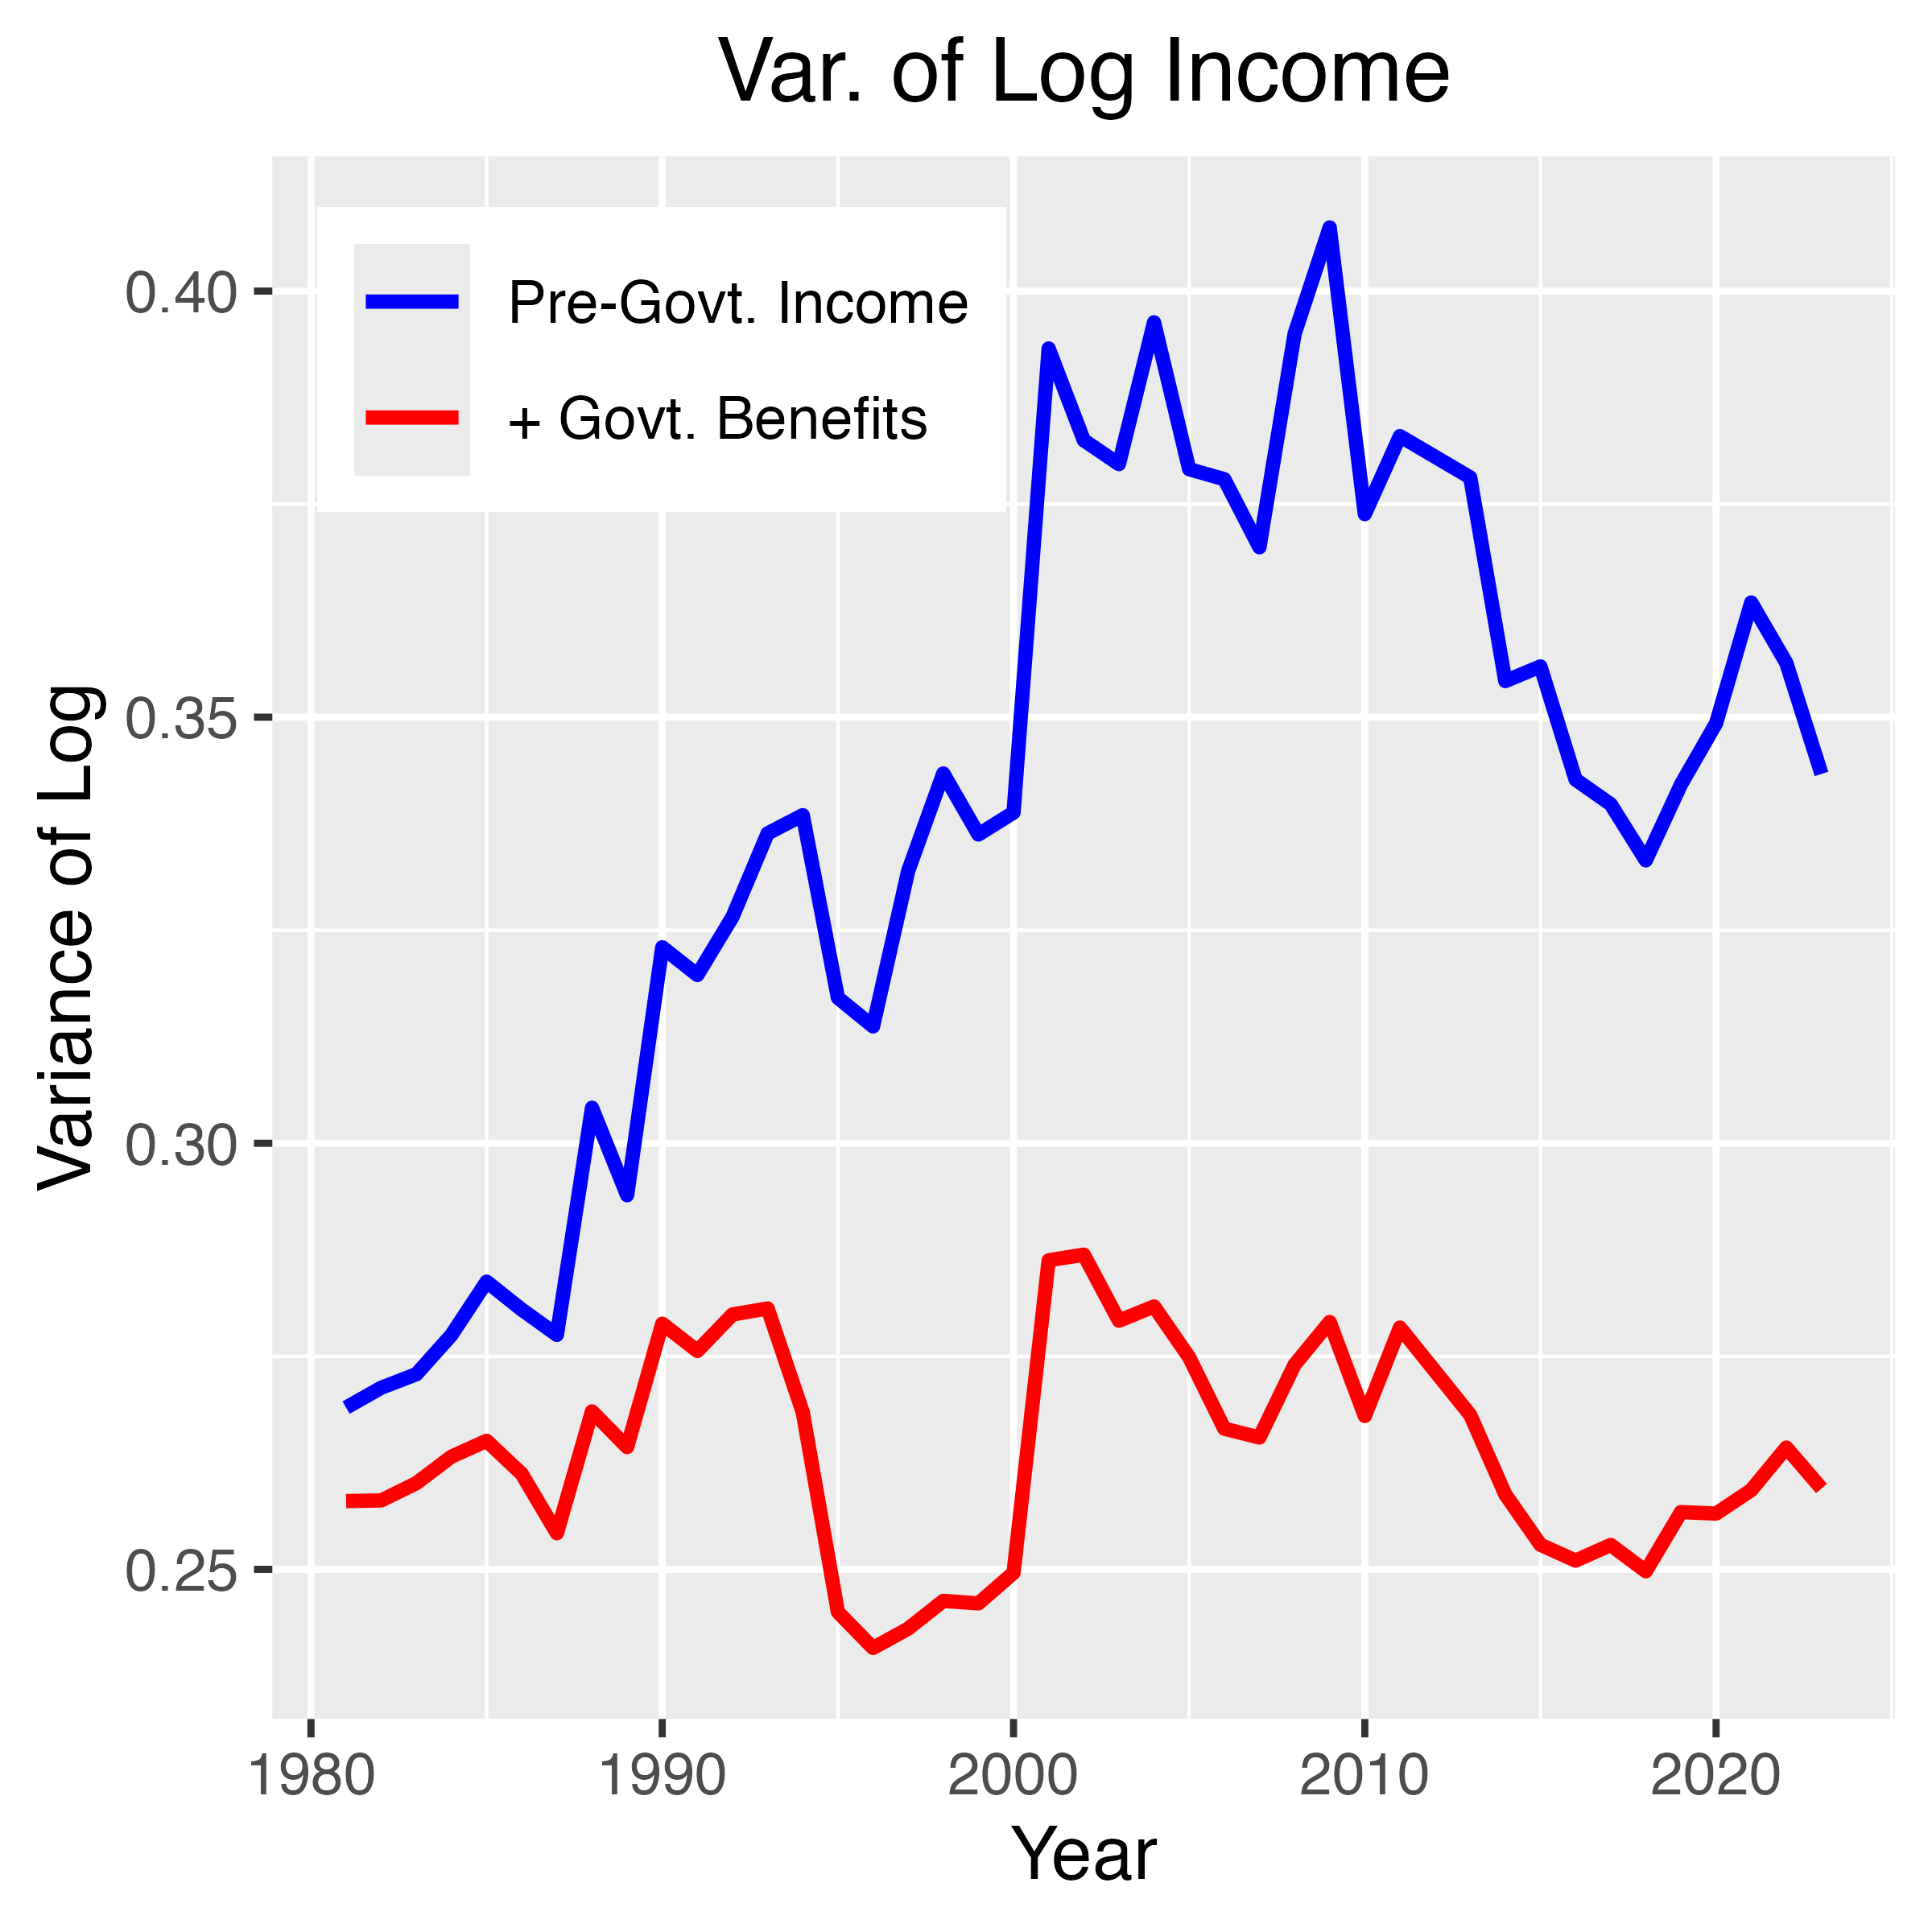
\includegraphics[width=\textwidth]{figures/Fig_5/Fig_5a_Var_inc.png}
    \end{subfigure}
    \begin{subfigure}[t]{0.475\textwidth}
        \centering
        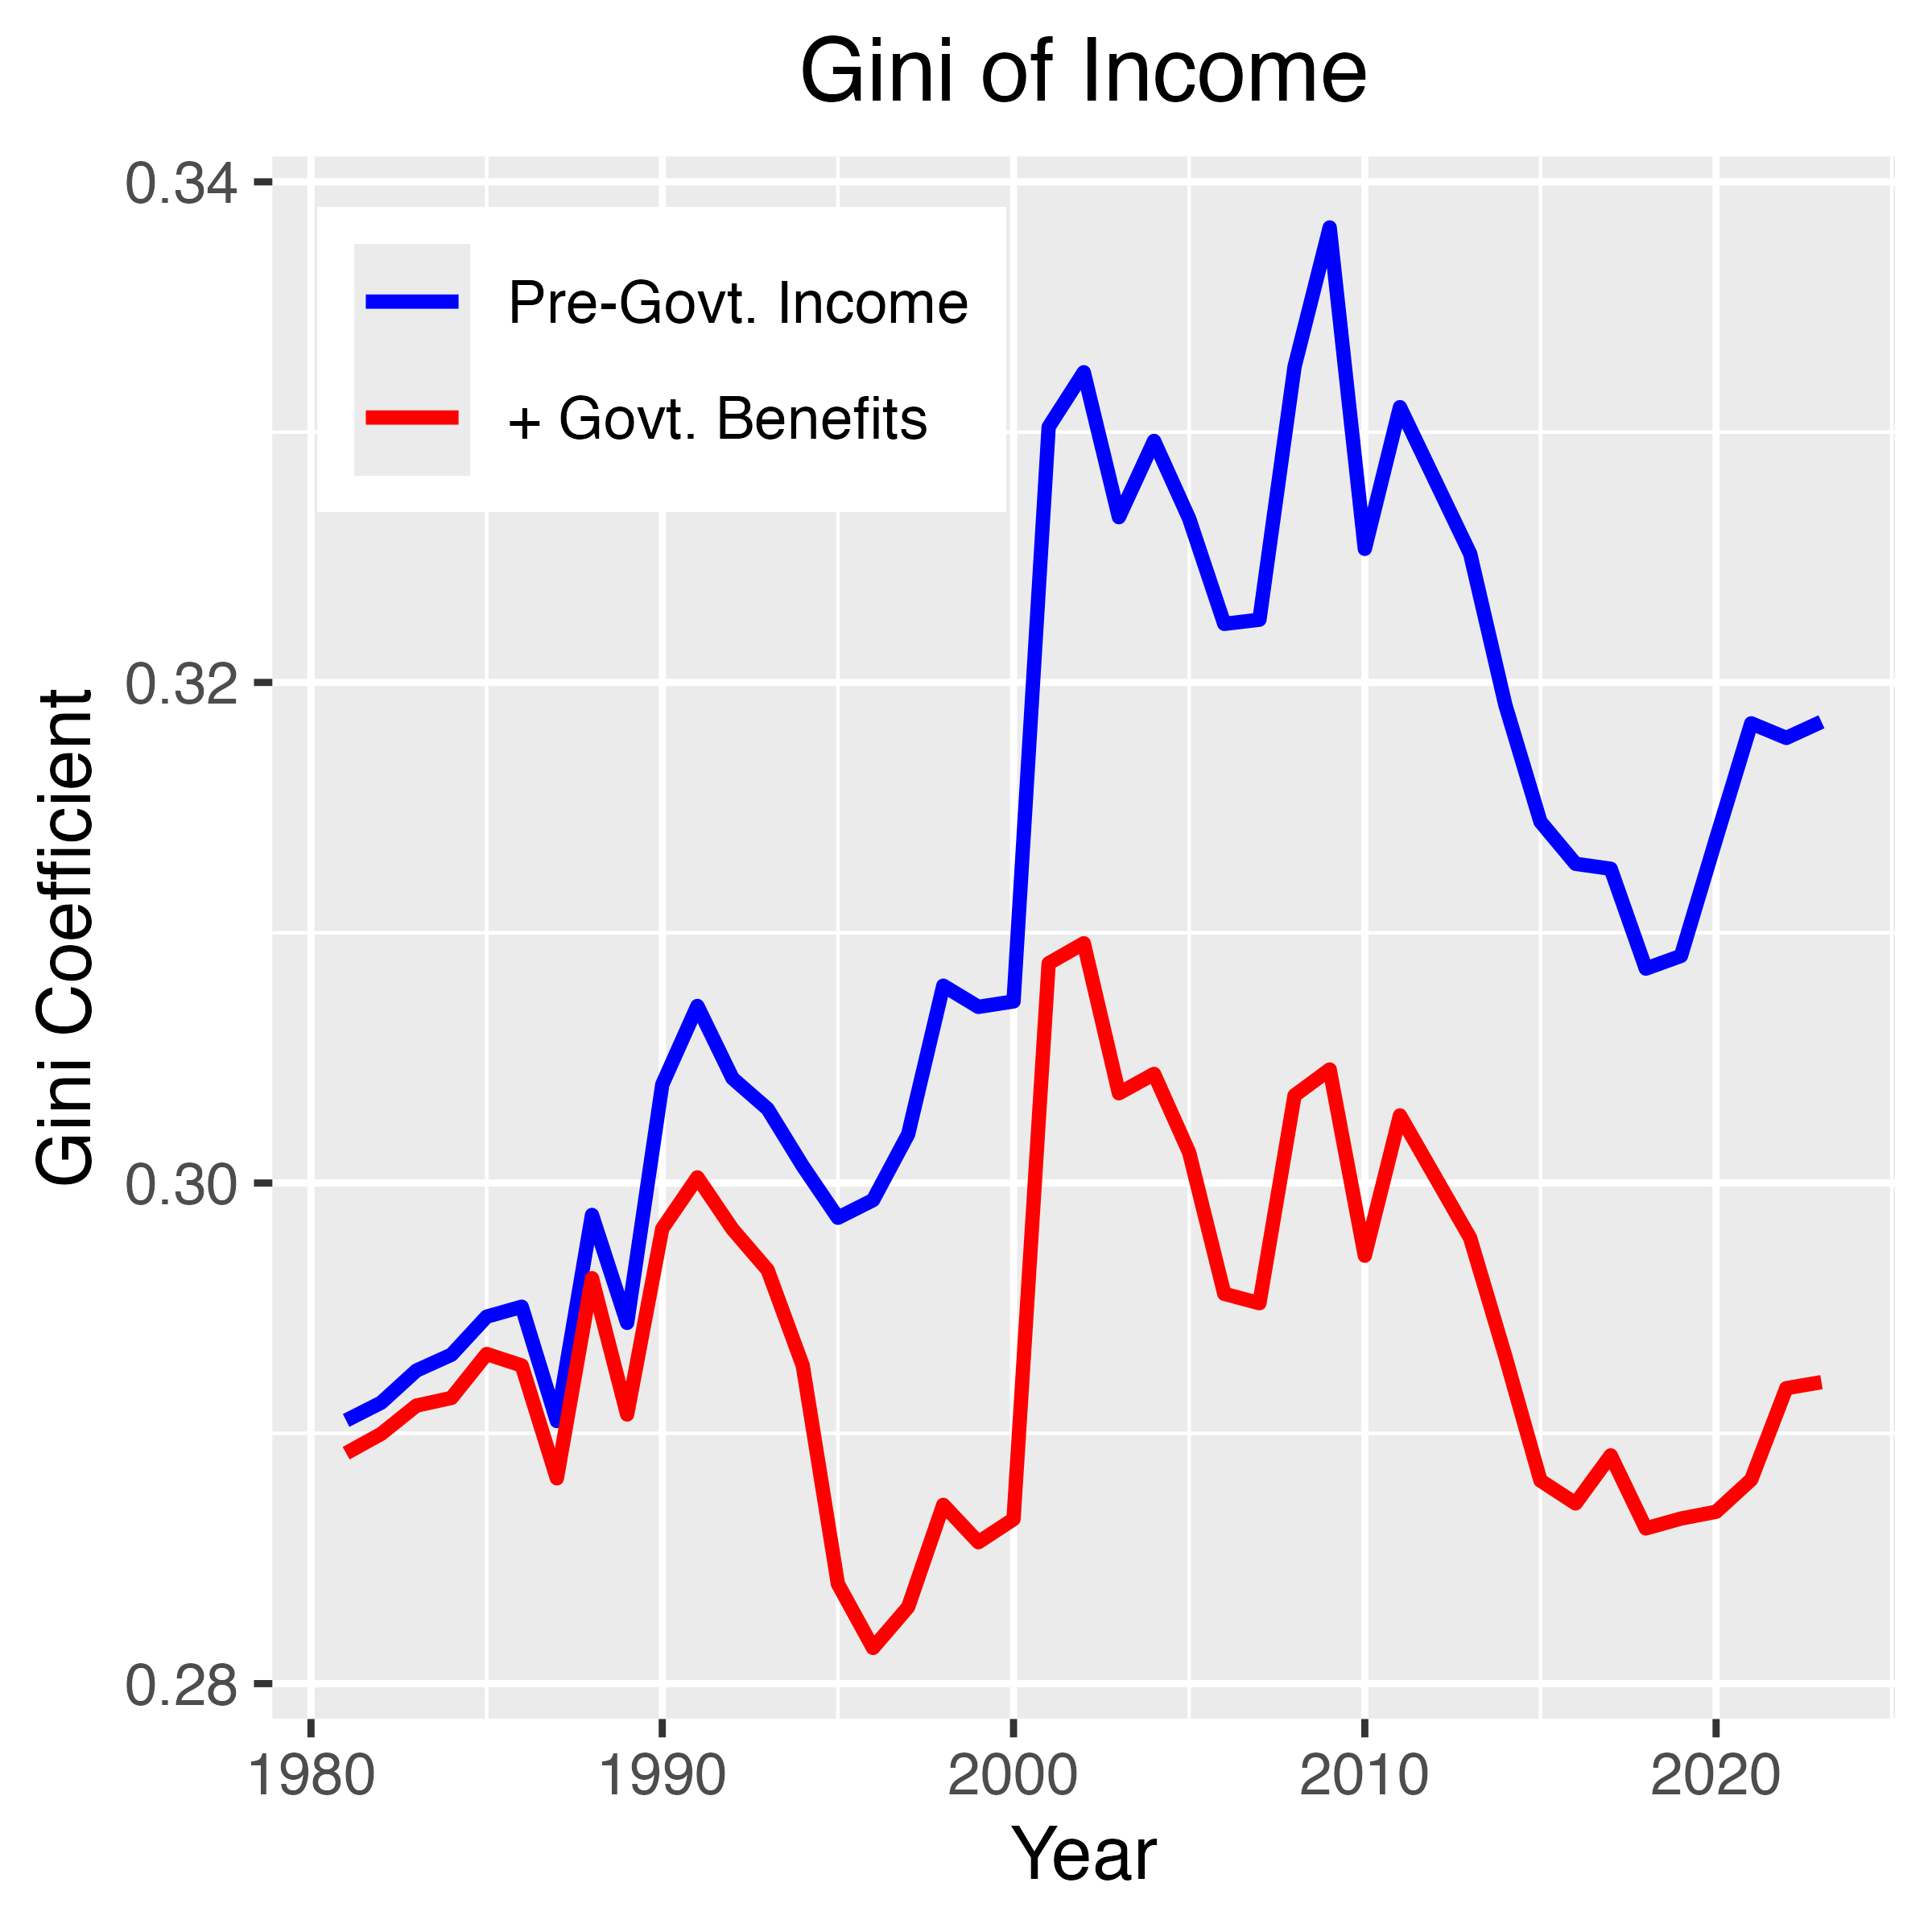
\includegraphics[width=\textwidth]{figures/Fig_5/Fig_5b_Gini_inc.png}
    \end{subfigure}
    \begin{subfigure}[t]{0.475\textwidth}
        \centering
        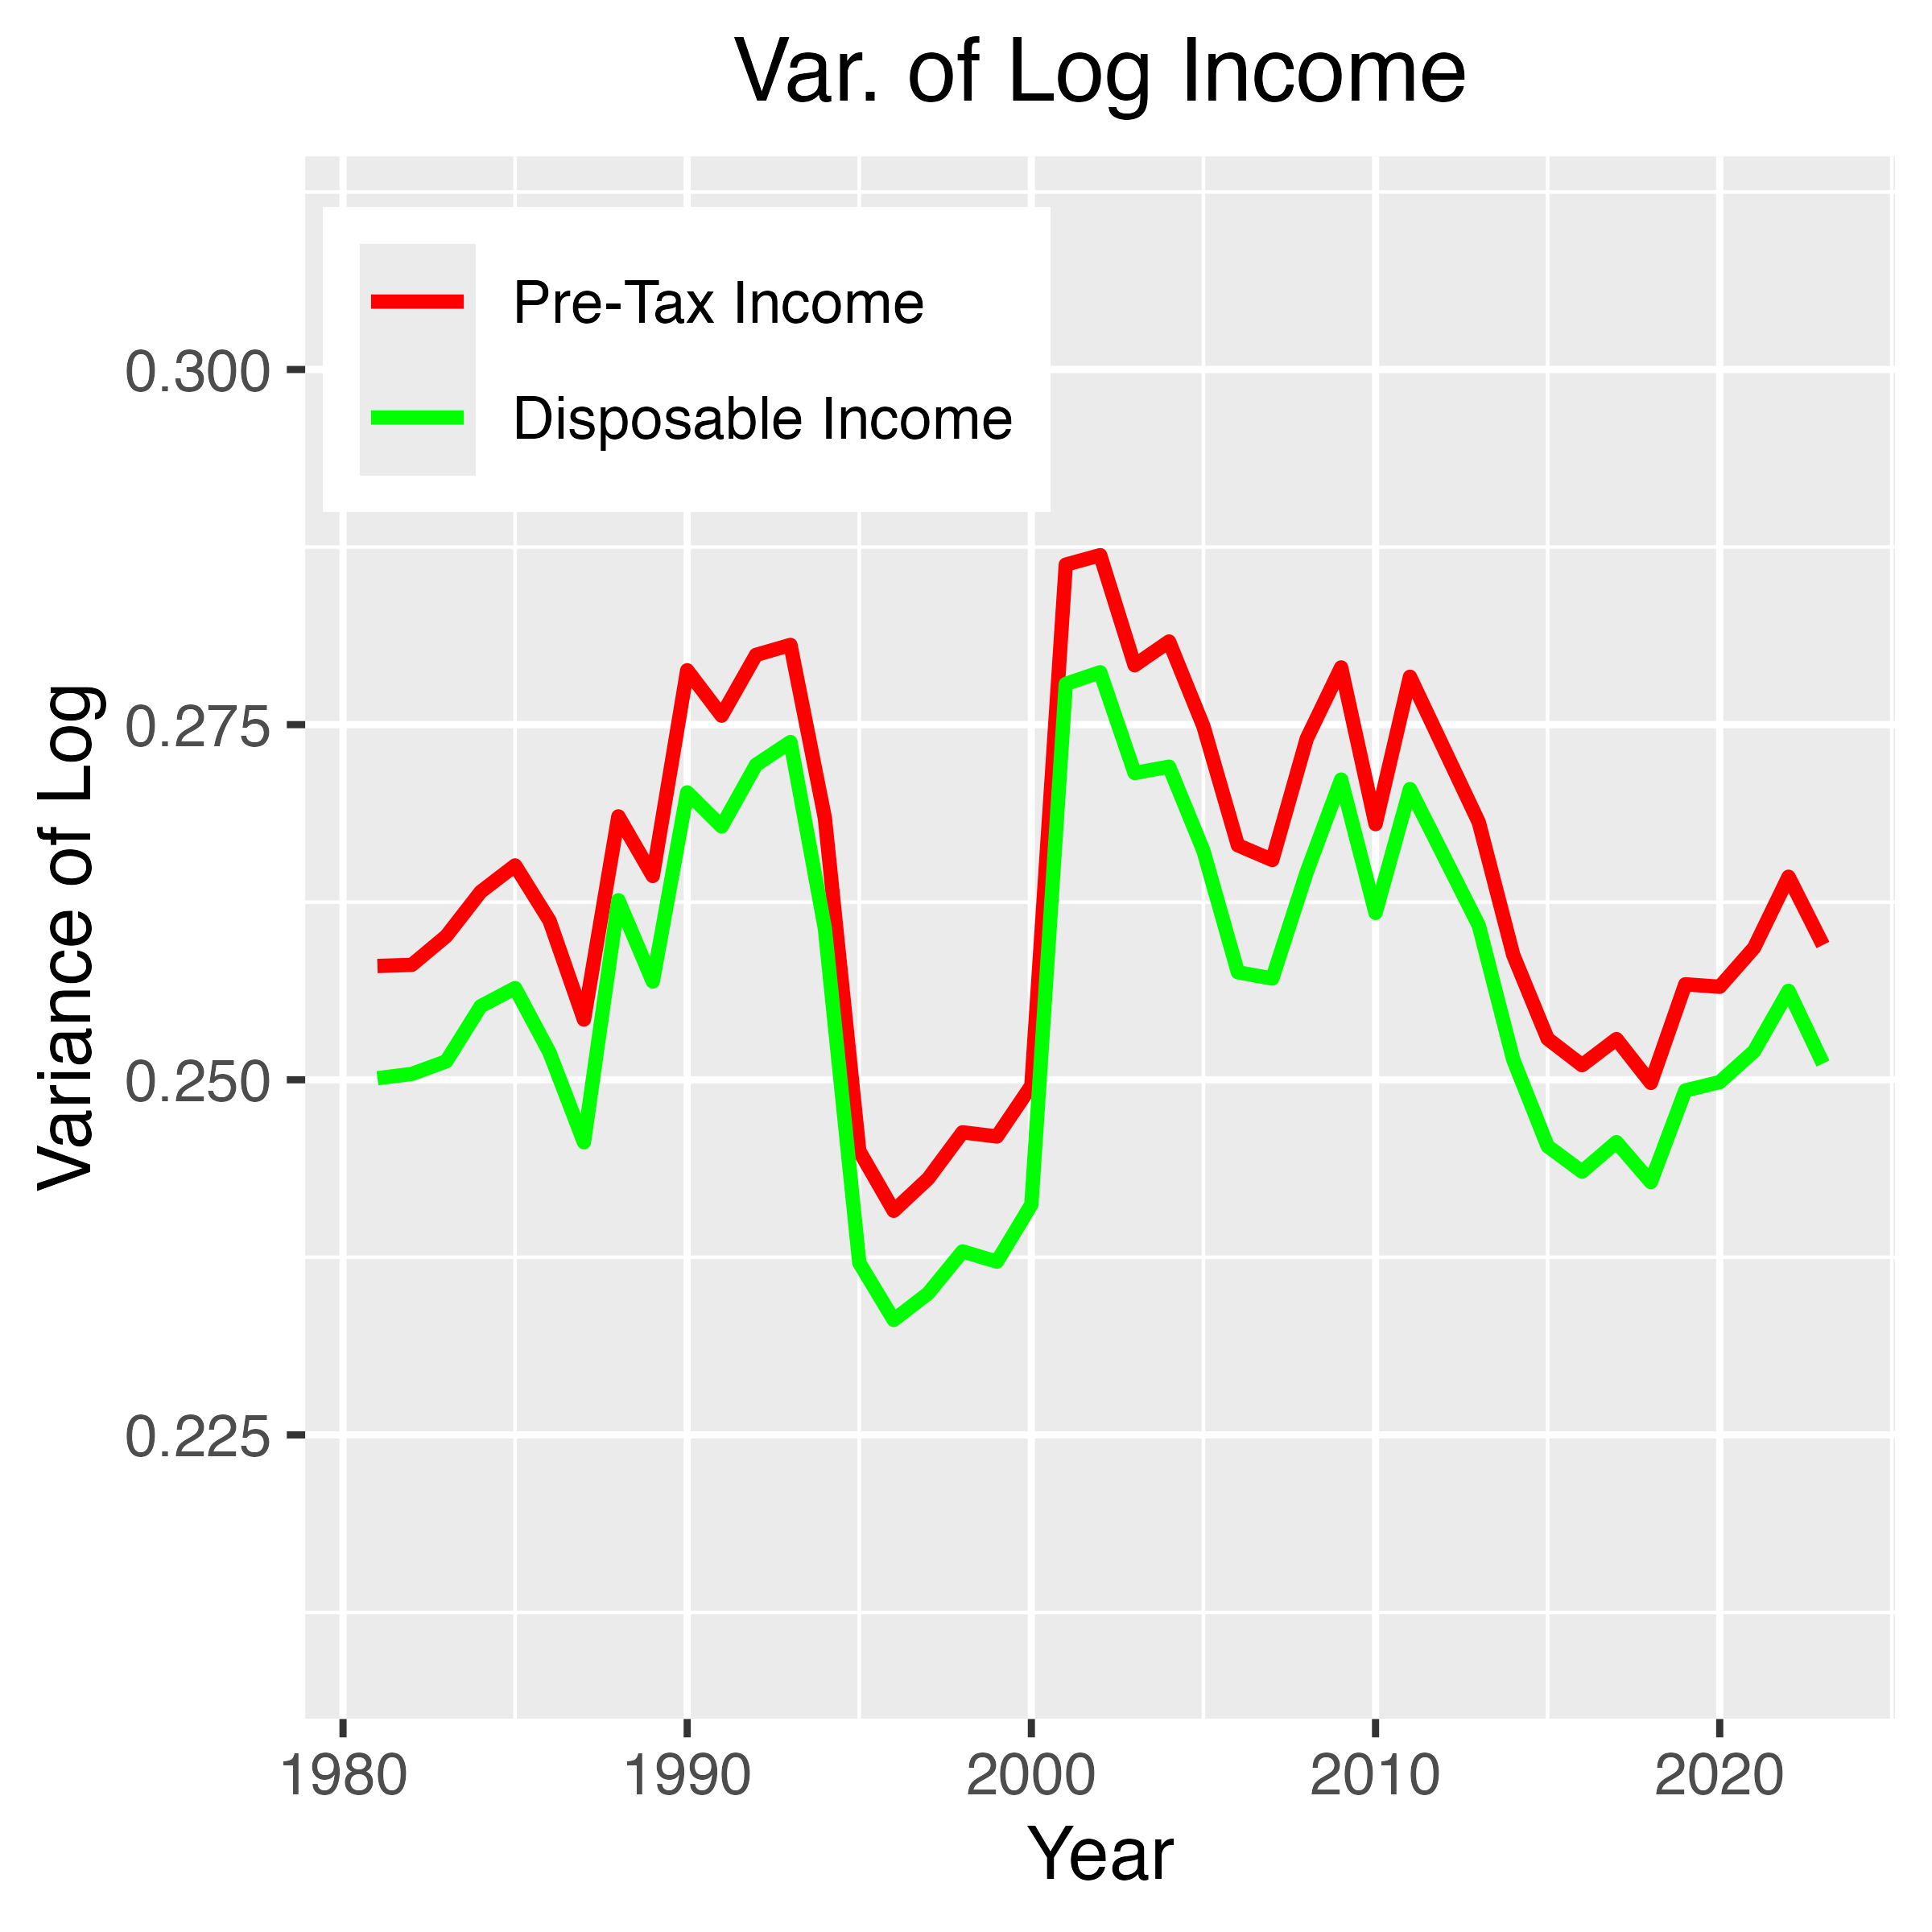
\includegraphics[width=\textwidth]{figures/Fig_5/Fig_5c_Var_inc.png}
    \end{subfigure}
    \begin{subfigure}[t]{0.475\textwidth}
        \centering
        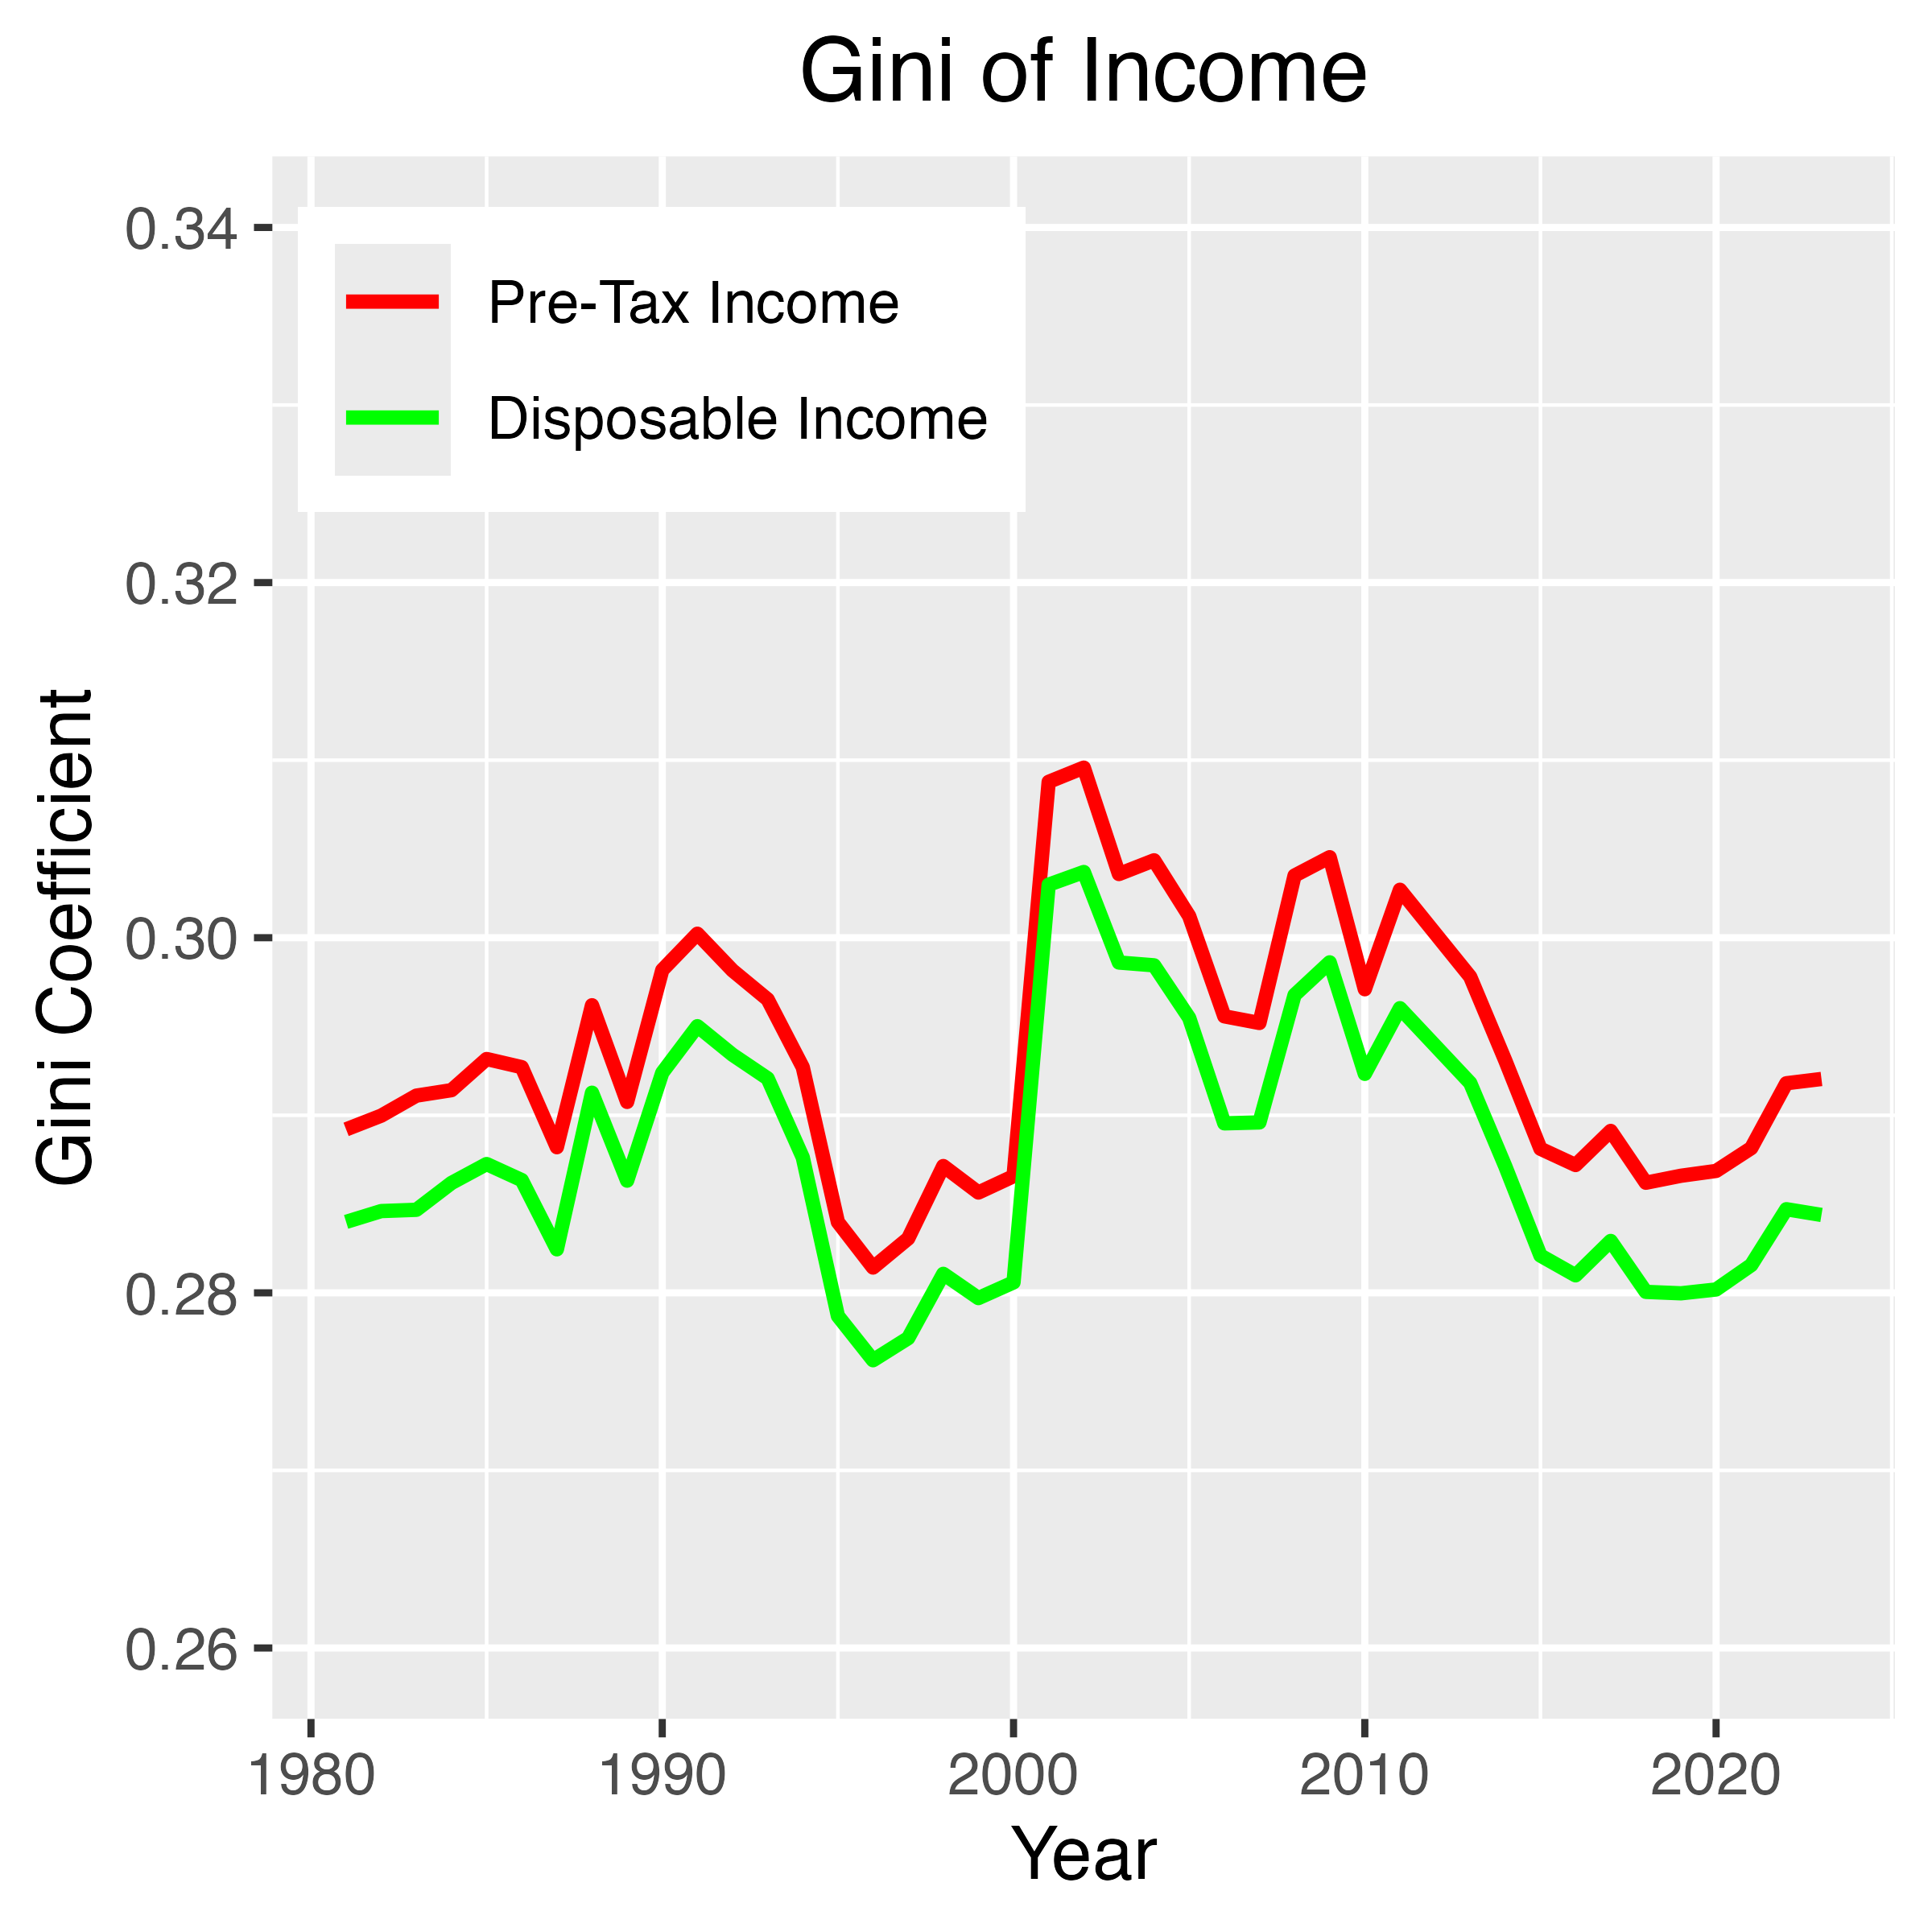
\includegraphics[width=\textwidth]{figures/Fig_5/Fig_5d_Gini_inc.png}
    \end{subfigure}
    \caption{From Pre-Government to Disposable Income}
    \label{fig:Gov}
\end{figure}

\subsection{Government Redistribution}

We move on to government redistribution in Figure \ref{fig:Gov}. Redistribution plays a significant role in reducing income inequality. We can see that although both subsidy and taxation measures reduce inequality, welfare systems such as public health insurance and labor insurance have a more substantial redistribution effect. The benefits reduce the Gini coefficient for about 3 log points, and tax further reduces it by 0.5 log points, resulting in a much smoother trend.

Compared to the increased variance and Gini coefficient of Pre-Government income, redistribution successfully stabilized the income inequality, making the Gini coefficient stable around 0.3. However, the government did not smooth out the drastic increase of inequalities during recessions like the Dot-com bubble in 2000 and the Global Financial Crisis in 2008. Surprisingly, COVID-19 after 2020 did not increase inequalities significantly; this can be due to the government's subsidy and expenditure, which successfully stabilized the disparity at the time.

\subsection{From Income to Consumption Inequality}

The rest of this section discusses consumptions and expenditures. Figure \ref{fig:Consumption} shows the exact four measurements of Figure \ref{fig:earnings_inequality} for disposable income and consumption; the result highlights the effect of consumption smoothing. Since households can borrow and save to maintain consumption when facing income shock, consumption inequality is smaller than income.

Surprisingly, compared to the US, where consumption inequality increased, consumption discrepancies in Taiwan decreased steadily after 1995. One of the reasons could be the low consumption growth rate of wealthy families, as shown in figure \ref{fig:Consumption_cyclic}. The consumption expenditures of the top 5\% families only grow about 12 log points compared to 36 log points in the lowest 25 \%. 

These consumption phenomena could negatively impact Taiwan's economy, suggested by Hong (\citeyear{TW_stable_dist}), since wealthy families do not increase their consumption and lower-income families face higher housing and health insurance burdens. Eventually, this led to a stagnation of Taiwan's economy.

\begin{figure}[p]
    \centering
    \begin{subfigure}[t]{0.475\textwidth}
        \centering
        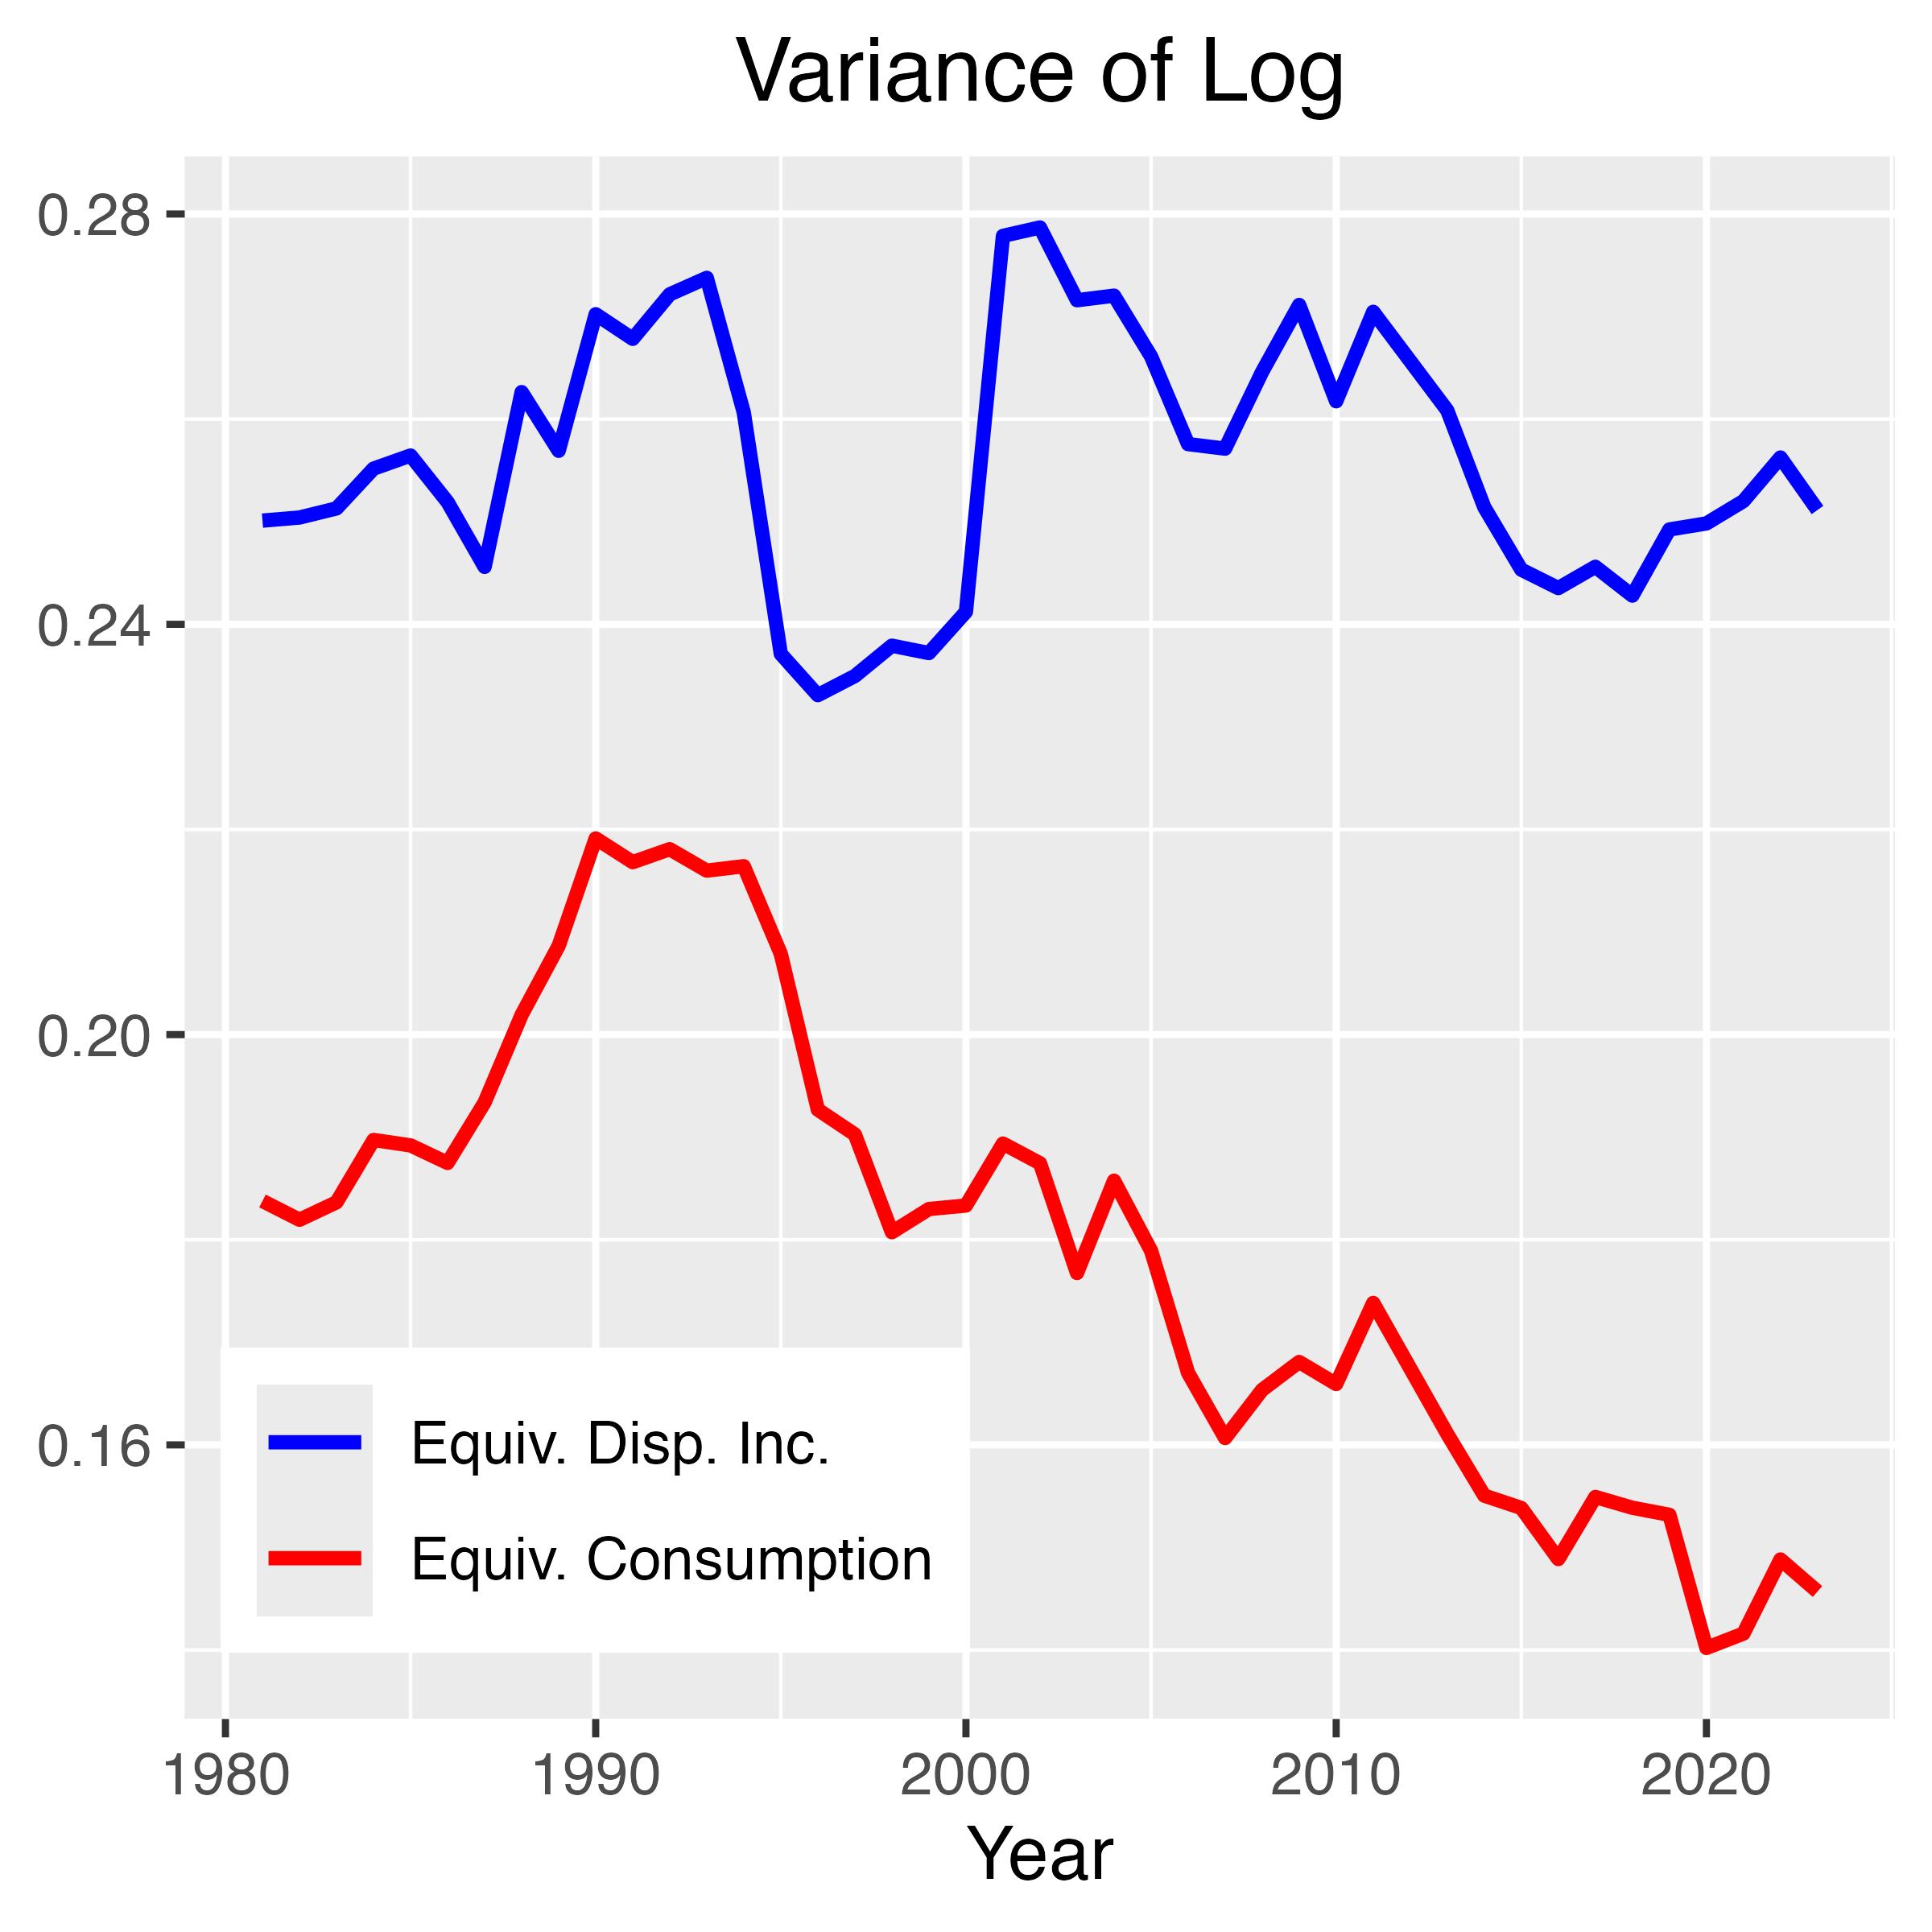
\includegraphics[width=\textwidth]{figures/Fig_6/Fig_6a.png}
    \end{subfigure}
    \begin{subfigure}[t]{0.475\textwidth}
        \centering
        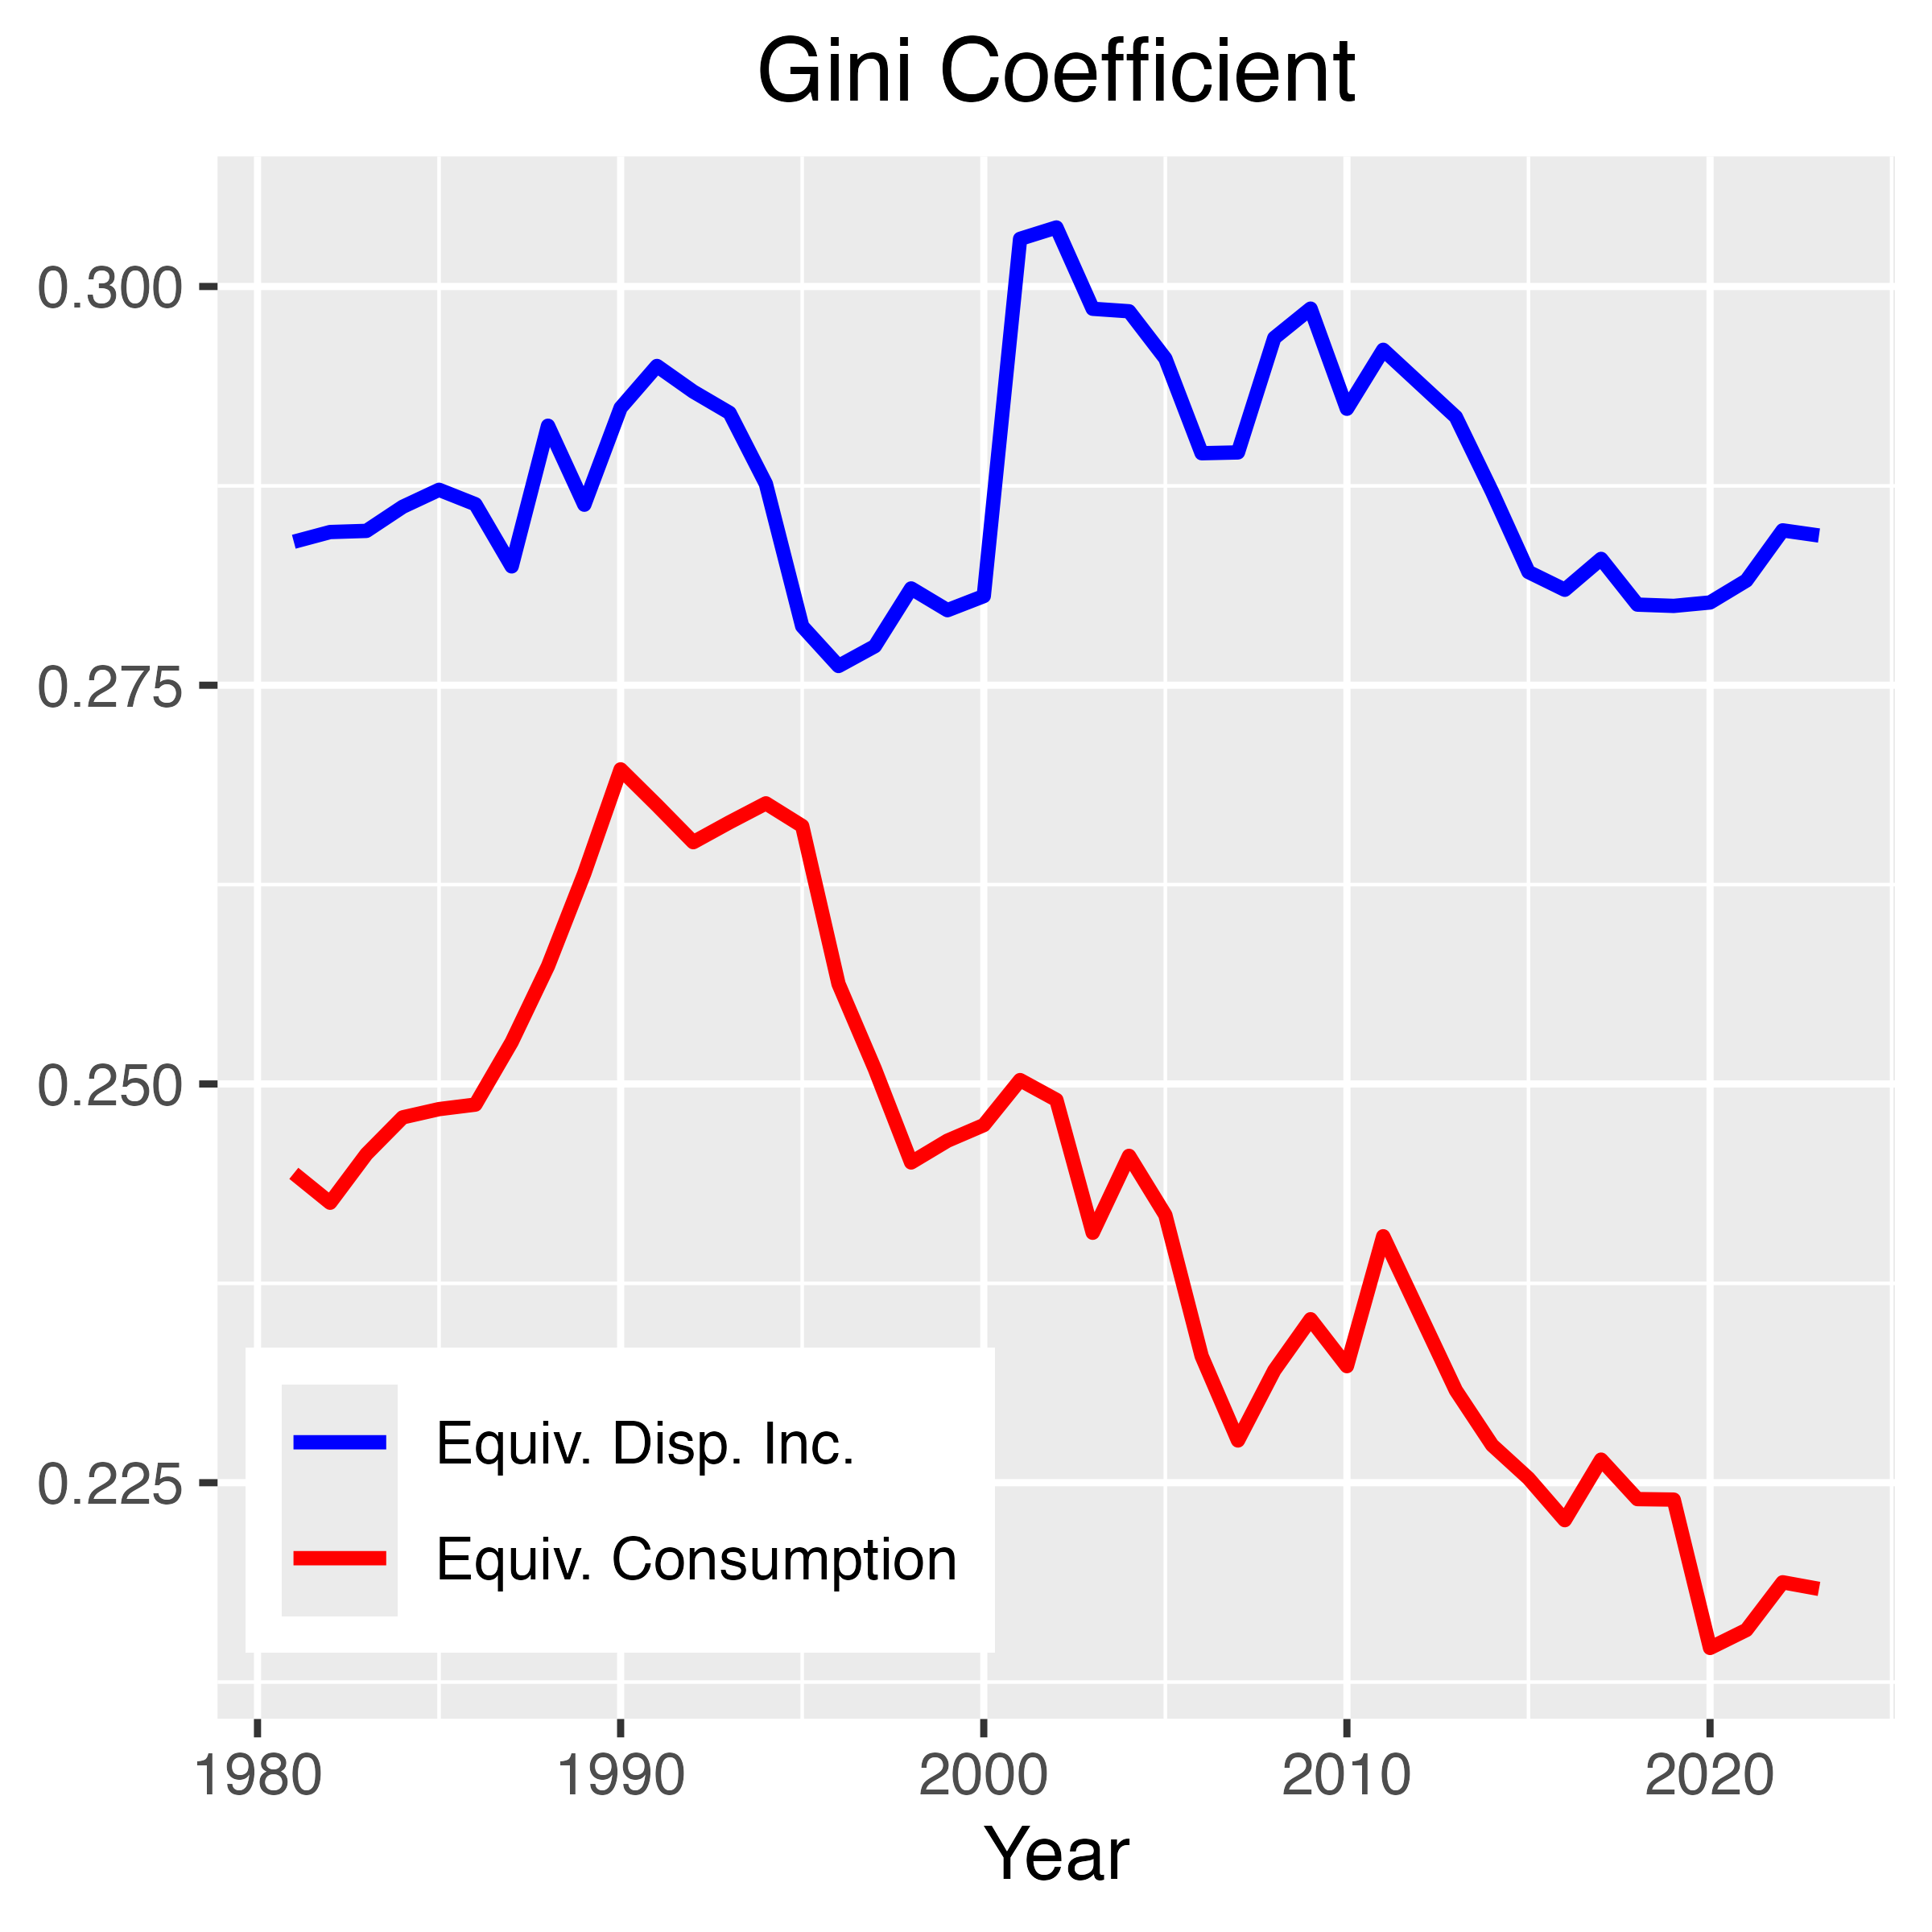
\includegraphics[width=\textwidth]{figures/Fig_6/Fig_6b.png}
    \end{subfigure}
    \begin{subfigure}[t]{0.475\textwidth}
        \centering
        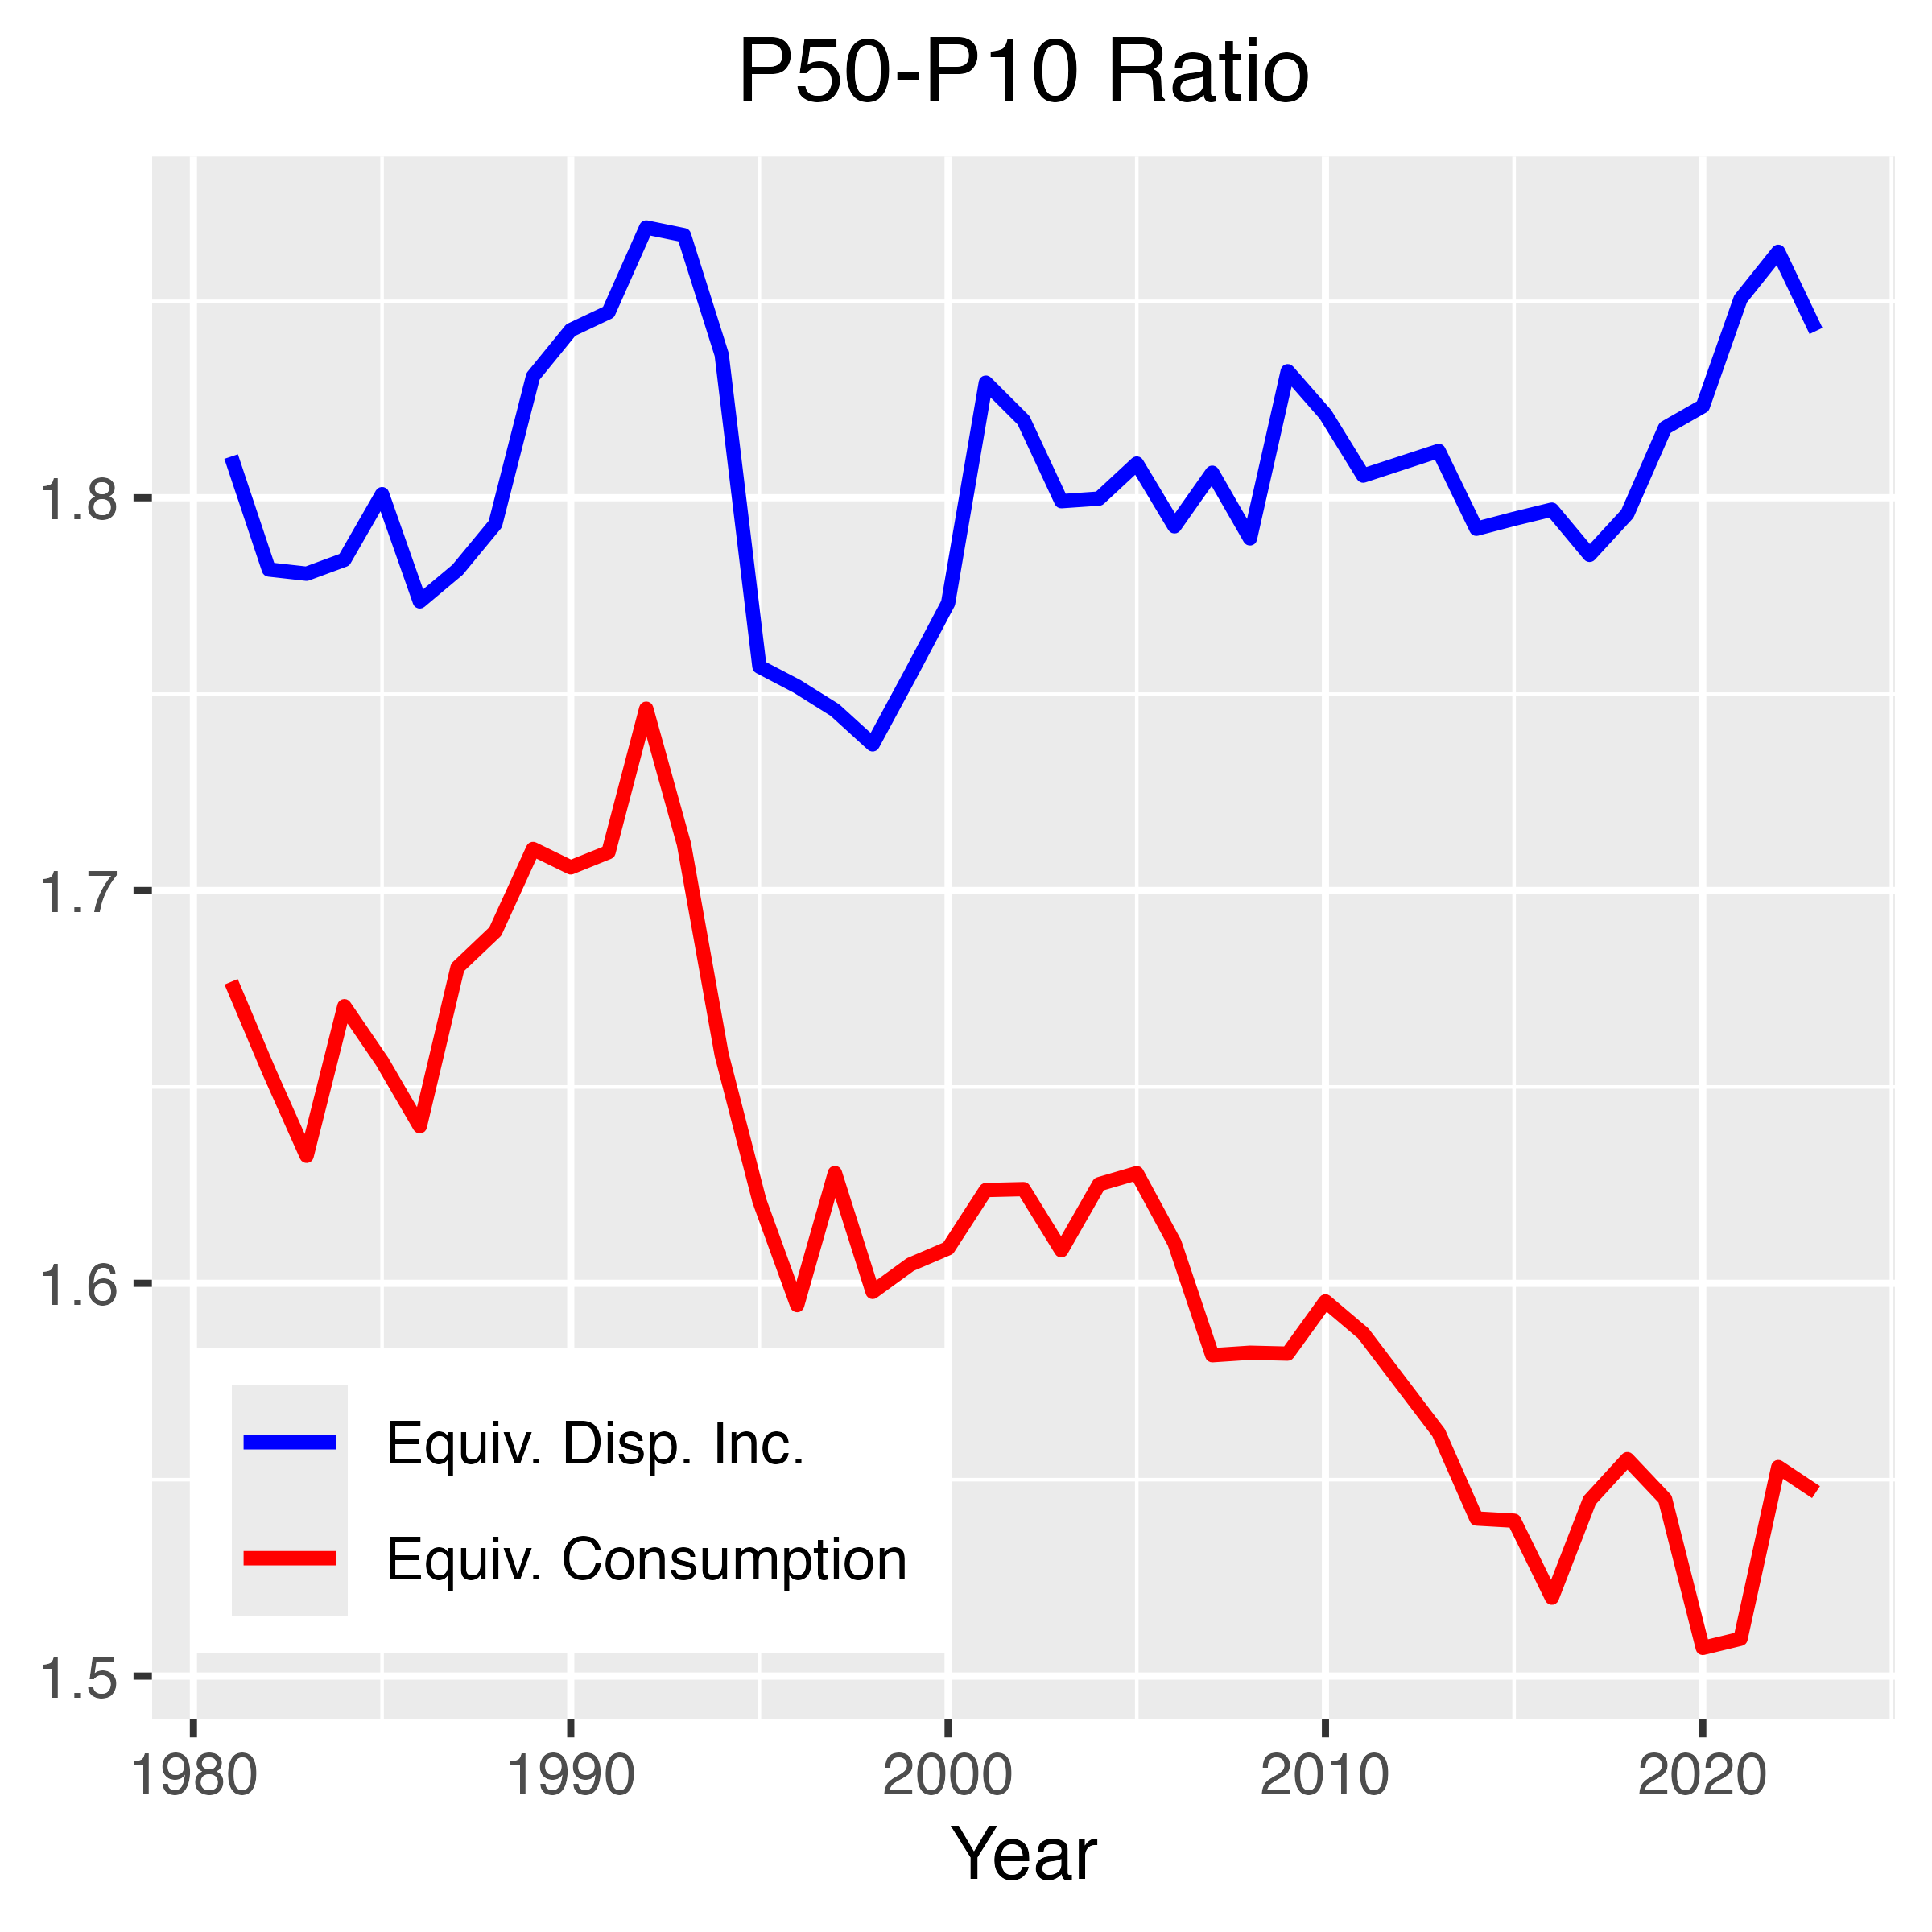
\includegraphics[width=\textwidth]{figures/Fig_6/Fig_6c.png}
    \end{subfigure}
    \begin{subfigure}[t]{0.475\textwidth}
        \centering
        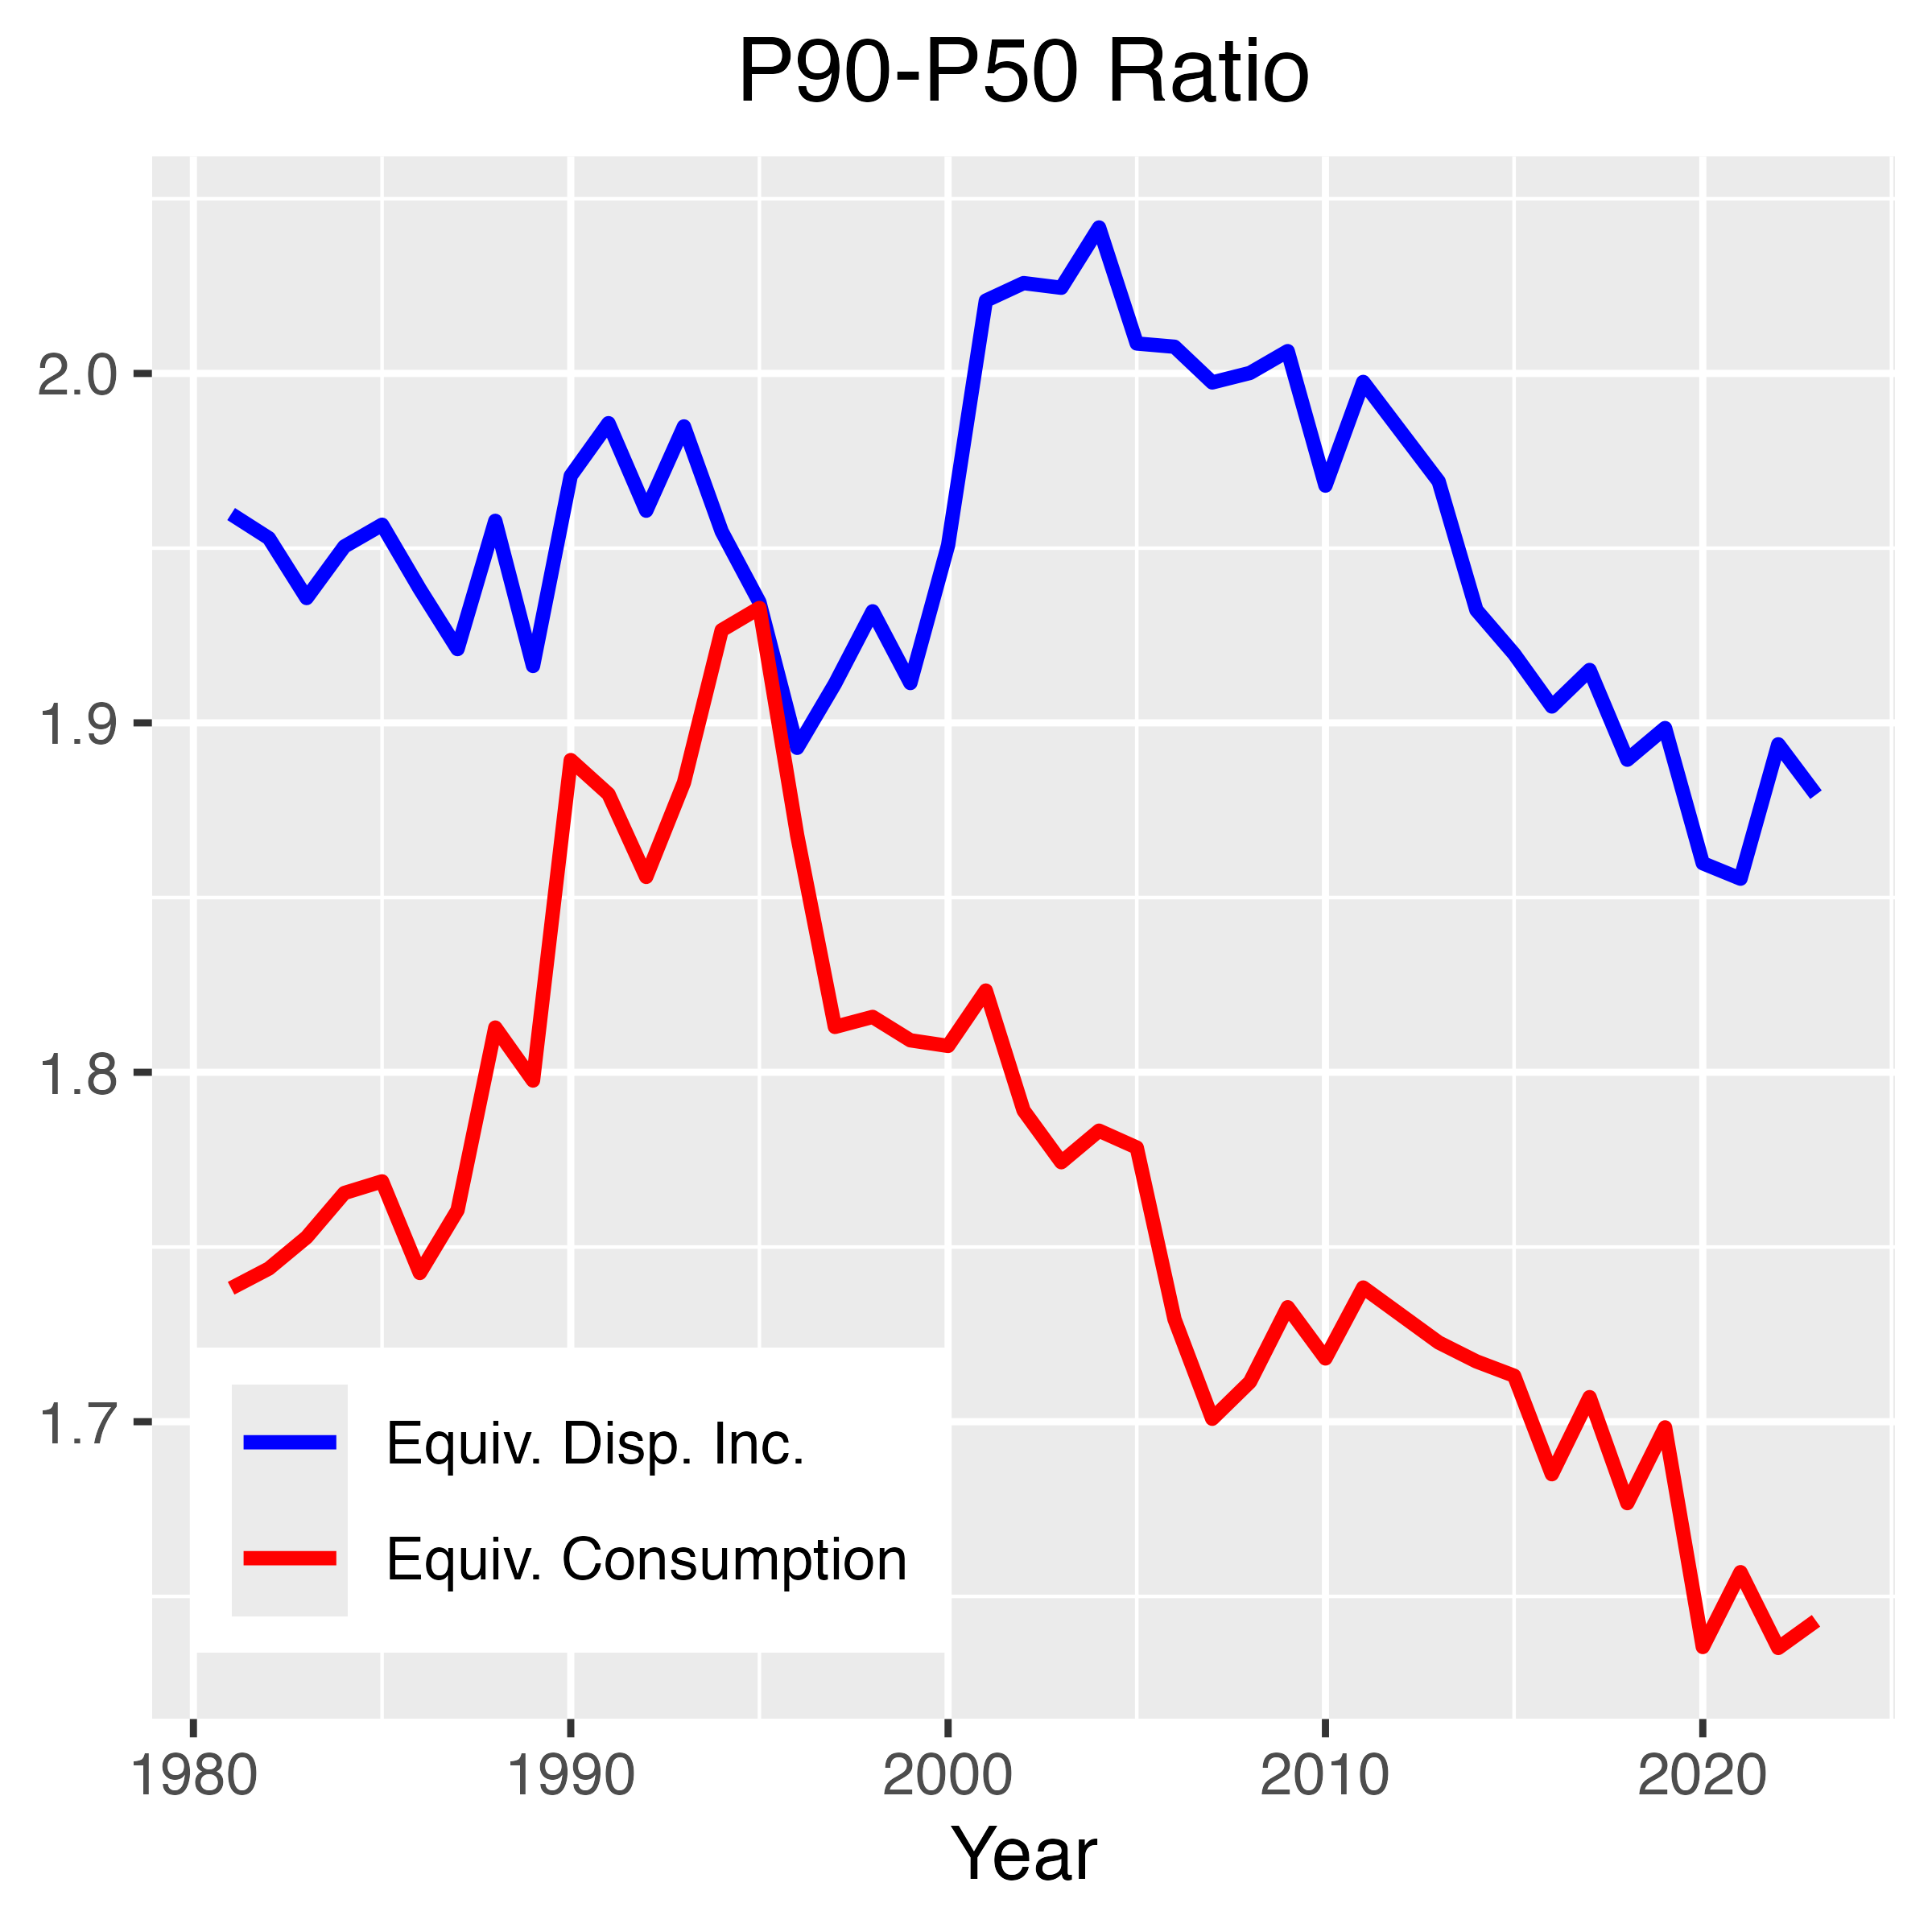
\includegraphics[width=\textwidth]{figures/Fig_6/Fig_6d.png}
    \end{subfigure}
    \caption{From Disposable Income to Consumption}
    \label{fig:Consumption}
    \vspace{1em}
    \centering
    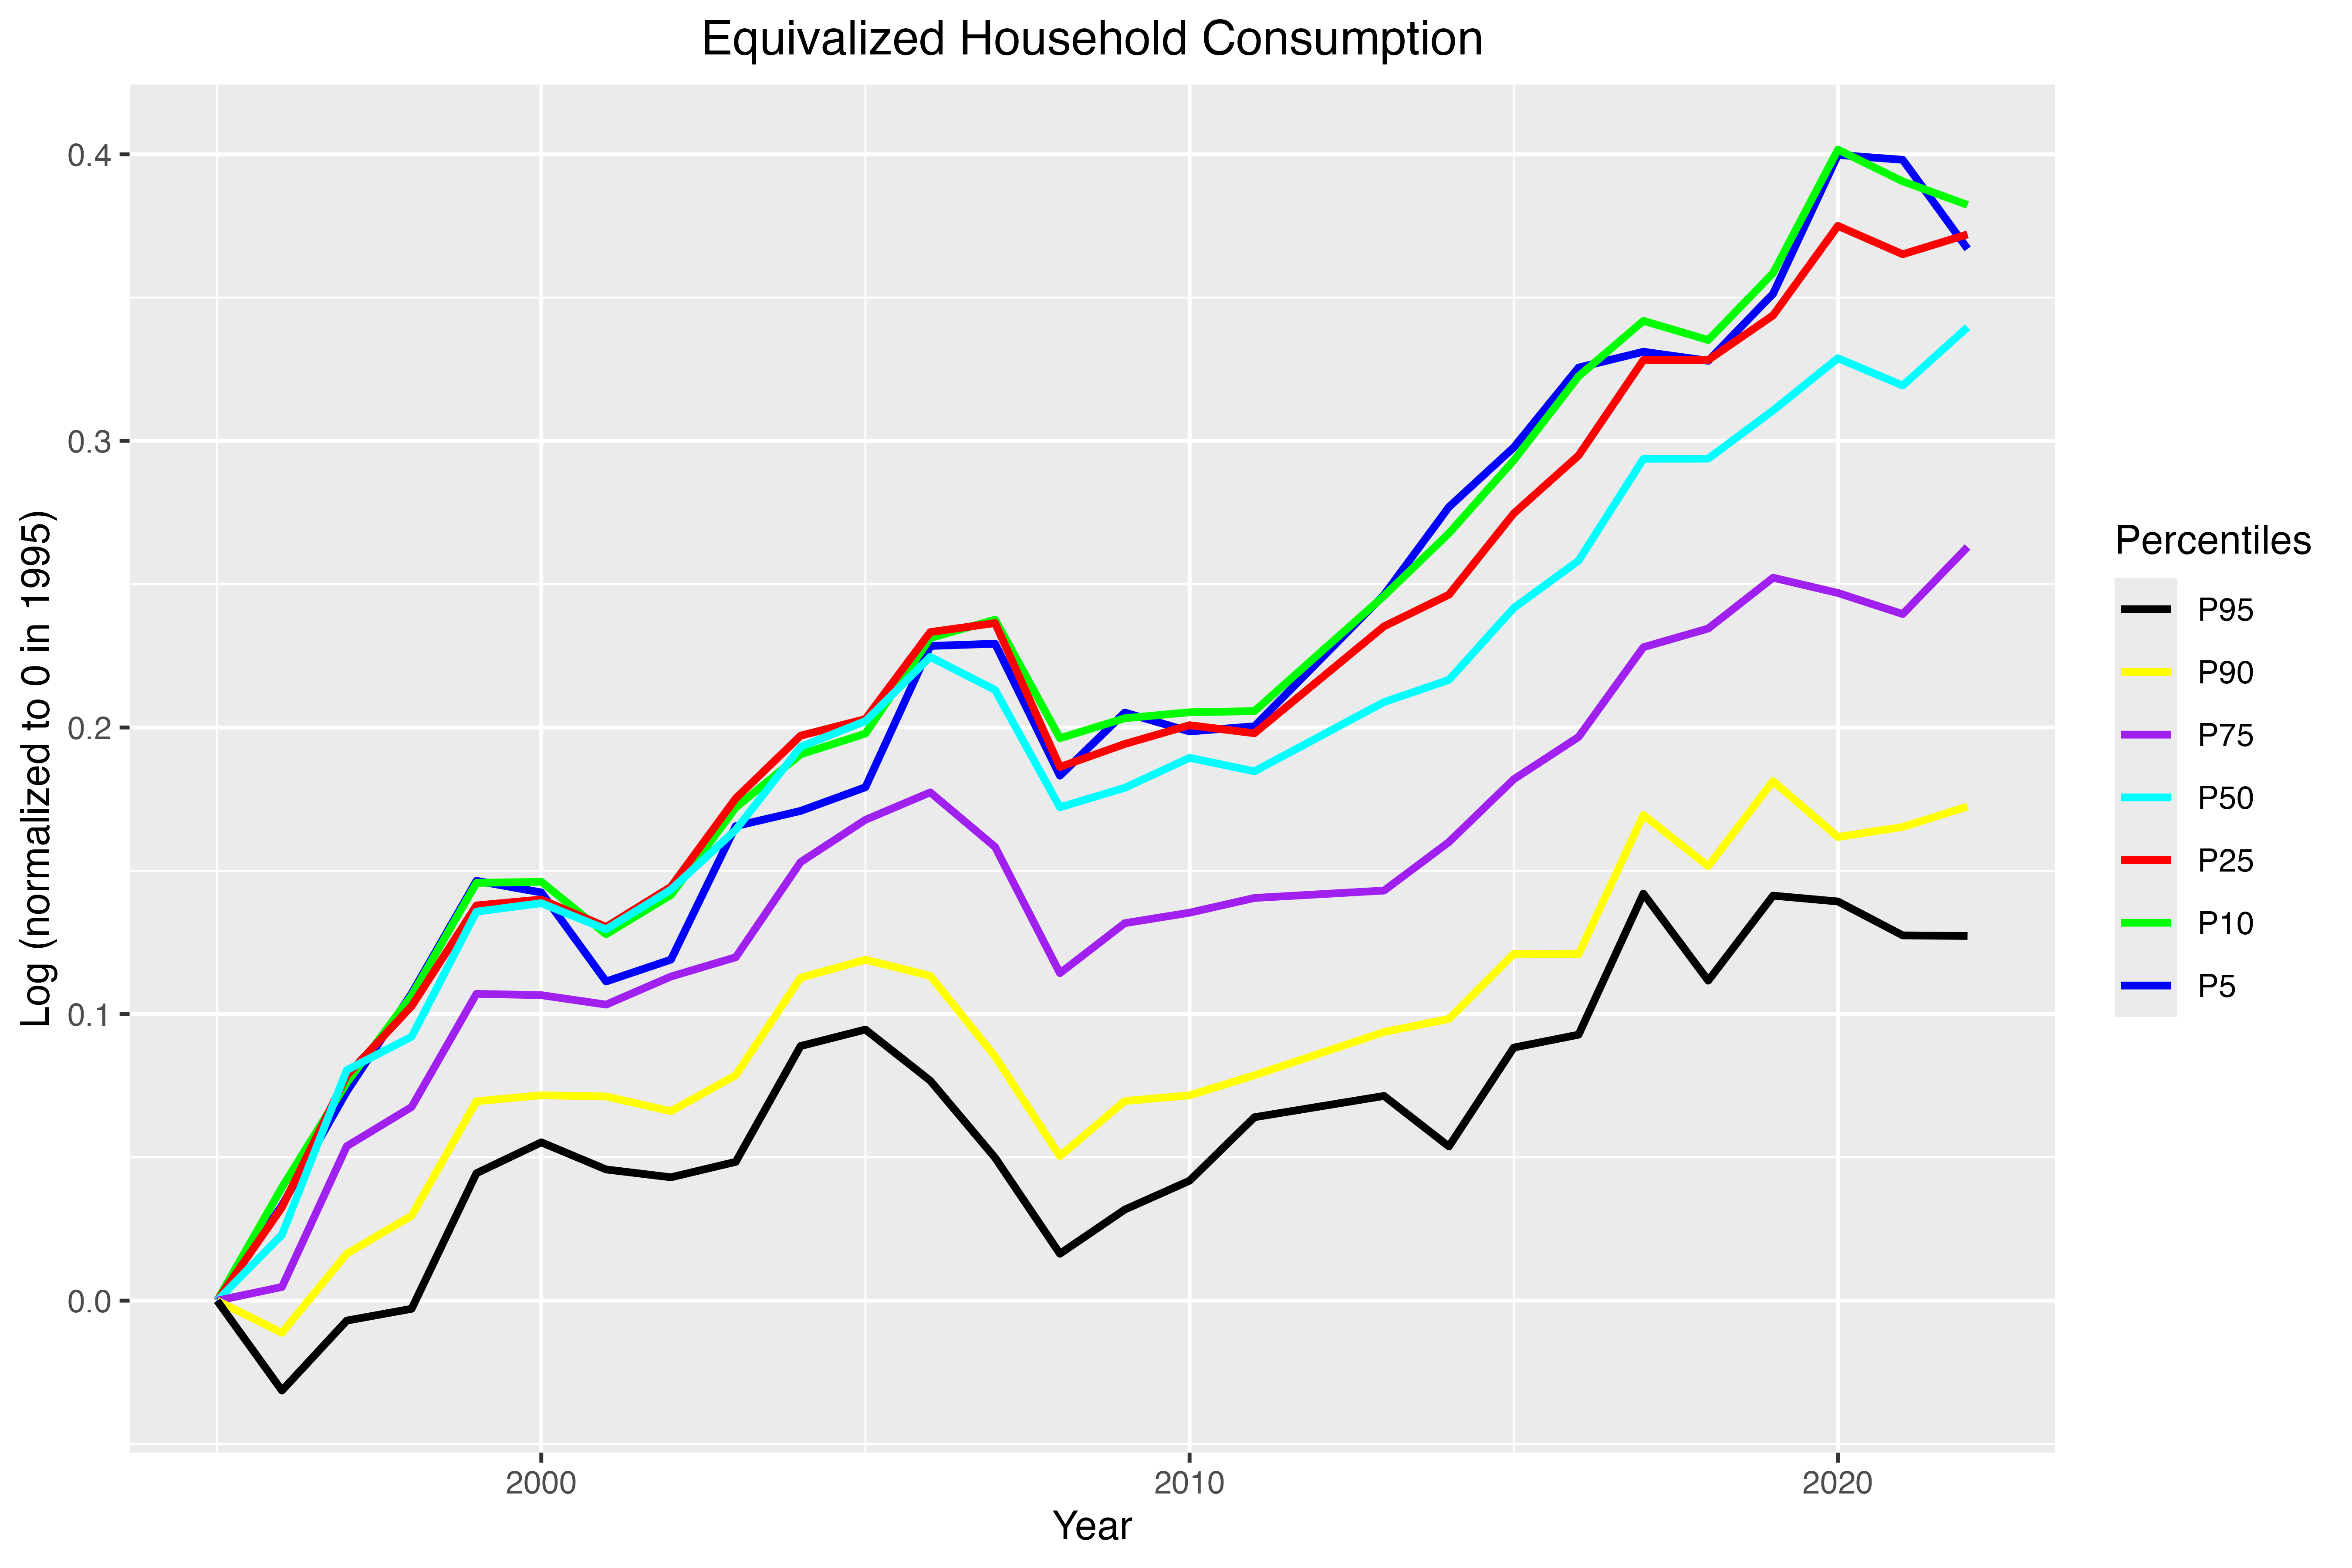
\includegraphics[width=0.95\textwidth]{figures/Fig_7/Fig_7_percentiles_a1995.png}
    \caption{Percentiles of the Household Consumption Distribution}
    \label{fig:Consumption_cyclic}
\end{figure}

\subsection{Food Consumption and Housing Services}

\begin{figure}
    \centering
    \begin{subfigure}[t]{0.475\textwidth}
        \centering
        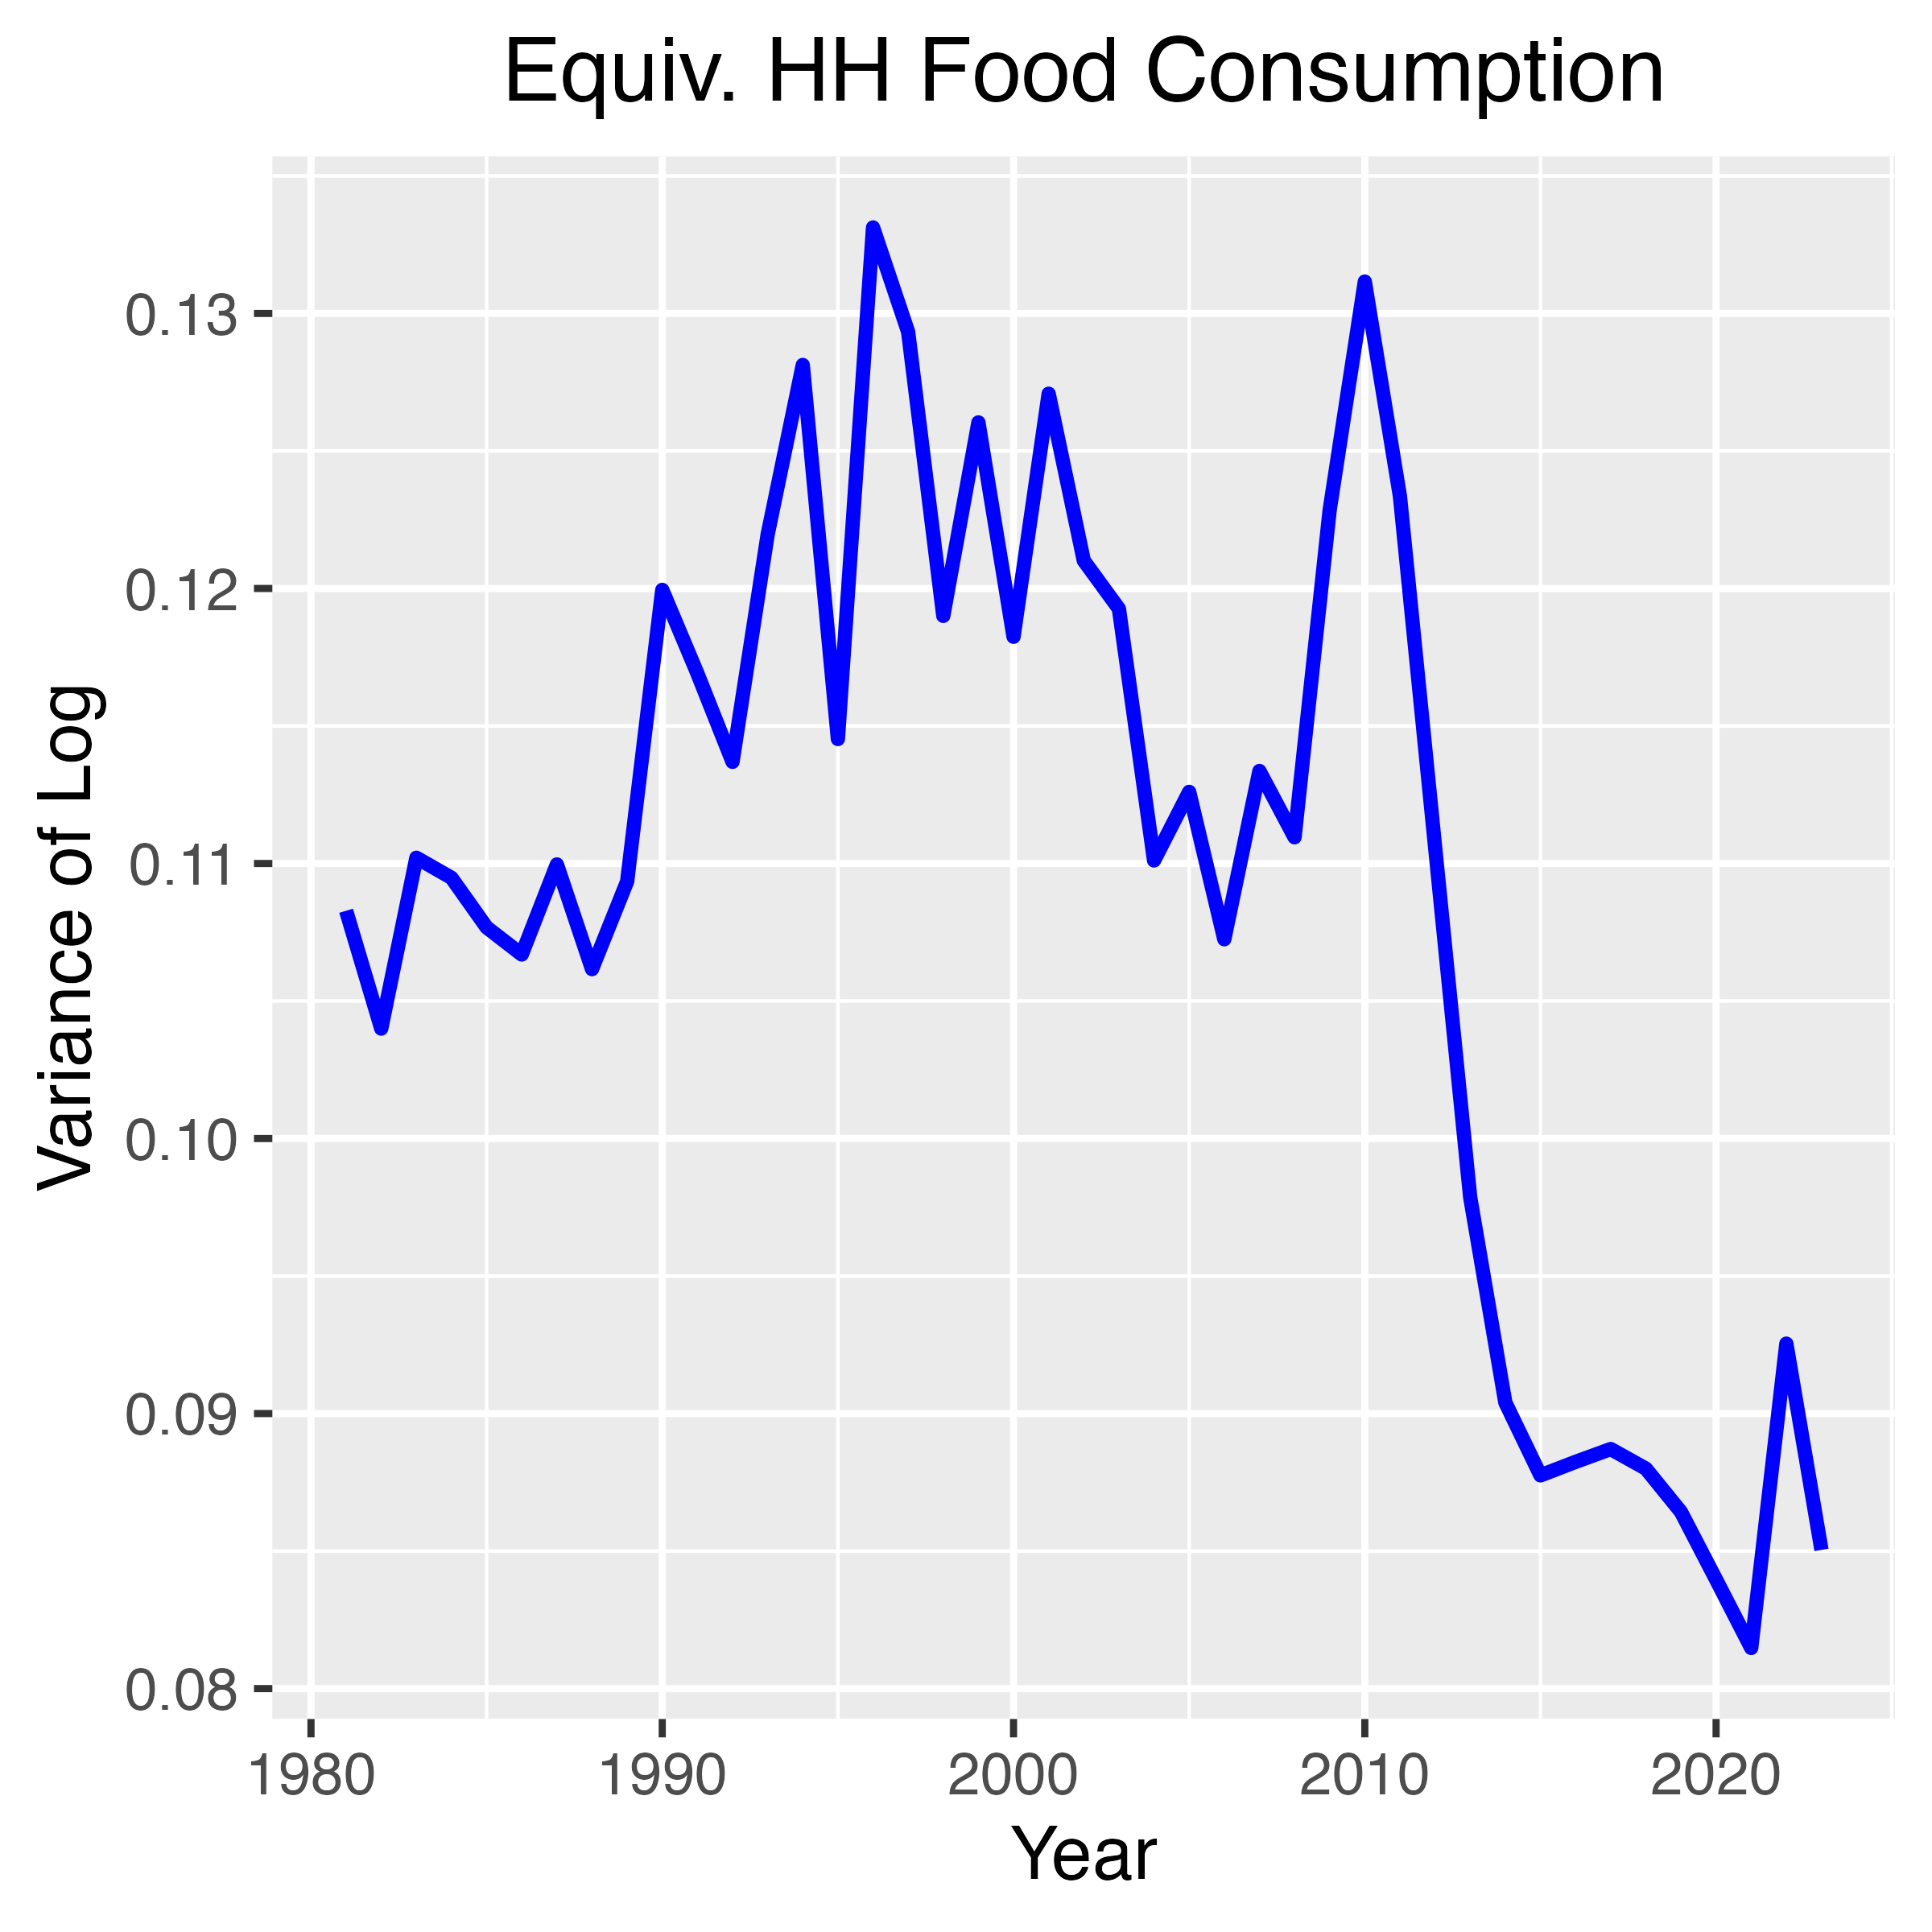
\includegraphics[width=\textwidth]{figures/Fig_8/Fig_8a_Var_Food.png}
    \end{subfigure}
    \begin{subfigure}[t]{0.475\textwidth}
        \centering
        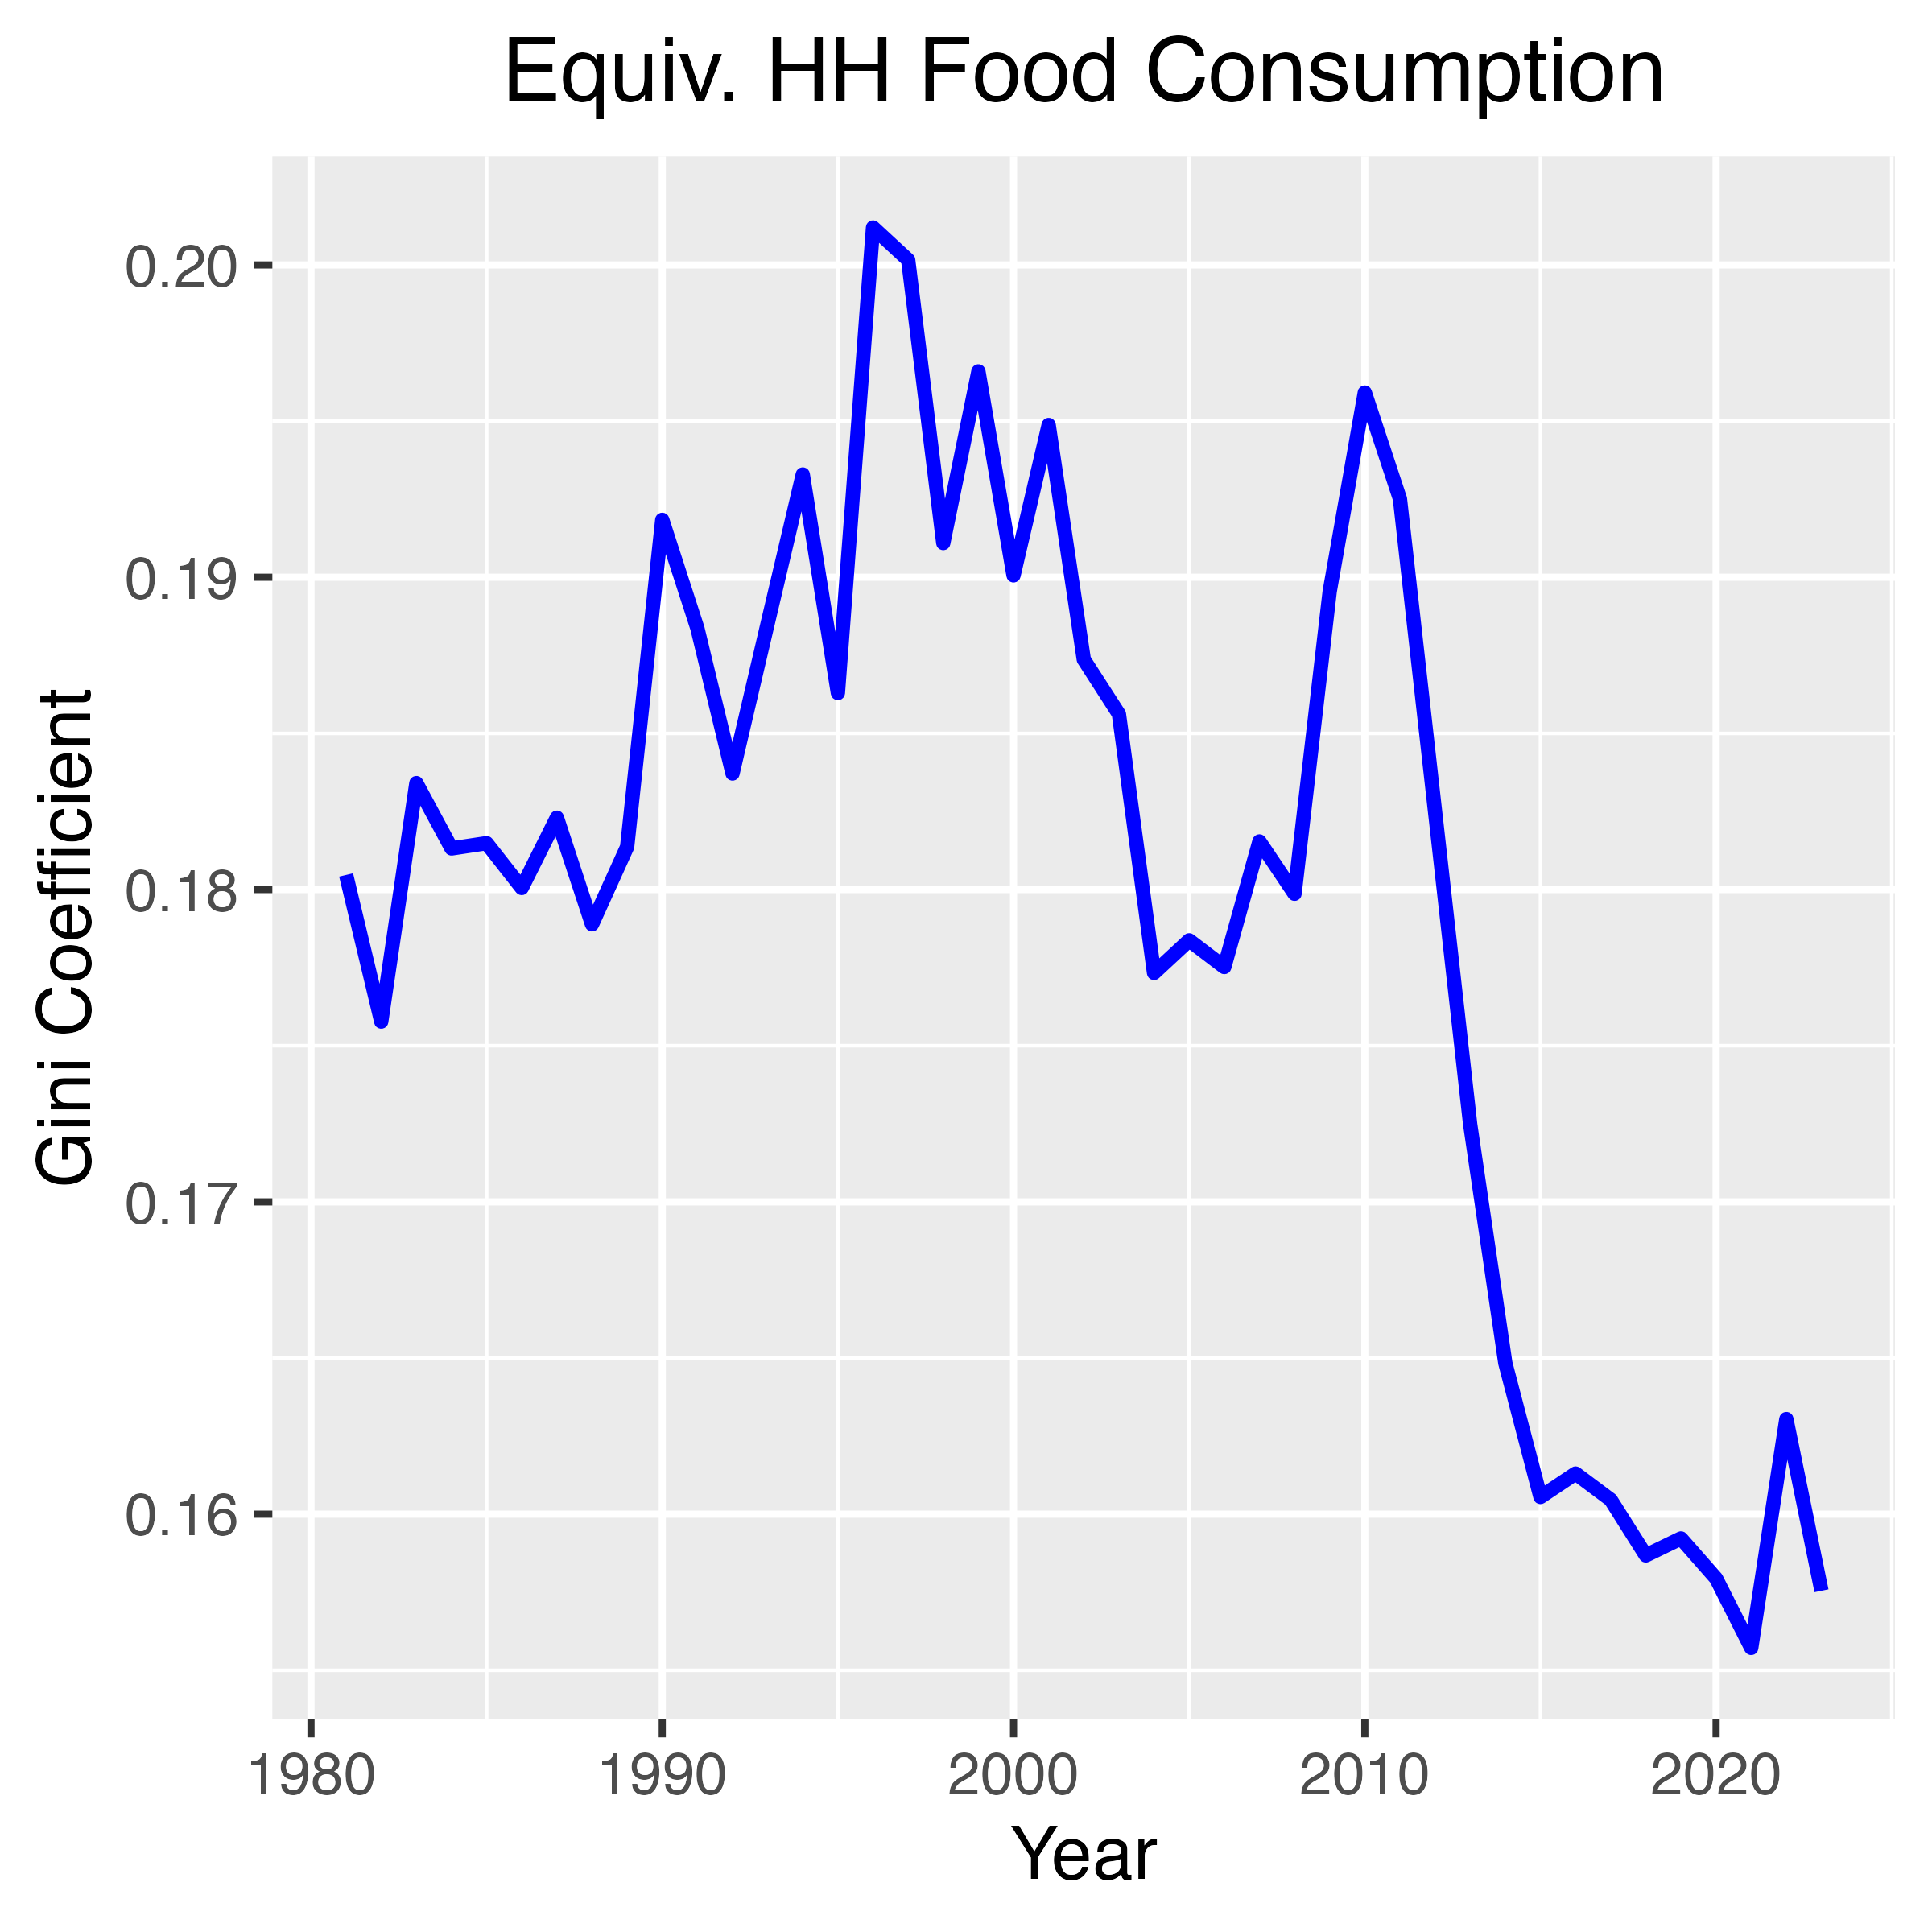
\includegraphics[width=\textwidth]{figures/Fig_8/Fig_8b_Gini_Food.png}
    \end{subfigure}
    \begin{subfigure}[t]{0.475\textwidth}
        \centering
        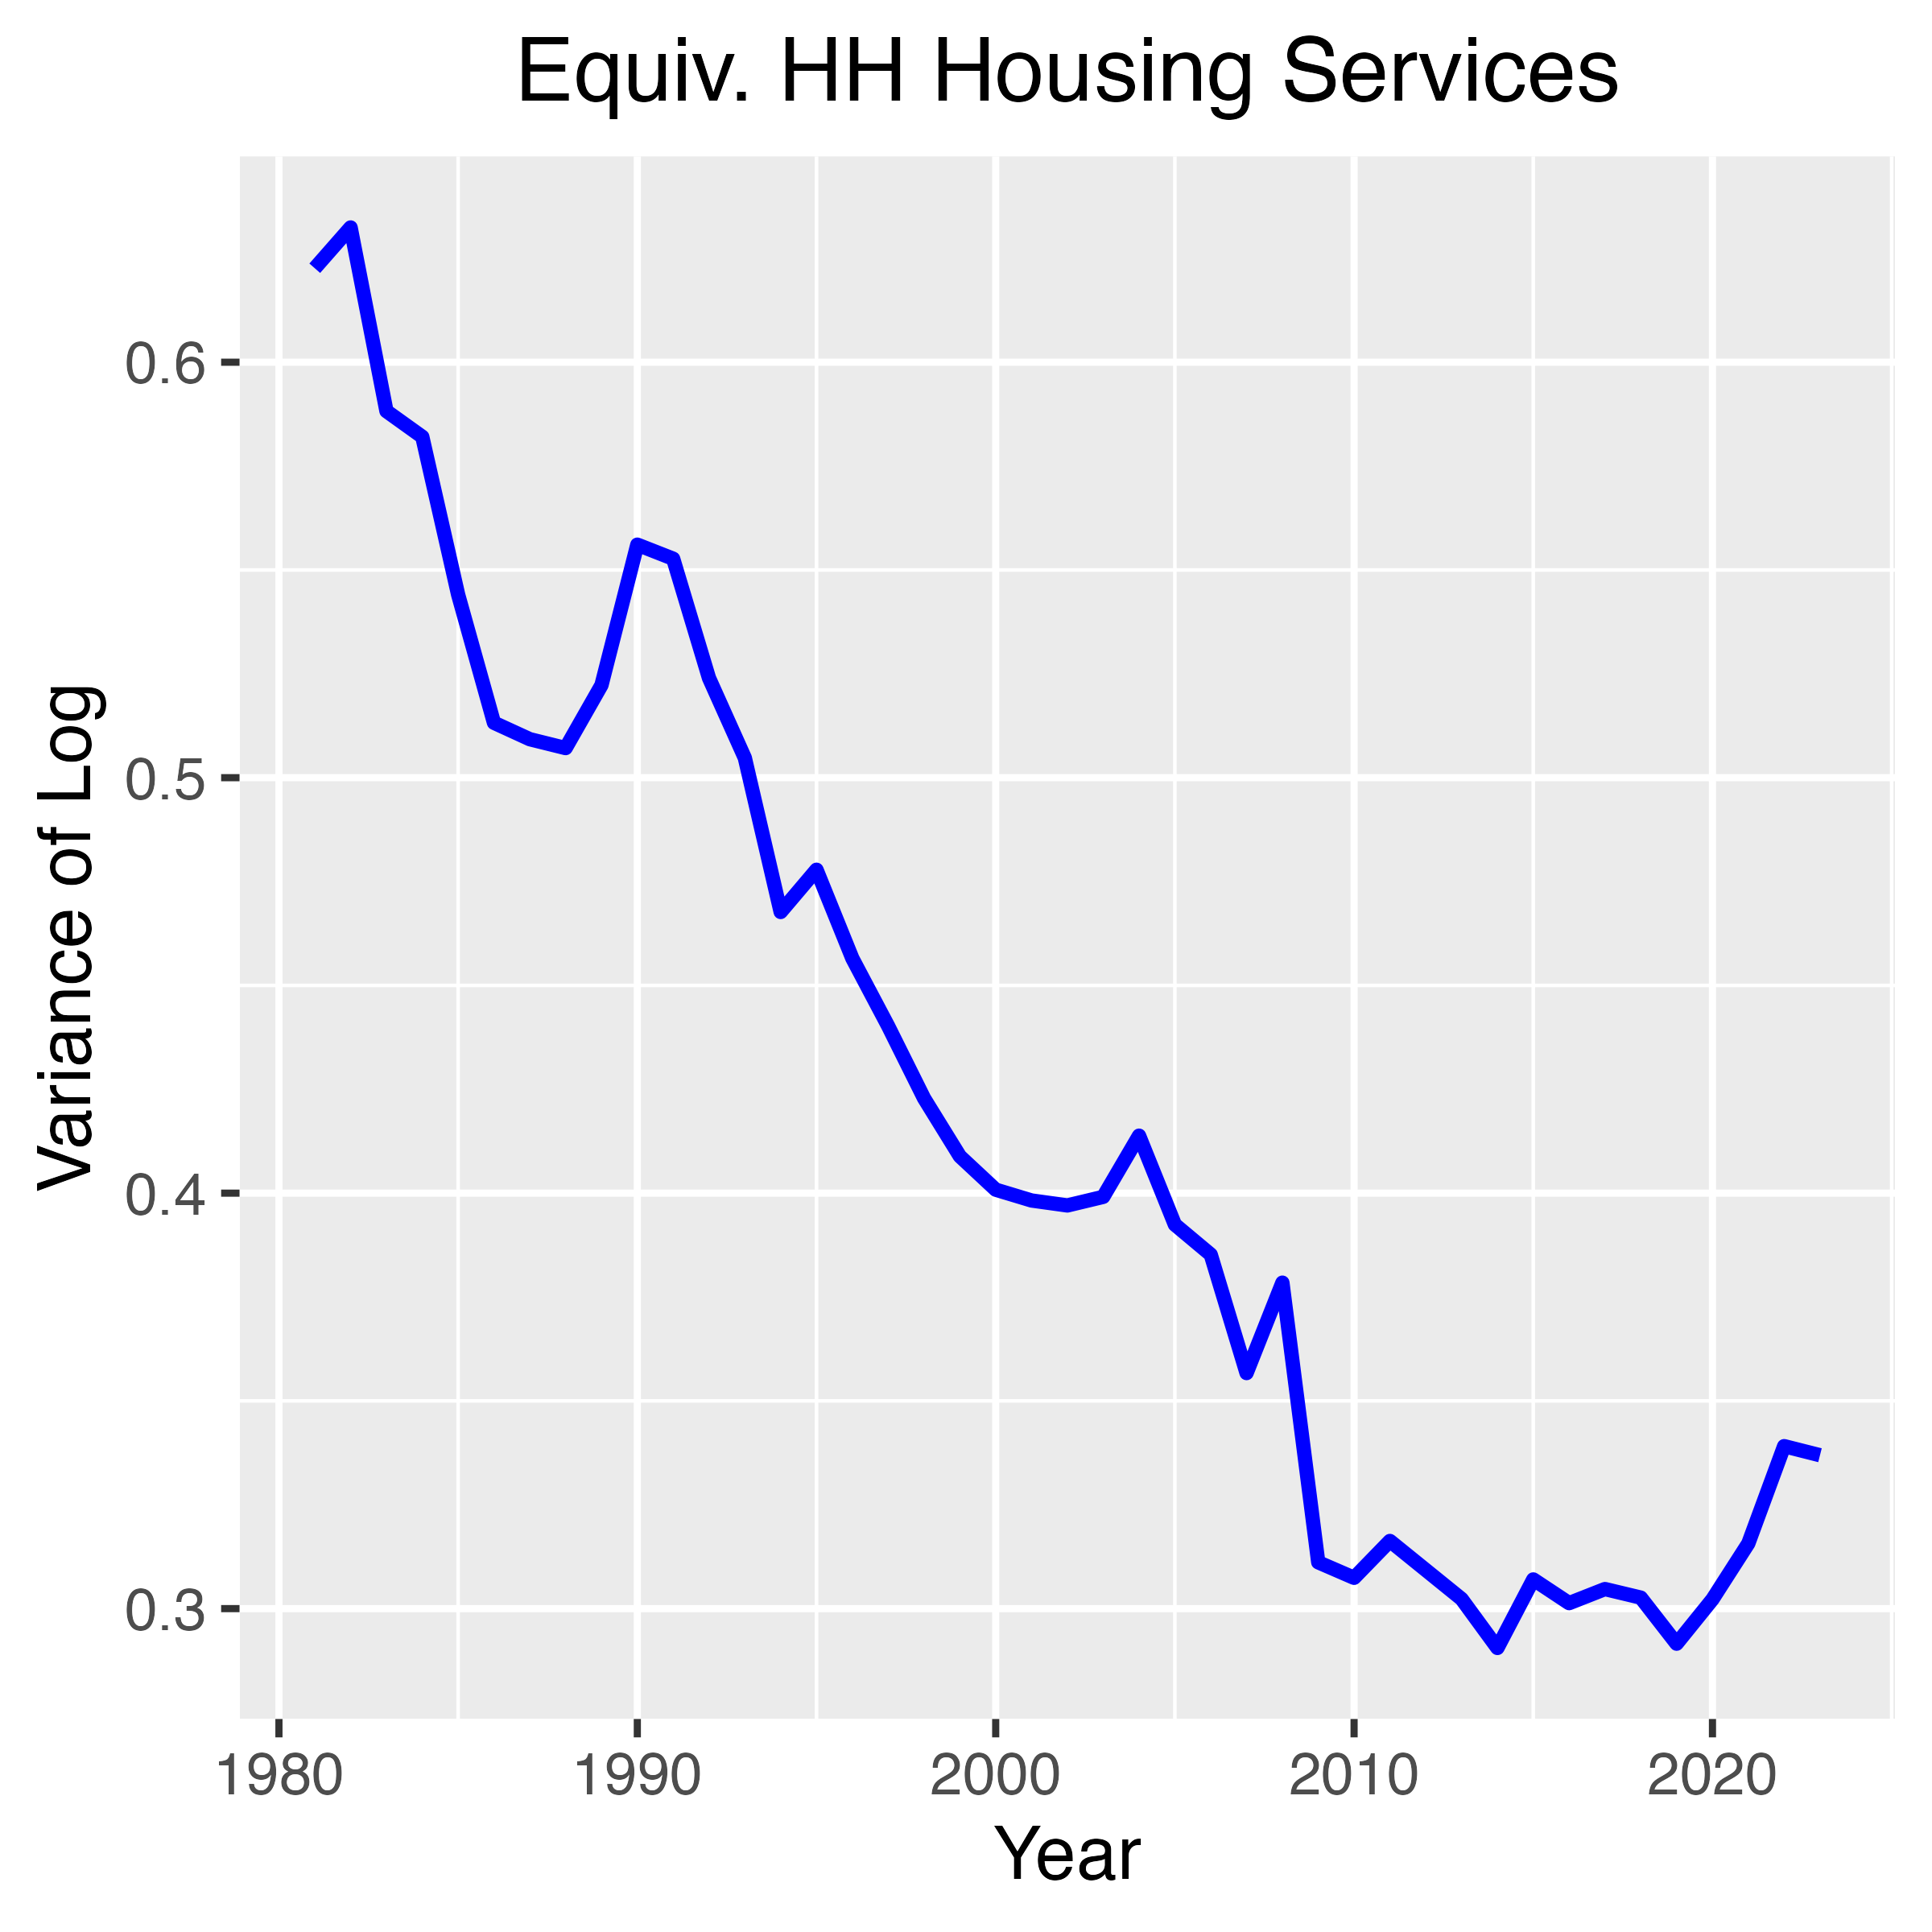
\includegraphics[width=\textwidth]{figures/Fig_8/Fig_8c_Var_Housing.png}
    \end{subfigure}
    \begin{subfigure}[t]{0.475\textwidth}
        \centering
        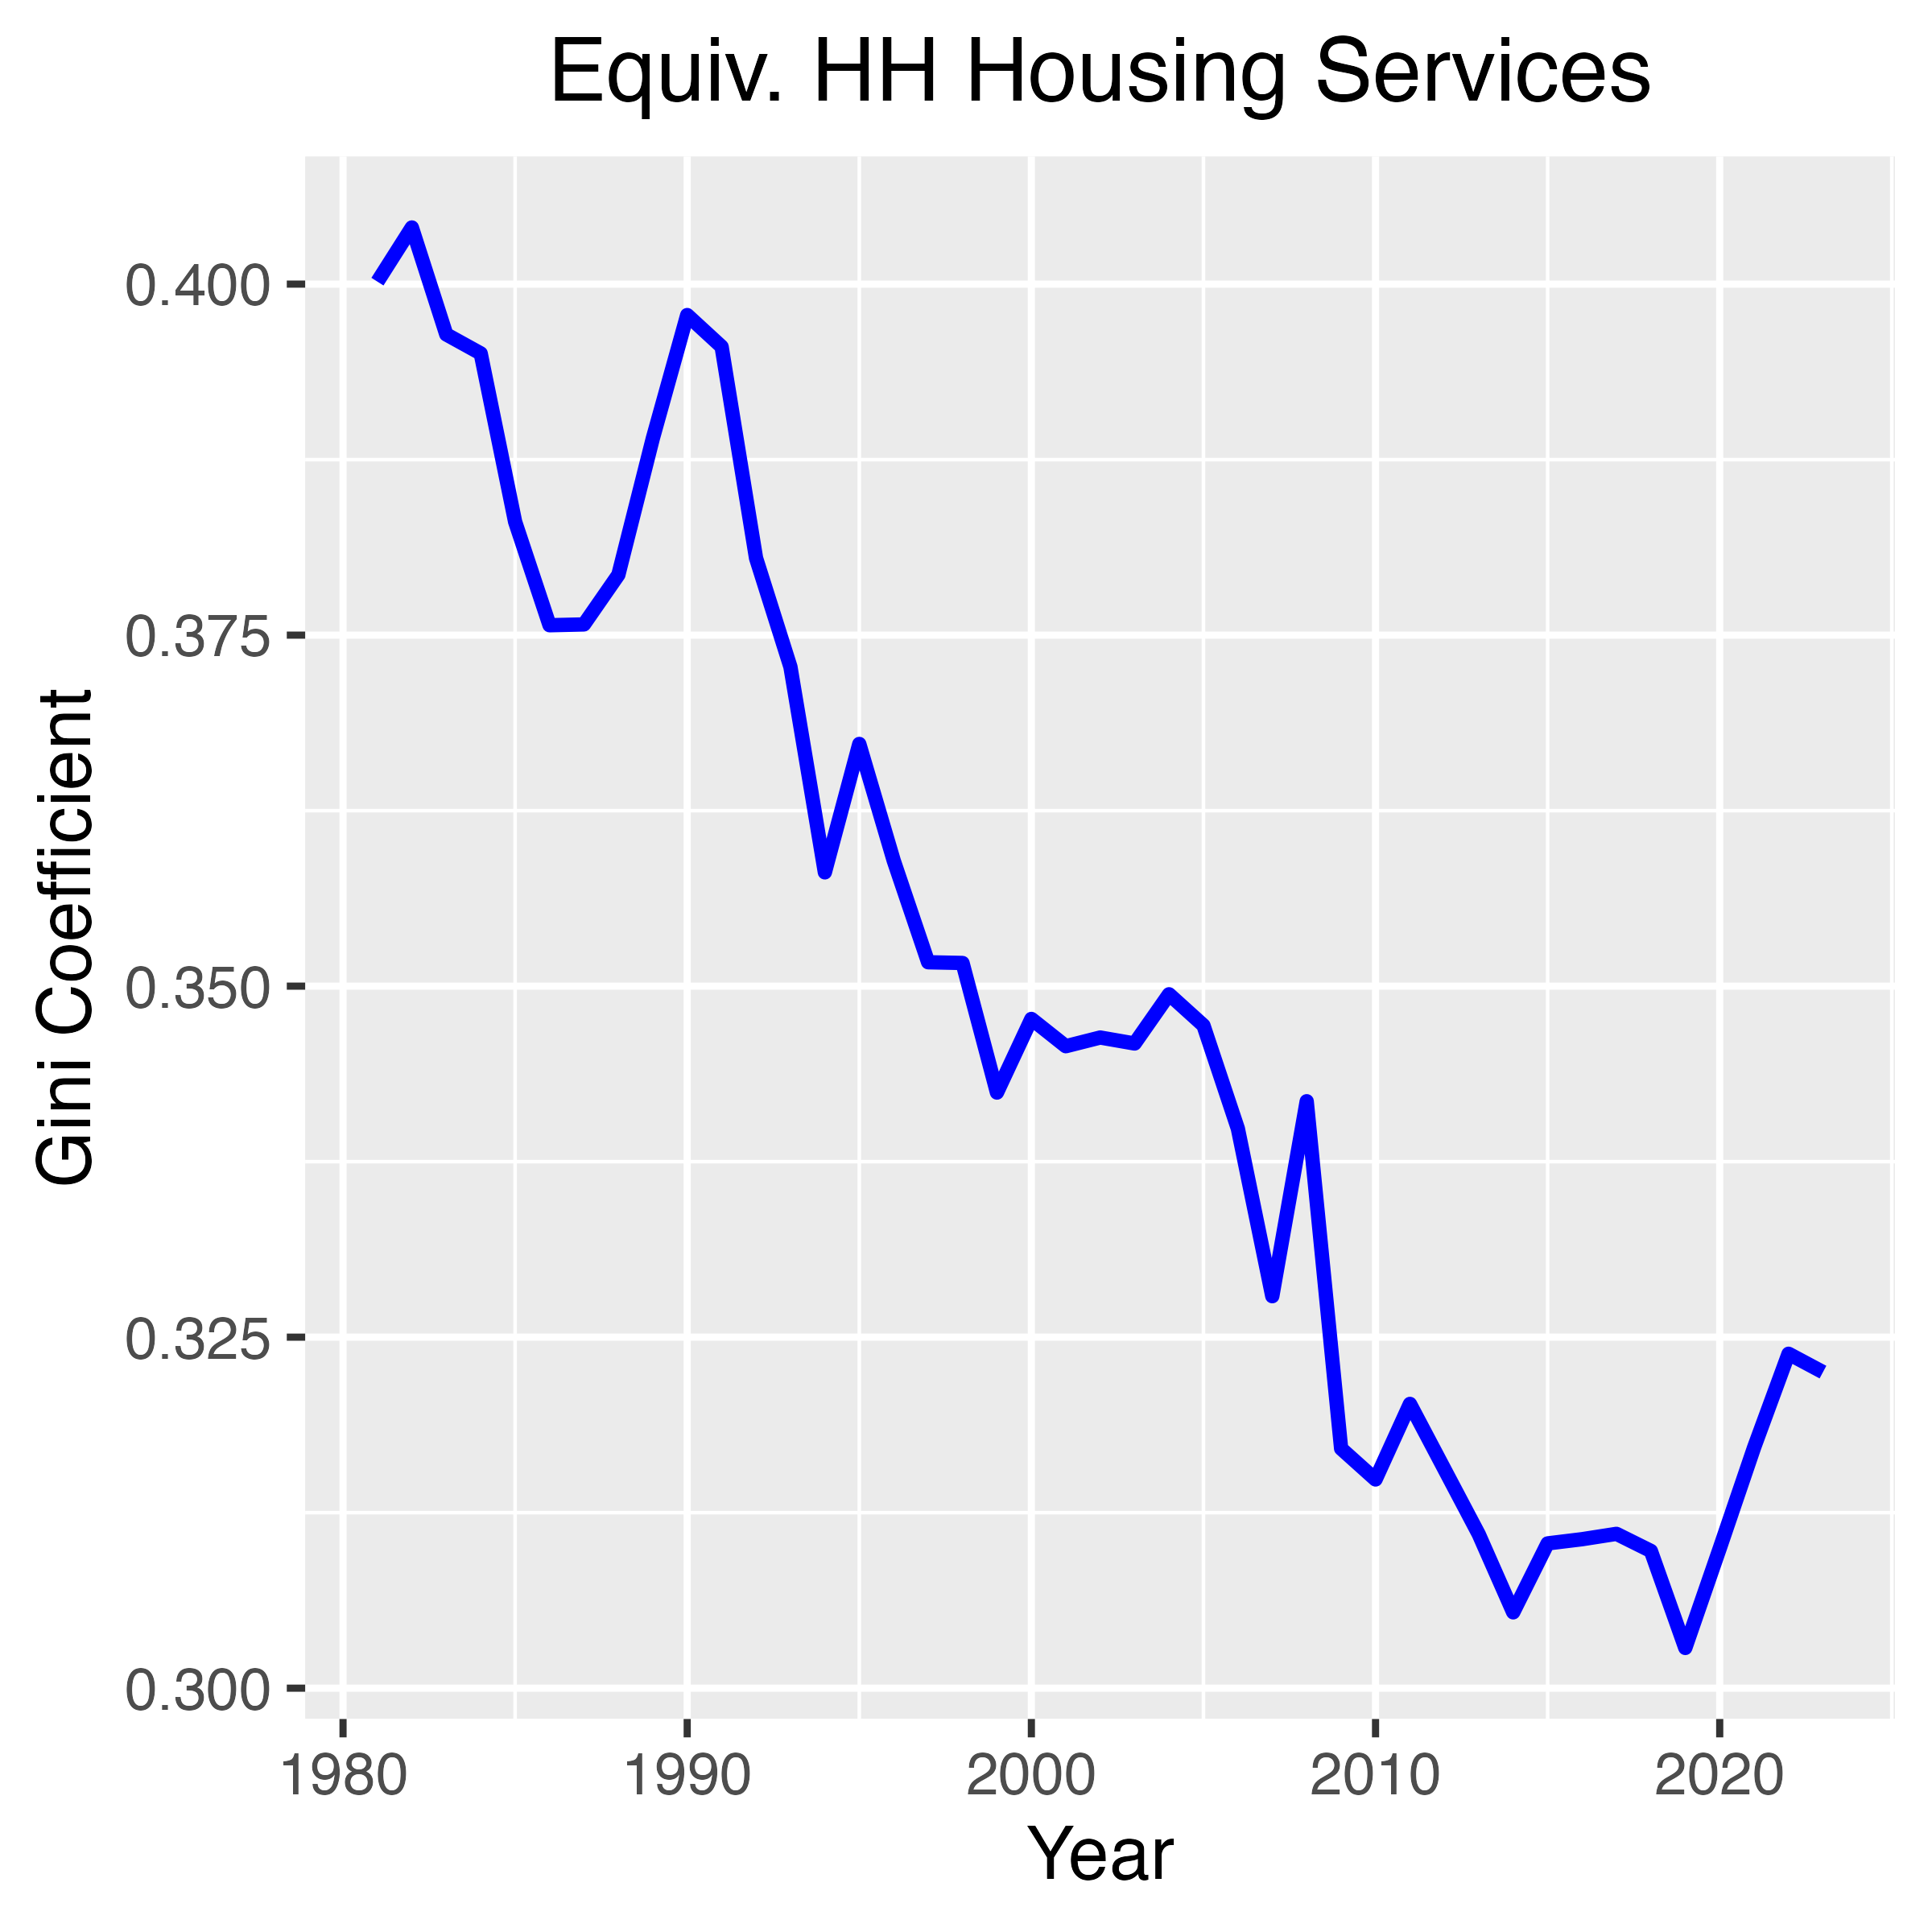
\includegraphics[width=\textwidth]{figures/Fig_8/Fig_8d_Gini_Housing.png}
    \end{subfigure}
    \caption{Food and Housing Consumption Inequality}
    \label{fig:Food_Housing}
\end{figure}

The final Figure \ref{fig:Food_Housing} highlights the inequalities in food and housing consumption in Taiwan. The Gini coefficients and variances presented in the figure indicate that the food expenditure discrepancies remain relatively small, and housing consumption inequality is steadily decreasing.

I do not have a strong theory about the decrease in food consumption inequality after 2010, maybe this is due to some change in the calculation of the SFIE.


\section{Conclusion}
\label{sec:conclusion}

This paper provides a comprehensive overview of the long-run evolution of income and consumption inequality in Taiwan from 1981 to 2023 using household-level data from the SFIE. The findings highlight several key trends and shifts over the past four decades. While income inequality has generally increased—especially since the mid-1990s—consumption inequality has remained relatively stable or declined, indicating the importance of consumption smoothing mechanisms such as saving, borrowing, and intra-family transfers.

The analysis shows that although the variance and Gini coefficient of household earnings have risen, the extent of inequality growth in Taiwan remains modest compared to advanced economies like the United States. Notably, inequality is most pronounced at the bottom of the earnings distribution, where low-income households have experienced stagnation or even decline, particularly during recessionary periods such as the Dot-com bubble, the Global Financial Crisis, and the COVID-19 pandemic.

Government redistribution through welfare programs and taxation has helped stabilize disposable income inequality, though its effectiveness varies across time and crises. The role of private transfers—especially since 2010—has also become more significant in mitigating inequality, emphasizing the extended family's role as a buffer.

Perhaps most intriguingly, the paper documents a declining trend in consumption inequality, driven partly by the low consumption growth of wealthy households and potentially concerning stagnation among higher-income groups. This divergence between income and consumption dynamics underscores the complexity of economic inequality and calls for more nuanced policy responses.

While Taiwan's inequality remains moderate by international standards, emerging structural shifts in family composition, consumption behavior, and income distribution point to growing vulnerabilities. Further work should investigate the causes behind these demographic, institutional changes and evaluate policies that could promote inclusive growth in an era of slower economic expansion.



% Format for bibliography
\DeclareFieldFormat[misc]{title}{{#1}}
% Format for citations
\DeclareFieldFormat[misc]{citetitle}{{#1}}  

\printbibliography

\newpage
% Appendices
\begin{appendices}
\section{Extra Figure for Cyclical Dynamics}
\label{sec:appendix_cyclical_dynamics}

\vspace{2em}

\begin{figure}[ht]
    \centering
    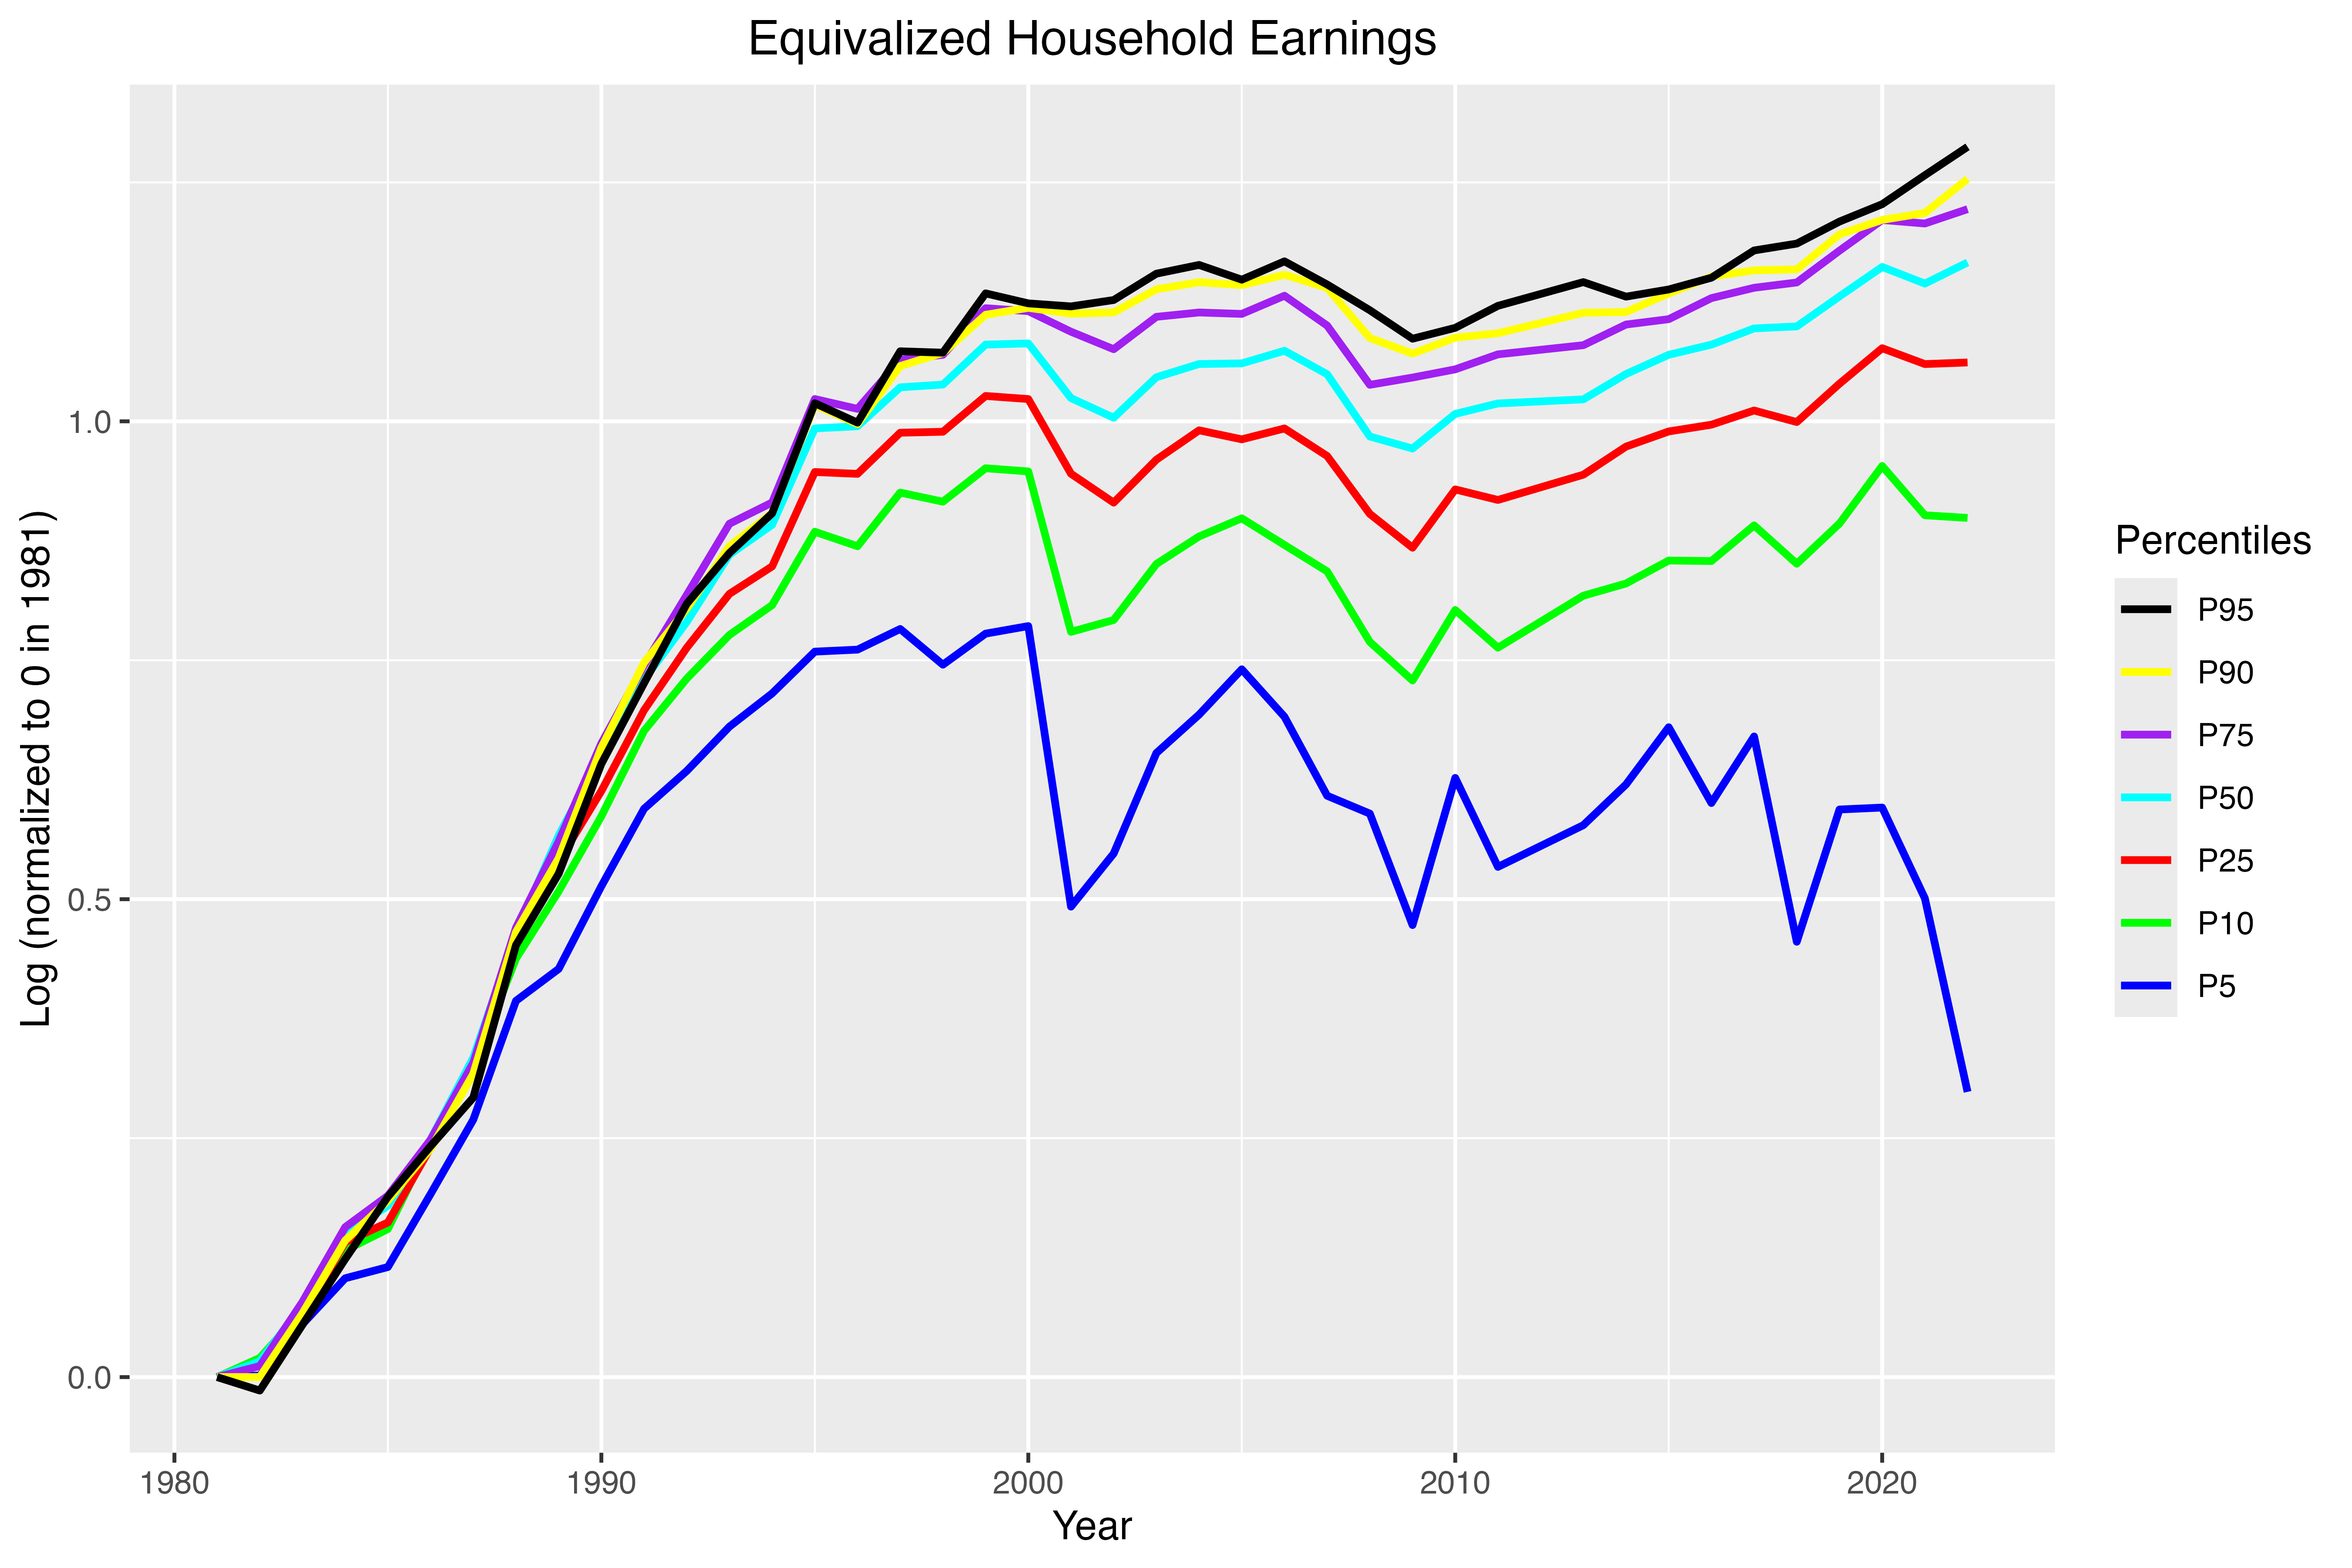
\includegraphics[width=0.88\textwidth]{figures/Fig_2/Fig_2_percentiles_1981.png}
    \caption{Percentiles of the Household Earnings Distribution, 1981 - 2023}
    \label{fig:appendix_cyclic_earnings_1981}
\end{figure}

\vspace{4em} 

\begin{figure}[ht]
    \centering
    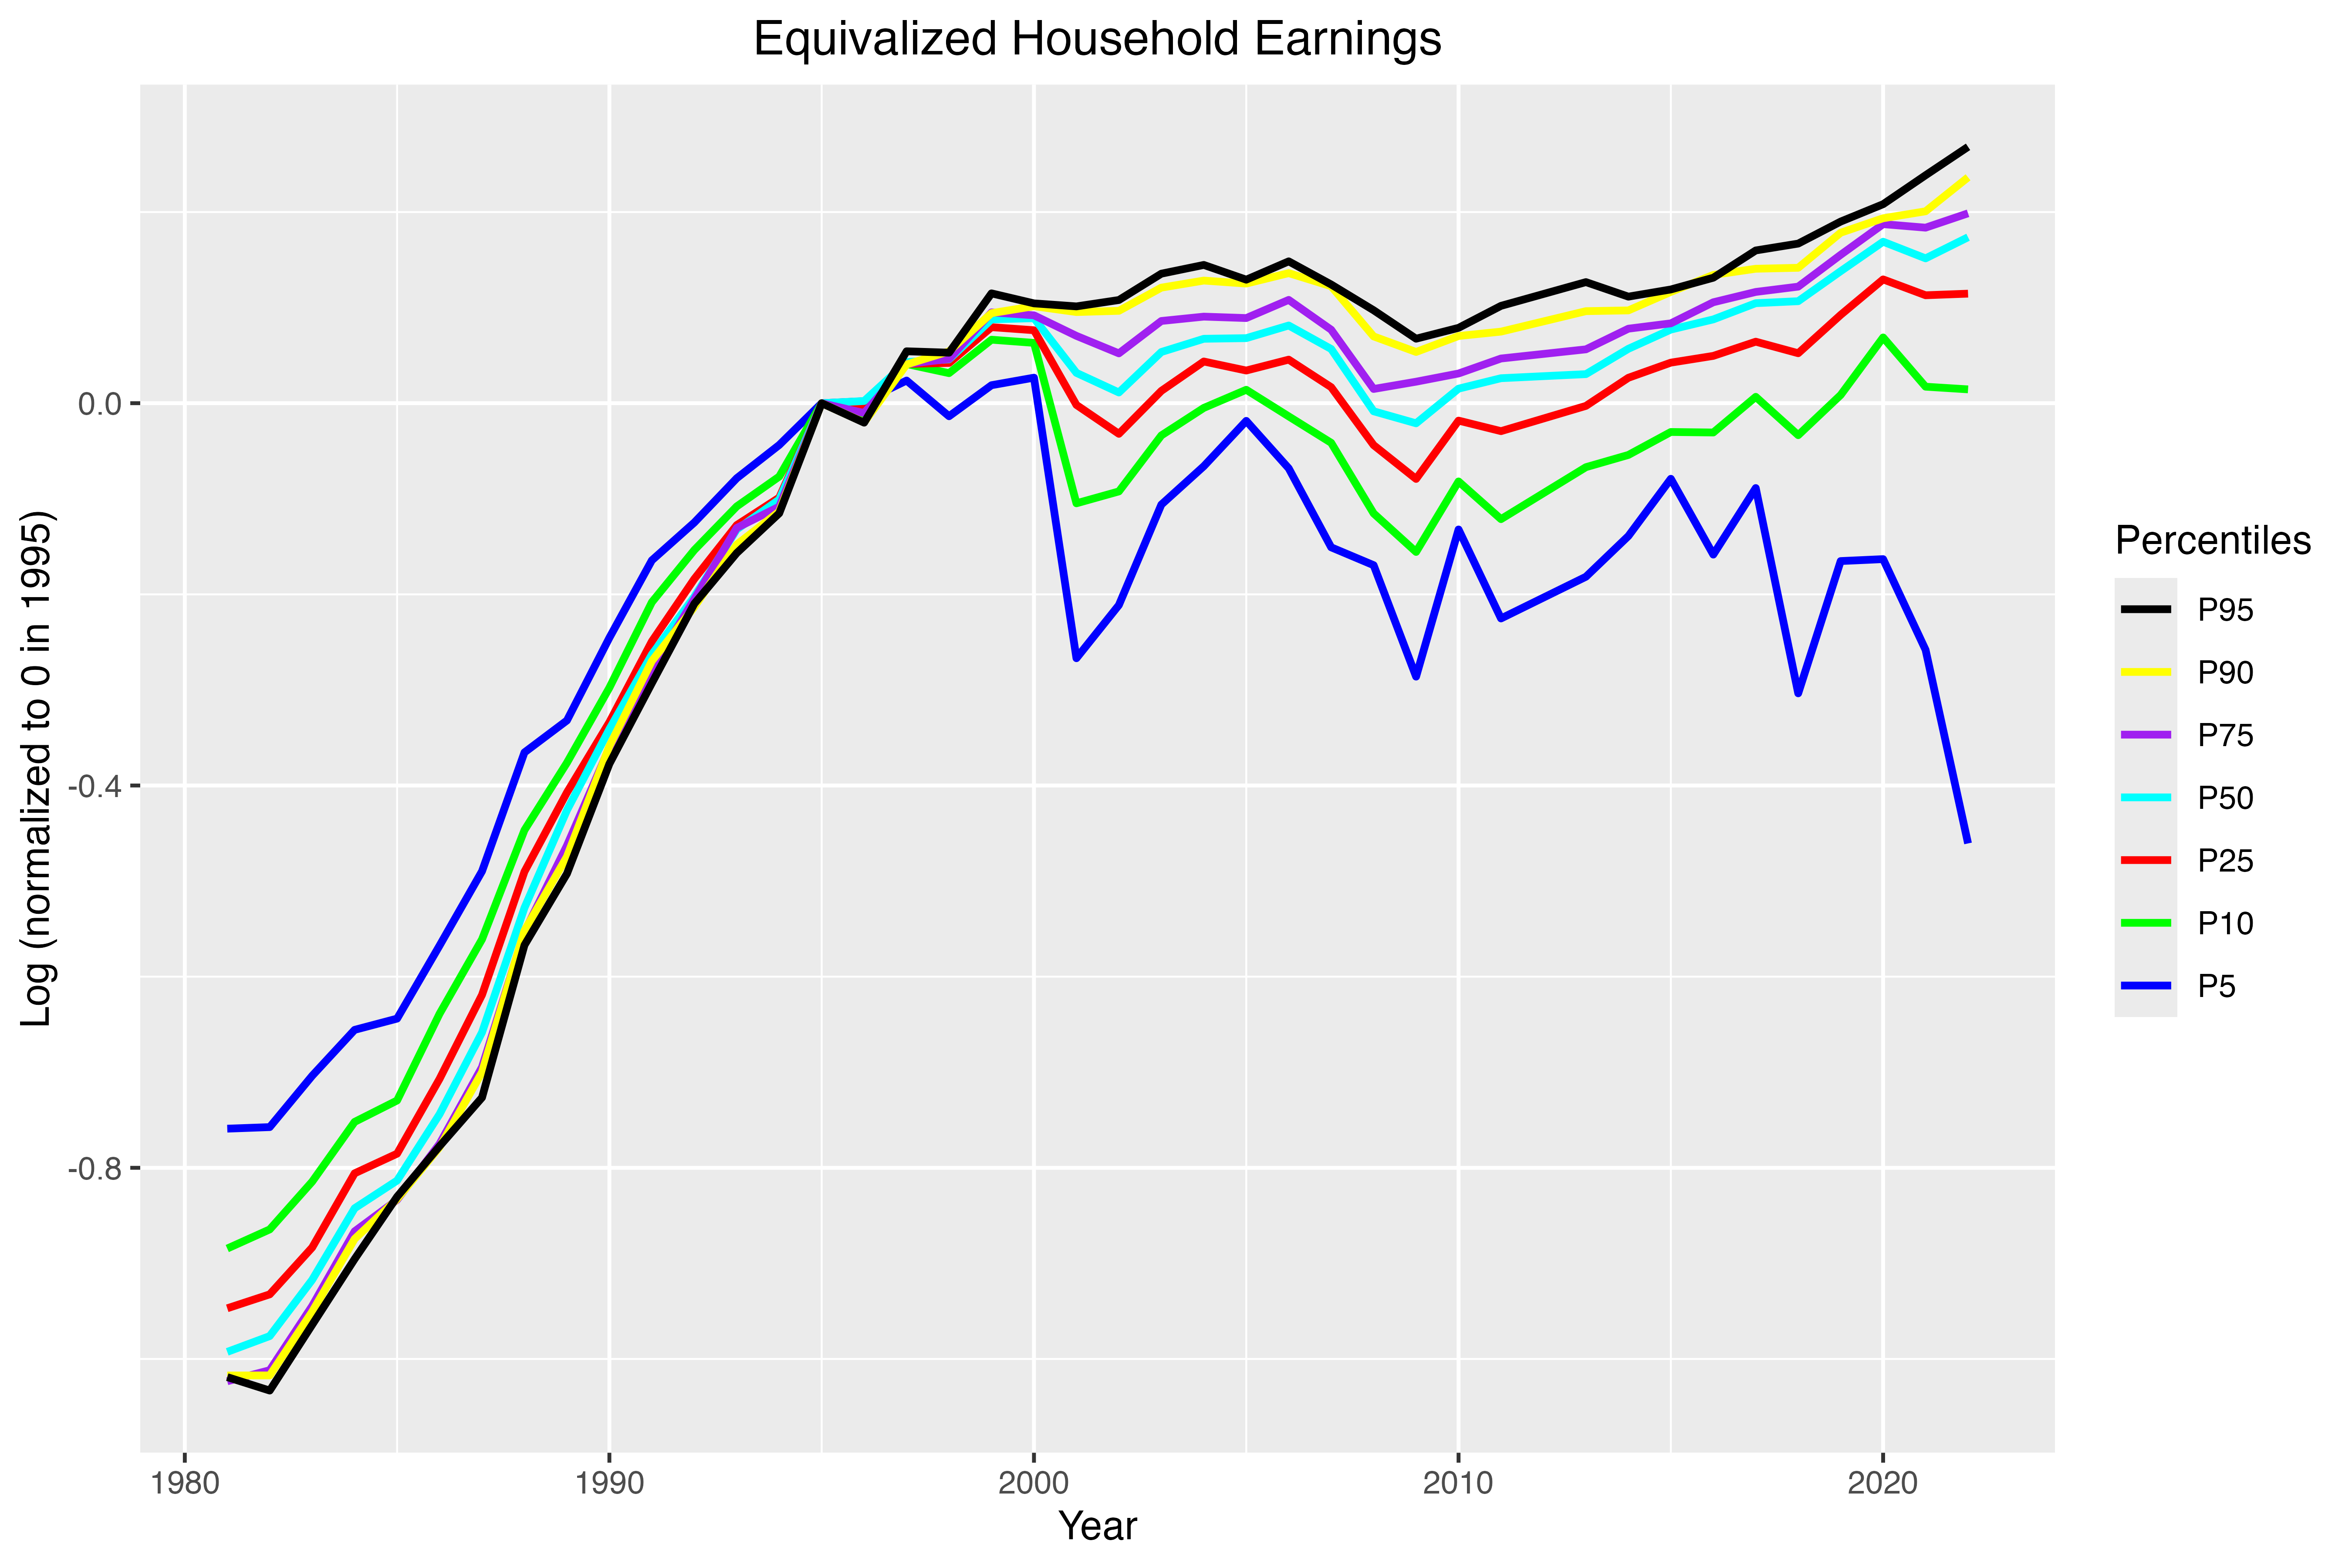
\includegraphics[width=0.88\textwidth]{figures/Fig_2/Fig_2_percentiles_1995.png}
    \caption{Percentiles of the Household Earnings Distribution, 1981 - 2023}
    \label{fig:appendix_cyclic_earnings_1995}
\end{figure}

\begin{figure}[ht]
    \centering
    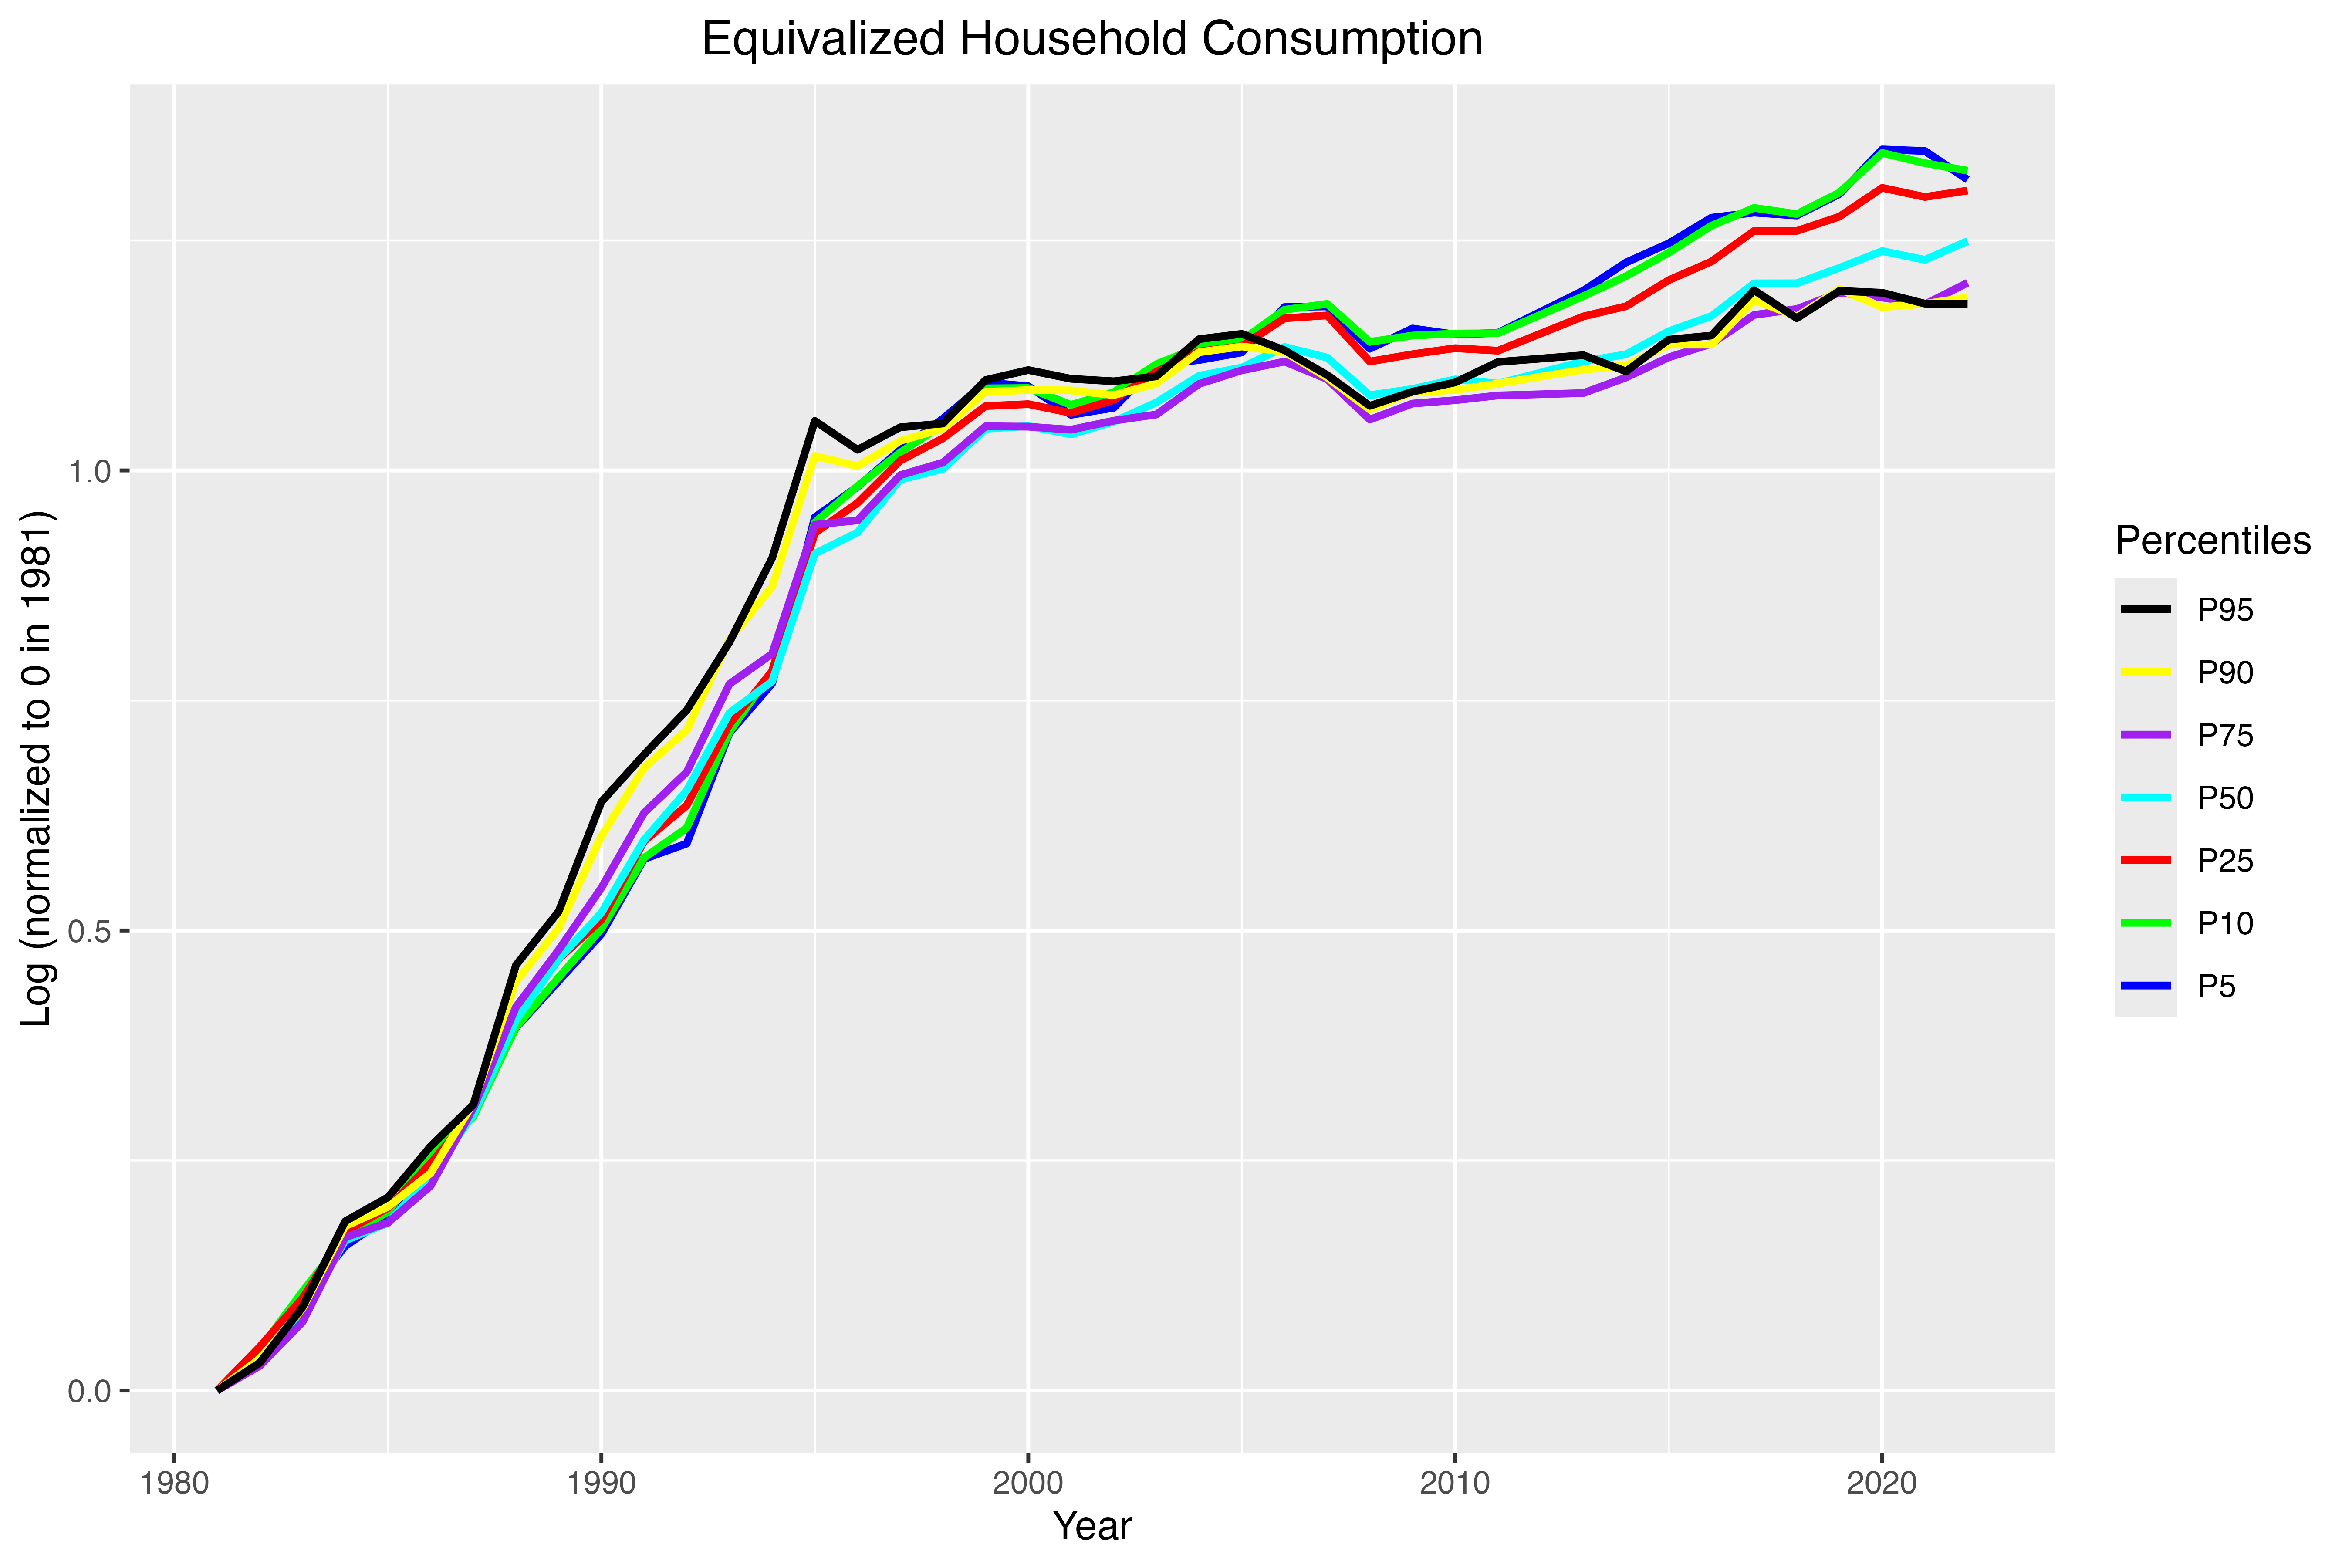
\includegraphics[width=0.88\textwidth]{figures/Fig_7/Fig_7_percentiles_1981.png}
    \caption{Percentiles of the Household Consumption Distribution, 1981 - 2023}
    \label{fig:appendix_cyclic_consumption_1981}
\end{figure}

\begin{figure}[ht]
    \centering
    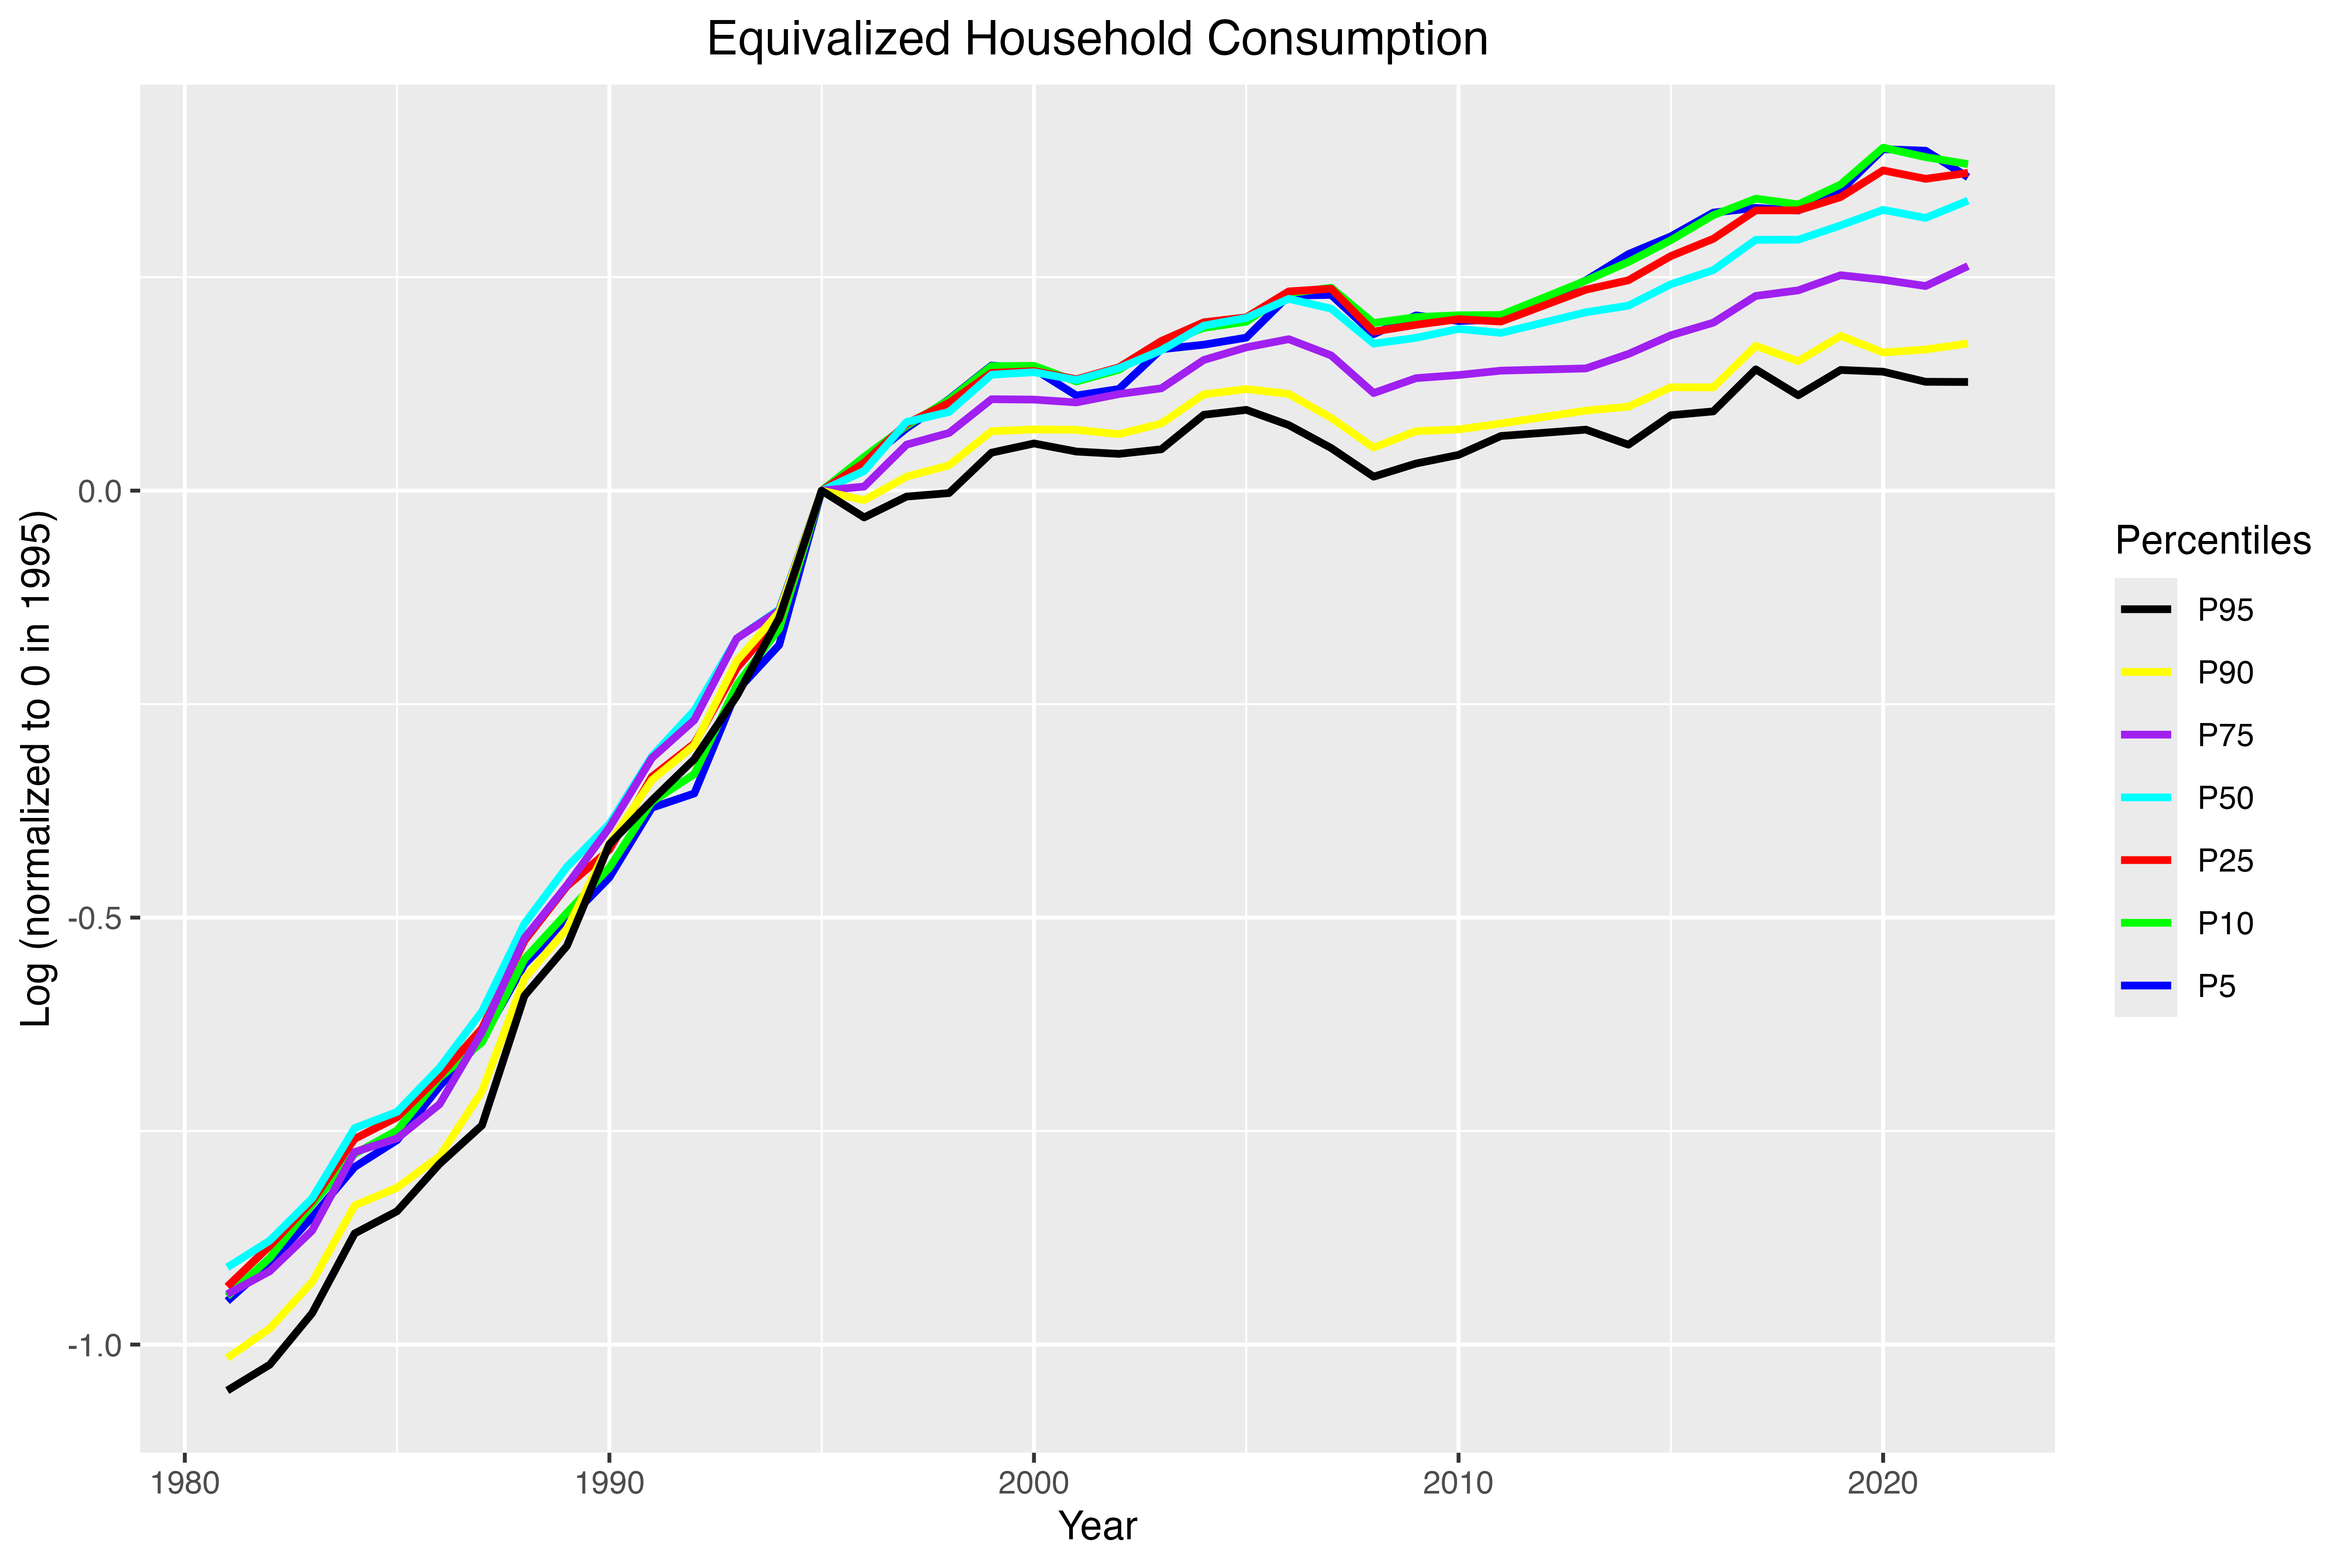
\includegraphics[width=0.88\textwidth]{figures/Fig_7/Fig_7_percentiles_1995.png}
    \caption{Percentiles of the Household Consumption Distribution, 1981 - 2023}
    \label{fig:appendix_cyclic_consumption_1995}
\end{figure}

\end{appendices}

\end{document}